% NAACL 2026 submission draft. Built on the ACL style files (acl.sty, acl_natbib.bst).
% Change "review" to "final" for the camera-ready version.
\documentclass[11pt]{article}
\usepackage[review]{acl}
\usepackage{times}
\usepackage{latexsym}
\usepackage[T1]{fontenc}
\usepackage[utf8]{inputenc}
\usepackage{microtype}
\usepackage{url}
\usepackage{inconsolata}
\usepackage{graphicx}
\usepackage{booktabs}
\usepackage{amsmath,amssymb}
\usepackage{multirow}
\usepackage{xcolor}
\usepackage{tikz}
\usetikzlibrary{arrows.meta,positioning,calc}
% entity colors shared with the data figures (Okabe-Ito): ours, baseline, per-layer routers
\definecolor{cDag}{HTML}{D55E00}
\definecolor{cDense}{HTML}{6E6E6E}
\definecolor{cLocal}{HTML}{009E73}

\newcommand{\dagf}{DAGFormer}
\newcommand{\dense}{dense OLMo-2}
\newcommand{\todo}[1]{\textcolor{red}{[#1]}}
\newcommand{\valpha}{\boldsymbol{\alpha}}
\newcommand{\pend}{\textcolor{black!45}{\textit{run.}}}

\title{One Predictor, One Graph: Learning a Transformer's\\Cross-Layer Topology from Its Tokens}
%alternative title: small topology predictors learn to route dynamic attention of large language models across layers and heads

\author{Anonymous NAACL submission}

\begin{document}
\maketitle

\begin{abstract}
A layer in a Transformer model transmit information to deeper layers through a shared residual stream during the forward pass. Recent architectures improve on this standard design with per-token routing: every layer reads all earlier layers' outputs through weights that depend on the input. They share one defect: each layer chooses its inputs with a router of its own, so no module takes a global view of the routing structure throughout the model. In this work, we propose \dagf{}, in which a small predictor, jointly pretrained with the Transformer, reads only the input tokens and plans the cross-layer graph of the whole model before the backbone runs. On matched OLMo-2 pairs from 75M to 1B parameters, \dagf{} lowers held-out loss at every size and at equal compute with the routing cost charged, by a margin that grows with size; a 1B \dagf{} trained on half the tokens beats the dense 1B model, and the gain is consistent across benchmarks and carries to evaluations after instruction tuning. The learned graph also makes models degrade more gracefully under structured pruning, without any re-routing.
\end{abstract}

\section{Introduction}

A Transformer \citep{vaswani2017} composes its layers through residual connections \citep{he2016resnet}: every attention head and MLP reads the same running sum and writes back into it. Mechanistic analyses describe this residual stream as the communication channel between components \citep{elhage2021}. Its width is shared by every layer, so which earlier computation a layer can read is fixed by design: a late layer sees an early result only inside a sum to which every intermediate layer has added its own.

A line of work relaxes this fixed connectivity. Dense connections \citep{huang2017densenet} and depth-weighted averaging with learned static weights \citep{pagliardini2024denseformer} let a layer read earlier layers' outputs directly. Hyper-connections \citep{zhu2024hyperconnections} widen the residual stream into several streams whose mixing weights are learned and, in the dynamic variant, input-dependent, and mHC \citep{mhc2026} constrains those mixing matrices so the scheme trains stably at scale. Multiway dynamic dense connections \citep{muddformer2025} compute input-dependent weights over all earlier layers' outputs, separately for the query, key, value and residual inputs of a block. These models reach the loss of Transformers trained with substantially more compute \citep{zhu2024hyperconnections,muddformer2025}.

All of the dynamic variants make the same design decision: routing is \emph{local}. Each layer carries its own router, which reads that layer's current hidden state and decides what that layer reads. The cross-layer graph is therefore assembled greedily, one layer at a time, and no component of the model holds it. Three things follow. The graph cannot be planned jointly from the input. It cannot be inspected, frozen or replaced as an object. And one cannot tell whether the gain comes from per-token re-routing or from the connections themselves, because removing a per-layer router removes its connections too.

We propose to predict the whole topology with one separate module that reads only the input, before the backbone runs. One module then serves every layer, so its parameters are shared across depth. The topology exists as an object before the first layer is computed, so it can be read, averaged over tokens, frozen or swapped between inputs. And the local design remains available as an optional second channel, which lets the two sources of routing be compared inside one model. A topology computed before the backbone runs also serves a broader aim. Post-hoc interpretability explains a computation only after it has produced its output, whereas generative interpretability asks that a model's inference pass expose checkpoints that humans can understand and that can be causally intervened on before the output is committed \citep{yang2026generative}. A predicted topology meets the second requirement by construction, since the backbone depends on it and replacing it is a well-defined intervention; whether it can also be made understandable to humans is a question this design opens.

\dagf{} implements this design with a small causal encoder over the token ids (Figure~\ref{fig:arch}). For every layer and attention head it emits mixing weights over the embedding and all earlier layer outputs for the head's query, key and value inputs, and for every layer a mixing for its residual input. The backbone is an unchanged OLMo-2 \citep{olmo2} whose per-layer inputs are replaced by these mixtures. At initialization the weights select only the previous layer, so training starts from exactly the dense model; a variant adds zero-initialized per-layer routers on the hidden state, the local design of prior work.

We train matched pairs of dense OLMo-2 and \dagf{} from 75M to 1B parameters on Dolma \citep{soldaini2024dolma} and charge the routing cost in every compute comparison. \dagf{} is better at every size and at equal compute, by a margin that grows with size, and the gain survives instruction tuning and a judged chat comparison; dense models given the routing parameters as extra width close most of the gap at the smallest size and less than half of it at the next. Trained with the same pipeline, static cross-layer weights recover little of the gain, and a per-layer-router baseline is behind at two sizes and ahead at one. Ablations show that a shared predictor matches per-layer routers and beats unshared per-layer predictors with fewer parameters. Under structured pruning during finetuning, \dagf{} degrades more gracefully than dense models in all but one setting and than the per-layer-router baselines, and freezing its predictor changes nothing. 

\textbf{Our contributions are as follows:}
\begin{itemize}\setlength\itemsep{0pt}
\item \dagf{}, a Transformer whose per-head cross-layer topology is emitted by one separate predictor over the tokens, trained jointly from the dense model (Section~\ref{sec:method}).
\item A matched scaling study from 75M to 1B with the routing cost charged and with DenseFormer, hyper-connection, mHC and MUDDFormer baselines on the same pipeline, carried through instruction tuning and judged chat (Section~\ref{sec:experiments}).
\item Ablations of the routing source and a structured-pruning study showing that the learned graph makes models degrade more gracefully, without re-planning by the predictor (Sections~\ref{sec:analysis}, \ref{sec:pruning} and~\ref{sec:discussion}).
\end{itemize}

\begin{figure*}[t]
\centering
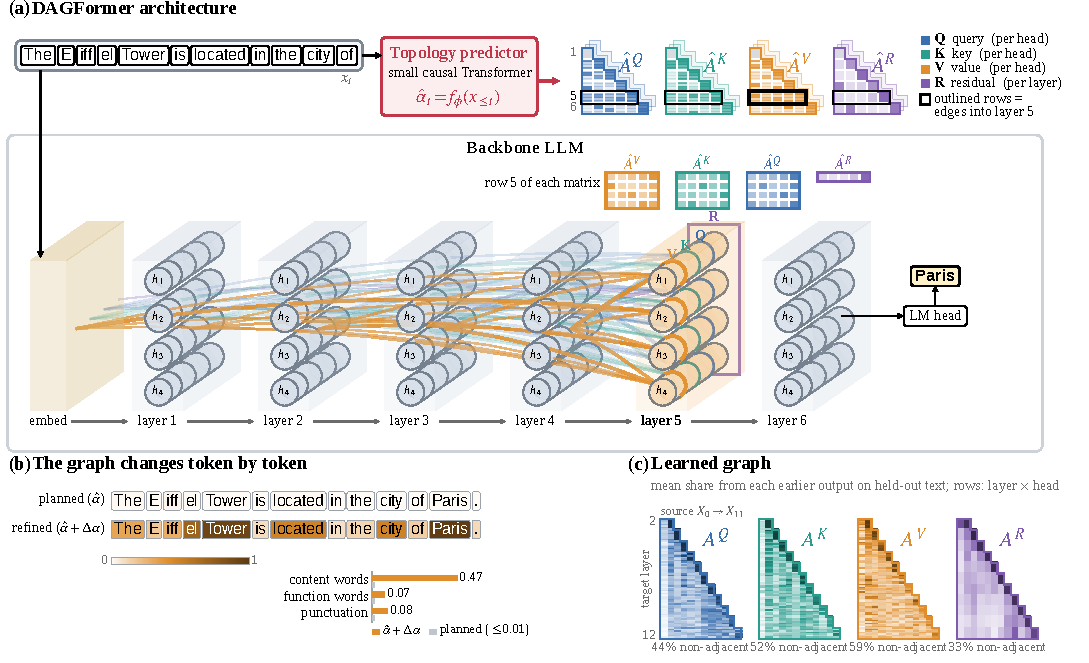
\includegraphics[width=\textwidth]{figures/fig1_architecture.pdf}
% \resizebox{0.86\textwidth}{!}{% figures/method.tex -- Figure 1: the DAGFormer method, drawn in TikZ (vector; no raster).
% Used from main.tex as   \resizebox{0.86\textwidth}{!}{% figures/method.tex -- Figure 1: the DAGFormer method, drawn in TikZ (vector; no raster).
% Used from main.tex as   \resizebox{0.86\textwidth}{!}{% figures/method.tex -- Figure 1: the DAGFormer method, drawn in TikZ (vector; no raster).
% Used from main.tex as   \resizebox{0.86\textwidth}{!}{\input{figures/method}}
% Needs: tikz (arrows.meta, calc), xcolor; \valpha (bold alpha) from main.tex.
%
% Layout (top-down data flow): the token row at the top feeds the topology predictor (top left) and the
% backbone embedding X_0 (right). The predictor is a horizontal pipeline ending in four colored outputs
% (q, k, v, R); the lower-left panel shows the weights a trained model learned, averaged over tokens. In the backbone (right),
% each layer's mixer (four colored strips: q, k, v, R) reads every earlier output X_j through colored
% curves that loop through the corridor left of the layer bands; the band output is X_l.
\providecommand{\valpha}{\boldsymbol{\alpha}}
\definecolor{cQ}{HTML}{0072B2}
\definecolor{cK}{HTML}{E69F00}
\definecolor{cV}{HTML}{009E73}
\definecolor{cR}{HTML}{CC79A7}
% The lower-left grids are the learned routing weights of DAGFormer-300M, generated from data by
% figures/gen_method_alpha.py into figures/method_alpha.tex (cells, outlines and frames).
\begin{tikzpicture}[x=1cm, y=1cm, font=\footnotesize, >=Stealth, line cap=round, line join=round,
  box/.style={draw=black!70, fill=white, rounded corners=1.5pt, inner sep=2pt, align=center},
  pbox/.style={box, fill=black!4, font=\scriptsize, minimum height=10.5mm},
  ob/.style={draw=none, rounded corners=1pt, minimum width=3mm, minimum height=2.4mm, inner sep=0pt, font=\tiny},
  src/.style={draw=black!70, fill=black!9, rounded corners=1.5pt, inner sep=1.5pt, minimum width=13mm, minimum height=4mm},
  band/.style={draw=black!70, fill=white, rounded corners=2pt, minimum width=39.5mm, minimum height=7.2mm, inner sep=0pt},
  head/.style={draw=black!60, fill=black!3, rounded corners=1pt, minimum width=4.2mm, minimum height=4mm, inner sep=0pt, font=\scriptsize},
  strip/.style={draw=none, inner sep=0pt, outer sep=0pt, minimum width=6mm, minimum height=1.8mm, font=\tiny},
  panel/.style={draw=black!50, rounded corners=3pt, line width=0.5pt, fill=black!2},
  ptitle/.style={font=\footnotesize\bfseries, inner sep=0pt},
  note/.style={font=\scriptsize, color=black!65, align=left, inner sep=1pt},
  flow/.style={->, black!75, line width=0.6pt},
  wire/.style={line width=0.45pt, opacity=0.85}]

% ---------------------------------------------------------------- panels
\draw[panel] (0.3,5.45) rectangle (8.05,8.1);
\draw[panel] (0.3,1.25) rectangle (8.05,5.15);
\draw[panel] (9.0,1.1) rectangle (16.3,8.1);
\node[ptitle, anchor=north east] at (7.9,7.98) {Topology predictor \normalfont(reads only the token ids)};
\node[ptitle, anchor=north west] at (0.45,5.03) {Learned routing weights $\valpha^{(l)}$ \normalfont(DAGFormer-300M)};
\node[ptitle, anchor=north east] at (16.15,7.98) {Backbone \normalfont(OLMo-2 decoder)};

% ---------------------------------------------------------------- input tokens (top)
\foreach \i/\t in {0/$x_1$,1/$x_2$,2/$x_3$,3/$\cdots$,4/$x_T$}
  \node[box, minimum width=7.5mm, minimum height=4.5mm, inner sep=1pt] (tok\i) at (10.35+0.85*\i, 8.75) {\t};
\node[note, anchor=east] at (9.85,8.75) {input tokens};

% ---------------------------------------------------------------- backbone sources + bands (right)
\node[src] (x0) at (12.05,7.42) {$X_0$ {\tiny(embedding)}};
\draw[flow] (12.05,8.5) -- (x0.north);
\fill[black!75] (12.05,8.35) circle (0.5pt);
\foreach \l/\yb in {1/6.7, 2/5.2, 3/3.7, L/2.2} {
  \node[band, anchor=west] (b\l) at (11.4,\yb) {};
  \node[strip, fill=cQ, text=white, anchor=north west] at (11.4,\yb+0.36) {q};
  \node[strip, fill=cK, text=black, anchor=north west] at (11.4,\yb+0.18) {k};
  \node[strip, fill=cV, text=white, anchor=north west] at (11.4,\yb) {v};
  \node[strip, fill=cR, text=white, anchor=north west] at (11.4,\yb-0.18) {R};
  \draw[flow] (12.03,\yb) -- (12.33,\yb);
  \node[head] at (12.6,\yb) {$h_1$};
  \node[head] at (13.08,\yb) {$h_2$};
  \node[inner sep=0pt] at (13.55,\yb) {$\cdots$};
  \node[head] at (14.02,\yb) {$h_H$};
  \draw[flow] (14.23,\yb) -- (14.5,\yb);
  \node[box, minimum height=4mm, inner sep=1.5pt, font=\scriptsize] at (14.85,\yb) {MLP};
  \node[anchor=east, inner sep=0pt, font=\scriptsize, color=black!60] at (16.22,\yb) {layer $\l$};
  \node[src] (x\l) at (12.05,\yb-0.75) {$X_{\l}$};
  \draw[flow] (12.05,\yb-0.36) -- (x\l.north);
}
\node at (14.3,2.95) {$\vdots$};
% source edges: every earlier output X_j feeds the q, k, v and R mixers of layer l (four strands per source)
\foreach \l/\yb/\srcs in {L/2.2/{0,1,2,3}, 3/3.7/{0,1,2}, 2/5.2/{0,1}, 1/6.7/{0}}
  \foreach \j in \srcs
    \foreach \s/\c in {0/cQ, 1/cK, 2/cV, 3/cR}
      \draw[wire, \c] ([yshift={(0.12-0.08*\s)*1cm}]x\j.west) to[out=180, in=180, looseness=1.2] (11.4,{\yb+0.27-0.18*\s});
% output
\node[box, minimum width=14mm, minimum height=4mm] (lm) at (12.05,0.7) {LM head};
\draw[flow] (xL.south) -- (lm.north);
\node[anchor=west, inner sep=1pt] (y) at (13.25,0.7) {$y_{t+1}$};
\draw[flow] (lm) -- (y);
% corrected variant
\node[note, anchor=east, align=right] at (16.15,5.95) {corrected variant:\\ $+\,\mathrm{MLP}_l(X_{l-1}(t))$};

% ---------------------------------------------------------------- predictor pipeline (top left)
\node[pbox, minimum width=13mm] (emb) at (1.1,6.65) {token + pos.\\embedding\\(256-d)};
\node[pbox, minimum width=15mm] (enc) at (2.75,6.65) {2-layer causal\\transformer\\encoder};
\node[pbox, minimum width=14mm] (trunk) at (4.42,6.65) {LayerNorm,\\linear${\to}512$,\\GELU};
\node[pbox, minimum width=18mm] (heads) at (6.6,6.65) {per-layer linear\\heads: $W{=}0$,\\bias one-hot $X_{l-1}$};
\draw[flow] (12.05,8.35) -- (1.1,8.35) -- (emb.north);
\draw[flow] (emb) -- (enc); \draw[flow] (enc) -- (trunk); \draw[flow] (trunk) -- (heads);
\foreach \s/\c/\lab/\tc in {0/cQ/q/white, 1/cK/k/black, 2/cV/v/white, 3/cR/R/white} {
  \node[ob, fill=\c, text=\tc] (o\s) at (7.78,{7.05-0.27*\s}) {\lab};
  \draw[black!60, line width=0.4pt] (heads.east) -- (o\s.west);
  \draw[wire, \c, opacity=1, -{Stealth[length=1.2mm]}] (o\s.east) -- (9.2,{7.05-0.27*\s});
}
\node[font=\tiny, inner sep=0pt] at (8.5,7.27) {$\valpha^{(l)}(t)$};
\draw[flow] (4.2,5.45) -- (4.2,5.15);
\node[note, anchor=west] at (4.3,5.3) {mean over held-out tokens};

% ---------------------------------------------------------------- the four grids (bottom left): real learned weights
\input{figures/method_alpha}
\foreach \x/\c/\lab in {1.3/cQ/$\valpha_q$, 2.97/cK/$\valpha_k$, 4.64/cV/$\valpha_v$, 6.31/cR/$\valpha_r$} {
  \node[anchor=south, color=\c!85!black, inner sep=1pt, font=\scriptsize] at (\x+0.75,4.34) {\lab};
  \node[font=\tiny, anchor=north, inner sep=1pt] at (\x+0.0625,2.9) {0};
  \node[font=\tiny, anchor=north, inner sep=1pt] at (\x+1.4375,2.9) {11};
  \node[font=\tiny, anchor=north, inner sep=1pt, color=black!60] at (\x+0.75,2.9) {$j$};
}
\node[font=\tiny, anchor=east, inner sep=1pt] at (1.26,4.2375) {$l{=}2$};
\node[font=\tiny, anchor=east, inner sep=1pt] at (1.26,2.9875) {$l{=}12$};
\node[note, anchor=north west] at (0.45,2.5) {rows: target layer $l$; columns: source $X_j$, $j<l$ (earlier layers only)\\ shade: share of layer $l$'s $|\alpha|$ on $X_j$, mean over heads and tokens\\ outlined: $X_{l-1}$, the only source at initialization ($=$ dense model)};

% ---------------------------------------------------------------- legend
\foreach \x/\y/\c/\lab/\txt in {0.35/0.85/cQ/$\valpha_q$/query routing, 3.6/0.85/cK/$\valpha_k$/key routing, 0.35/0.55/cV/$\valpha_v$/value routing, 3.6/0.55/cR/$\valpha_r$/residual routing} {
  \draw[\c, line width=1.2pt] (\x,\y) -- (\x+0.3,\y);
  \node[anchor=west, inner sep=1pt, font=\scriptsize] at (\x+0.33,\y) {\lab: \txt};
}
\end{tikzpicture}
}
% Needs: tikz (arrows.meta, calc), xcolor; \valpha (bold alpha) from main.tex.
%
% Layout (top-down data flow): the token row at the top feeds the topology predictor (top left) and the
% backbone embedding X_0 (right). The predictor is a horizontal pipeline ending in four colored outputs
% (q, k, v, R); the lower-left panel shows the weights a trained model learned, averaged over tokens. In the backbone (right),
% each layer's mixer (four colored strips: q, k, v, R) reads every earlier output X_j through colored
% curves that loop through the corridor left of the layer bands; the band output is X_l.
\providecommand{\valpha}{\boldsymbol{\alpha}}
\definecolor{cQ}{HTML}{0072B2}
\definecolor{cK}{HTML}{E69F00}
\definecolor{cV}{HTML}{009E73}
\definecolor{cR}{HTML}{CC79A7}
% The lower-left grids are the learned routing weights of DAGFormer-300M, generated from data by
% figures/gen_method_alpha.py into figures/method_alpha.tex (cells, outlines and frames).
\begin{tikzpicture}[x=1cm, y=1cm, font=\footnotesize, >=Stealth, line cap=round, line join=round,
  box/.style={draw=black!70, fill=white, rounded corners=1.5pt, inner sep=2pt, align=center},
  pbox/.style={box, fill=black!4, font=\scriptsize, minimum height=10.5mm},
  ob/.style={draw=none, rounded corners=1pt, minimum width=3mm, minimum height=2.4mm, inner sep=0pt, font=\tiny},
  src/.style={draw=black!70, fill=black!9, rounded corners=1.5pt, inner sep=1.5pt, minimum width=13mm, minimum height=4mm},
  band/.style={draw=black!70, fill=white, rounded corners=2pt, minimum width=39.5mm, minimum height=7.2mm, inner sep=0pt},
  head/.style={draw=black!60, fill=black!3, rounded corners=1pt, minimum width=4.2mm, minimum height=4mm, inner sep=0pt, font=\scriptsize},
  strip/.style={draw=none, inner sep=0pt, outer sep=0pt, minimum width=6mm, minimum height=1.8mm, font=\tiny},
  panel/.style={draw=black!50, rounded corners=3pt, line width=0.5pt, fill=black!2},
  ptitle/.style={font=\footnotesize\bfseries, inner sep=0pt},
  note/.style={font=\scriptsize, color=black!65, align=left, inner sep=1pt},
  flow/.style={->, black!75, line width=0.6pt},
  wire/.style={line width=0.45pt, opacity=0.85}]

% ---------------------------------------------------------------- panels
\draw[panel] (0.3,5.45) rectangle (8.05,8.1);
\draw[panel] (0.3,1.25) rectangle (8.05,5.15);
\draw[panel] (9.0,1.1) rectangle (16.3,8.1);
\node[ptitle, anchor=north east] at (7.9,7.98) {Topology predictor \normalfont(reads only the token ids)};
\node[ptitle, anchor=north west] at (0.45,5.03) {Learned routing weights $\valpha^{(l)}$ \normalfont(DAGFormer-300M)};
\node[ptitle, anchor=north east] at (16.15,7.98) {Backbone \normalfont(OLMo-2 decoder)};

% ---------------------------------------------------------------- input tokens (top)
\foreach \i/\t in {0/$x_1$,1/$x_2$,2/$x_3$,3/$\cdots$,4/$x_T$}
  \node[box, minimum width=7.5mm, minimum height=4.5mm, inner sep=1pt] (tok\i) at (10.35+0.85*\i, 8.75) {\t};
\node[note, anchor=east] at (9.85,8.75) {input tokens};

% ---------------------------------------------------------------- backbone sources + bands (right)
\node[src] (x0) at (12.05,7.42) {$X_0$ {\tiny(embedding)}};
\draw[flow] (12.05,8.5) -- (x0.north);
\fill[black!75] (12.05,8.35) circle (0.5pt);
\foreach \l/\yb in {1/6.7, 2/5.2, 3/3.7, L/2.2} {
  \node[band, anchor=west] (b\l) at (11.4,\yb) {};
  \node[strip, fill=cQ, text=white, anchor=north west] at (11.4,\yb+0.36) {q};
  \node[strip, fill=cK, text=black, anchor=north west] at (11.4,\yb+0.18) {k};
  \node[strip, fill=cV, text=white, anchor=north west] at (11.4,\yb) {v};
  \node[strip, fill=cR, text=white, anchor=north west] at (11.4,\yb-0.18) {R};
  \draw[flow] (12.03,\yb) -- (12.33,\yb);
  \node[head] at (12.6,\yb) {$h_1$};
  \node[head] at (13.08,\yb) {$h_2$};
  \node[inner sep=0pt] at (13.55,\yb) {$\cdots$};
  \node[head] at (14.02,\yb) {$h_H$};
  \draw[flow] (14.23,\yb) -- (14.5,\yb);
  \node[box, minimum height=4mm, inner sep=1.5pt, font=\scriptsize] at (14.85,\yb) {MLP};
  \node[anchor=east, inner sep=0pt, font=\scriptsize, color=black!60] at (16.22,\yb) {layer $\l$};
  \node[src] (x\l) at (12.05,\yb-0.75) {$X_{\l}$};
  \draw[flow] (12.05,\yb-0.36) -- (x\l.north);
}
\node at (14.3,2.95) {$\vdots$};
% source edges: every earlier output X_j feeds the q, k, v and R mixers of layer l (four strands per source)
\foreach \l/\yb/\srcs in {L/2.2/{0,1,2,3}, 3/3.7/{0,1,2}, 2/5.2/{0,1}, 1/6.7/{0}}
  \foreach \j in \srcs
    \foreach \s/\c in {0/cQ, 1/cK, 2/cV, 3/cR}
      \draw[wire, \c] ([yshift={(0.12-0.08*\s)*1cm}]x\j.west) to[out=180, in=180, looseness=1.2] (11.4,{\yb+0.27-0.18*\s});
% output
\node[box, minimum width=14mm, minimum height=4mm] (lm) at (12.05,0.7) {LM head};
\draw[flow] (xL.south) -- (lm.north);
\node[anchor=west, inner sep=1pt] (y) at (13.25,0.7) {$y_{t+1}$};
\draw[flow] (lm) -- (y);
% corrected variant
\node[note, anchor=east, align=right] at (16.15,5.95) {corrected variant:\\ $+\,\mathrm{MLP}_l(X_{l-1}(t))$};

% ---------------------------------------------------------------- predictor pipeline (top left)
\node[pbox, minimum width=13mm] (emb) at (1.1,6.65) {token + pos.\\embedding\\(256-d)};
\node[pbox, minimum width=15mm] (enc) at (2.75,6.65) {2-layer causal\\transformer\\encoder};
\node[pbox, minimum width=14mm] (trunk) at (4.42,6.65) {LayerNorm,\\linear${\to}512$,\\GELU};
\node[pbox, minimum width=18mm] (heads) at (6.6,6.65) {per-layer linear\\heads: $W{=}0$,\\bias one-hot $X_{l-1}$};
\draw[flow] (12.05,8.35) -- (1.1,8.35) -- (emb.north);
\draw[flow] (emb) -- (enc); \draw[flow] (enc) -- (trunk); \draw[flow] (trunk) -- (heads);
\foreach \s/\c/\lab/\tc in {0/cQ/q/white, 1/cK/k/black, 2/cV/v/white, 3/cR/R/white} {
  \node[ob, fill=\c, text=\tc] (o\s) at (7.78,{7.05-0.27*\s}) {\lab};
  \draw[black!60, line width=0.4pt] (heads.east) -- (o\s.west);
  \draw[wire, \c, opacity=1, -{Stealth[length=1.2mm]}] (o\s.east) -- (9.2,{7.05-0.27*\s});
}
\node[font=\tiny, inner sep=0pt] at (8.5,7.27) {$\valpha^{(l)}(t)$};
\draw[flow] (4.2,5.45) -- (4.2,5.15);
\node[note, anchor=west] at (4.3,5.3) {mean over held-out tokens};

% ---------------------------------------------------------------- the four grids (bottom left): real learned weights
% generated by figures/gen_method_alpha.py from experiments/topology/300m_corrected_topology.npz -- do not edit
% share of the mean effective |alpha| (predictor + correction) per (target layer l = 2..12, source X_j), DAGFormer-300M
\fill[cQ!100!white] (1.300,4.300) rectangle ++(0.125,-0.125);
\fill[cQ!63!white] (1.425,4.300) rectangle ++(0.125,-0.125);
\draw[black!80, line width=0.35pt] (1.425,4.300) rectangle ++(0.125,-0.125);
\fill[cQ!100!white] (1.300,4.175) rectangle ++(0.125,-0.125);
\fill[cQ!21!white] (1.425,4.175) rectangle ++(0.125,-0.125);
\fill[cQ!95!white] (1.550,4.175) rectangle ++(0.125,-0.125);
\draw[black!80, line width=0.35pt] (1.550,4.175) rectangle ++(0.125,-0.125);
\fill[cQ!97!white] (1.300,4.050) rectangle ++(0.125,-0.125);
\fill[cQ!26!white] (1.425,4.050) rectangle ++(0.125,-0.125);
\fill[cQ!44!white] (1.550,4.050) rectangle ++(0.125,-0.125);
\fill[cQ!95!white] (1.675,4.050) rectangle ++(0.125,-0.125);
\draw[black!80, line width=0.35pt] (1.675,4.050) rectangle ++(0.125,-0.125);
\fill[cQ!89!white] (1.300,3.925) rectangle ++(0.125,-0.125);
\fill[cQ!30!white] (1.425,3.925) rectangle ++(0.125,-0.125);
\fill[cQ!36!white] (1.550,3.925) rectangle ++(0.125,-0.125);
\fill[cQ!41!white] (1.675,3.925) rectangle ++(0.125,-0.125);
\fill[cQ!91!white] (1.800,3.925) rectangle ++(0.125,-0.125);
\draw[black!80, line width=0.35pt] (1.800,3.925) rectangle ++(0.125,-0.125);
\fill[cQ!100!white] (1.300,3.800) rectangle ++(0.125,-0.125);
\fill[cQ!18!white] (1.425,3.800) rectangle ++(0.125,-0.125);
\fill[cQ!25!white] (1.550,3.800) rectangle ++(0.125,-0.125);
\fill[cQ!36!white] (1.675,3.800) rectangle ++(0.125,-0.125);
\fill[cQ!19!white] (1.800,3.800) rectangle ++(0.125,-0.125);
\fill[cQ!86!white] (1.925,3.800) rectangle ++(0.125,-0.125);
\draw[black!80, line width=0.35pt] (1.925,3.800) rectangle ++(0.125,-0.125);
\fill[cQ!80!white] (1.300,3.675) rectangle ++(0.125,-0.125);
\fill[cQ!27!white] (1.425,3.675) rectangle ++(0.125,-0.125);
\fill[cQ!18!white] (1.550,3.675) rectangle ++(0.125,-0.125);
\fill[cQ!38!white] (1.675,3.675) rectangle ++(0.125,-0.125);
\fill[cQ!24!white] (1.800,3.675) rectangle ++(0.125,-0.125);
\fill[cQ!27!white] (1.925,3.675) rectangle ++(0.125,-0.125);
\fill[cQ!98!white] (2.050,3.675) rectangle ++(0.125,-0.125);
\draw[black!80, line width=0.35pt] (2.050,3.675) rectangle ++(0.125,-0.125);
\fill[cQ!61!white] (1.300,3.550) rectangle ++(0.125,-0.125);
\fill[cQ!28!white] (1.425,3.550) rectangle ++(0.125,-0.125);
\fill[cQ!26!white] (1.550,3.550) rectangle ++(0.125,-0.125);
\fill[cQ!33!white] (1.675,3.550) rectangle ++(0.125,-0.125);
\fill[cQ!30!white] (1.800,3.550) rectangle ++(0.125,-0.125);
\fill[cQ!28!white] (1.925,3.550) rectangle ++(0.125,-0.125);
\fill[cQ!49!white] (2.050,3.550) rectangle ++(0.125,-0.125);
\fill[cQ!91!white] (2.175,3.550) rectangle ++(0.125,-0.125);
\draw[black!80, line width=0.35pt] (2.175,3.550) rectangle ++(0.125,-0.125);
\fill[cQ!53!white] (1.300,3.425) rectangle ++(0.125,-0.125);
\fill[cQ!25!white] (1.425,3.425) rectangle ++(0.125,-0.125);
\fill[cQ!26!white] (1.550,3.425) rectangle ++(0.125,-0.125);
\fill[cQ!29!white] (1.675,3.425) rectangle ++(0.125,-0.125);
\fill[cQ!22!white] (1.800,3.425) rectangle ++(0.125,-0.125);
\fill[cQ!28!white] (1.925,3.425) rectangle ++(0.125,-0.125);
\fill[cQ!54!white] (2.050,3.425) rectangle ++(0.125,-0.125);
\fill[cQ!38!white] (2.175,3.425) rectangle ++(0.125,-0.125);
\fill[cQ!87!white] (2.300,3.425) rectangle ++(0.125,-0.125);
\draw[black!80, line width=0.35pt] (2.300,3.425) rectangle ++(0.125,-0.125);
\fill[cQ!33!white] (1.300,3.300) rectangle ++(0.125,-0.125);
\fill[cQ!27!white] (1.425,3.300) rectangle ++(0.125,-0.125);
\fill[cQ!28!white] (1.550,3.300) rectangle ++(0.125,-0.125);
\fill[cQ!29!white] (1.675,3.300) rectangle ++(0.125,-0.125);
\fill[cQ!37!white] (1.800,3.300) rectangle ++(0.125,-0.125);
\fill[cQ!46!white] (1.925,3.300) rectangle ++(0.125,-0.125);
\fill[cQ!49!white] (2.050,3.300) rectangle ++(0.125,-0.125);
\fill[cQ!40!white] (2.175,3.300) rectangle ++(0.125,-0.125);
\fill[cQ!39!white] (2.300,3.300) rectangle ++(0.125,-0.125);
\fill[cQ!67!white] (2.425,3.300) rectangle ++(0.125,-0.125);
\draw[black!80, line width=0.35pt] (2.425,3.300) rectangle ++(0.125,-0.125);
\fill[cQ!30!white] (1.300,3.175) rectangle ++(0.125,-0.125);
\fill[cQ!27!white] (1.425,3.175) rectangle ++(0.125,-0.125);
\fill[cQ!33!white] (1.550,3.175) rectangle ++(0.125,-0.125);
\fill[cQ!31!white] (1.675,3.175) rectangle ++(0.125,-0.125);
\fill[cQ!31!white] (1.800,3.175) rectangle ++(0.125,-0.125);
\fill[cQ!37!white] (1.925,3.175) rectangle ++(0.125,-0.125);
\fill[cQ!55!white] (2.050,3.175) rectangle ++(0.125,-0.125);
\fill[cQ!35!white] (2.175,3.175) rectangle ++(0.125,-0.125);
\fill[cQ!37!white] (2.300,3.175) rectangle ++(0.125,-0.125);
\fill[cQ!28!white] (2.425,3.175) rectangle ++(0.125,-0.125);
\fill[cQ!66!white] (2.550,3.175) rectangle ++(0.125,-0.125);
\draw[black!80, line width=0.35pt] (2.550,3.175) rectangle ++(0.125,-0.125);
\fill[cQ!36!white] (1.300,3.050) rectangle ++(0.125,-0.125);
\fill[cQ!26!white] (1.425,3.050) rectangle ++(0.125,-0.125);
\fill[cQ!31!white] (1.550,3.050) rectangle ++(0.125,-0.125);
\fill[cQ!29!white] (1.675,3.050) rectangle ++(0.125,-0.125);
\fill[cQ!29!white] (1.800,3.050) rectangle ++(0.125,-0.125);
\fill[cQ!38!white] (1.925,3.050) rectangle ++(0.125,-0.125);
\fill[cQ!52!white] (2.050,3.050) rectangle ++(0.125,-0.125);
\fill[cQ!30!white] (2.175,3.050) rectangle ++(0.125,-0.125);
\fill[cQ!37!white] (2.300,3.050) rectangle ++(0.125,-0.125);
\fill[cQ!24!white] (2.425,3.050) rectangle ++(0.125,-0.125);
\fill[cQ!33!white] (2.550,3.050) rectangle ++(0.125,-0.125);
\fill[cQ!59!white] (2.675,3.050) rectangle ++(0.125,-0.125);
\draw[black!80, line width=0.35pt] (2.675,3.050) rectangle ++(0.125,-0.125);
\draw[black!18, line width=0.15pt] (1.300,4.300) rectangle ++(0.250,-0.125);
\draw[black!18, line width=0.15pt] (1.300,4.175) rectangle ++(0.375,-0.125);
\draw[black!18, line width=0.15pt] (1.300,4.050) rectangle ++(0.500,-0.125);
\draw[black!18, line width=0.15pt] (1.300,3.925) rectangle ++(0.625,-0.125);
\draw[black!18, line width=0.15pt] (1.300,3.800) rectangle ++(0.750,-0.125);
\draw[black!18, line width=0.15pt] (1.300,3.675) rectangle ++(0.875,-0.125);
\draw[black!18, line width=0.15pt] (1.300,3.550) rectangle ++(1.000,-0.125);
\draw[black!18, line width=0.15pt] (1.300,3.425) rectangle ++(1.125,-0.125);
\draw[black!18, line width=0.15pt] (1.300,3.300) rectangle ++(1.250,-0.125);
\draw[black!18, line width=0.15pt] (1.300,3.175) rectangle ++(1.375,-0.125);
\draw[black!18, line width=0.15pt] (1.300,3.050) rectangle ++(1.500,-0.125);
\draw[black!55, line width=0.4pt] (1.300,4.300) rectangle ++(1.500,-1.375);
\fill[cK!100!white] (2.970,4.300) rectangle ++(0.125,-0.125);
\fill[cK!76!white] (3.095,4.300) rectangle ++(0.125,-0.125);
\draw[black!80, line width=0.35pt] (3.095,4.300) rectangle ++(0.125,-0.125);
\fill[cK!100!white] (2.970,4.175) rectangle ++(0.125,-0.125);
\fill[cK!38!white] (3.095,4.175) rectangle ++(0.125,-0.125);
\fill[cK!93!white] (3.220,4.175) rectangle ++(0.125,-0.125);
\draw[black!80, line width=0.35pt] (3.220,4.175) rectangle ++(0.125,-0.125);
\fill[cK!79!white] (2.970,4.050) rectangle ++(0.125,-0.125);
\fill[cK!54!white] (3.095,4.050) rectangle ++(0.125,-0.125);
\fill[cK!47!white] (3.220,4.050) rectangle ++(0.125,-0.125);
\fill[cK!94!white] (3.345,4.050) rectangle ++(0.125,-0.125);
\draw[black!80, line width=0.35pt] (3.345,4.050) rectangle ++(0.125,-0.125);
\fill[cK!85!white] (2.970,3.925) rectangle ++(0.125,-0.125);
\fill[cK!37!white] (3.095,3.925) rectangle ++(0.125,-0.125);
\fill[cK!42!white] (3.220,3.925) rectangle ++(0.125,-0.125);
\fill[cK!42!white] (3.345,3.925) rectangle ++(0.125,-0.125);
\fill[cK!88!white] (3.470,3.925) rectangle ++(0.125,-0.125);
\draw[black!80, line width=0.35pt] (3.470,3.925) rectangle ++(0.125,-0.125);
\fill[cK!100!white] (2.970,3.800) rectangle ++(0.125,-0.125);
\fill[cK!29!white] (3.095,3.800) rectangle ++(0.125,-0.125);
\fill[cK!30!white] (3.220,3.800) rectangle ++(0.125,-0.125);
\fill[cK!33!white] (3.345,3.800) rectangle ++(0.125,-0.125);
\fill[cK!33!white] (3.470,3.800) rectangle ++(0.125,-0.125);
\fill[cK!73!white] (3.595,3.800) rectangle ++(0.125,-0.125);
\draw[black!80, line width=0.35pt] (3.595,3.800) rectangle ++(0.125,-0.125);
\fill[cK!100!white] (2.970,3.675) rectangle ++(0.125,-0.125);
\fill[cK!29!white] (3.095,3.675) rectangle ++(0.125,-0.125);
\fill[cK!30!white] (3.220,3.675) rectangle ++(0.125,-0.125);
\fill[cK!26!white] (3.345,3.675) rectangle ++(0.125,-0.125);
\fill[cK!35!white] (3.470,3.675) rectangle ++(0.125,-0.125);
\fill[cK!30!white] (3.595,3.675) rectangle ++(0.125,-0.125);
\fill[cK!60!white] (3.720,3.675) rectangle ++(0.125,-0.125);
\draw[black!80, line width=0.35pt] (3.720,3.675) rectangle ++(0.125,-0.125);
\fill[cK!82!white] (2.970,3.550) rectangle ++(0.125,-0.125);
\fill[cK!32!white] (3.095,3.550) rectangle ++(0.125,-0.125);
\fill[cK!34!white] (3.220,3.550) rectangle ++(0.125,-0.125);
\fill[cK!38!white] (3.345,3.550) rectangle ++(0.125,-0.125);
\fill[cK!30!white] (3.470,3.550) rectangle ++(0.125,-0.125);
\fill[cK!32!white] (3.595,3.550) rectangle ++(0.125,-0.125);
\fill[cK!39!white] (3.720,3.550) rectangle ++(0.125,-0.125);
\fill[cK!65!white] (3.845,3.550) rectangle ++(0.125,-0.125);
\draw[black!80, line width=0.35pt] (3.845,3.550) rectangle ++(0.125,-0.125);
\fill[cK!89!white] (2.970,3.425) rectangle ++(0.125,-0.125);
\fill[cK!28!white] (3.095,3.425) rectangle ++(0.125,-0.125);
\fill[cK!30!white] (3.220,3.425) rectangle ++(0.125,-0.125);
\fill[cK!28!white] (3.345,3.425) rectangle ++(0.125,-0.125);
\fill[cK!27!white] (3.470,3.425) rectangle ++(0.125,-0.125);
\fill[cK!37!white] (3.595,3.425) rectangle ++(0.125,-0.125);
\fill[cK!34!white] (3.720,3.425) rectangle ++(0.125,-0.125);
\fill[cK!19!white] (3.845,3.425) rectangle ++(0.125,-0.125);
\fill[cK!65!white] (3.970,3.425) rectangle ++(0.125,-0.125);
\draw[black!80, line width=0.35pt] (3.970,3.425) rectangle ++(0.125,-0.125);
\fill[cK!35!white] (2.970,3.300) rectangle ++(0.125,-0.125);
\fill[cK!26!white] (3.095,3.300) rectangle ++(0.125,-0.125);
\fill[cK!27!white] (3.220,3.300) rectangle ++(0.125,-0.125);
\fill[cK!39!white] (3.345,3.300) rectangle ++(0.125,-0.125);
\fill[cK!45!white] (3.470,3.300) rectangle ++(0.125,-0.125);
\fill[cK!51!white] (3.595,3.300) rectangle ++(0.125,-0.125);
\fill[cK!44!white] (3.720,3.300) rectangle ++(0.125,-0.125);
\fill[cK!23!white] (3.845,3.300) rectangle ++(0.125,-0.125);
\fill[cK!24!white] (3.970,3.300) rectangle ++(0.125,-0.125);
\fill[cK!73!white] (4.095,3.300) rectangle ++(0.125,-0.125);
\draw[black!80, line width=0.35pt] (4.095,3.300) rectangle ++(0.125,-0.125);
\fill[cK!53!white] (2.970,3.175) rectangle ++(0.125,-0.125);
\fill[cK!24!white] (3.095,3.175) rectangle ++(0.125,-0.125);
\fill[cK!30!white] (3.220,3.175) rectangle ++(0.125,-0.125);
\fill[cK!33!white] (3.345,3.175) rectangle ++(0.125,-0.125);
\fill[cK!39!white] (3.470,3.175) rectangle ++(0.125,-0.125);
\fill[cK!51!white] (3.595,3.175) rectangle ++(0.125,-0.125);
\fill[cK!42!white] (3.720,3.175) rectangle ++(0.125,-0.125);
\fill[cK!18!white] (3.845,3.175) rectangle ++(0.125,-0.125);
\fill[cK!36!white] (3.970,3.175) rectangle ++(0.125,-0.125);
\fill[cK!18!white] (4.095,3.175) rectangle ++(0.125,-0.125);
\fill[cK!59!white] (4.220,3.175) rectangle ++(0.125,-0.125);
\draw[black!80, line width=0.35pt] (4.220,3.175) rectangle ++(0.125,-0.125);
\fill[cK!55!white] (2.970,3.050) rectangle ++(0.125,-0.125);
\fill[cK!33!white] (3.095,3.050) rectangle ++(0.125,-0.125);
\fill[cK!34!white] (3.220,3.050) rectangle ++(0.125,-0.125);
\fill[cK!35!white] (3.345,3.050) rectangle ++(0.125,-0.125);
\fill[cK!39!white] (3.470,3.050) rectangle ++(0.125,-0.125);
\fill[cK!44!white] (3.595,3.050) rectangle ++(0.125,-0.125);
\fill[cK!40!white] (3.720,3.050) rectangle ++(0.125,-0.125);
\fill[cK!20!white] (3.845,3.050) rectangle ++(0.125,-0.125);
\fill[cK!36!white] (3.970,3.050) rectangle ++(0.125,-0.125);
\fill[cK!23!white] (4.095,3.050) rectangle ++(0.125,-0.125);
\fill[cK!21!white] (4.220,3.050) rectangle ++(0.125,-0.125);
\fill[cK!46!white] (4.345,3.050) rectangle ++(0.125,-0.125);
\draw[black!80, line width=0.35pt] (4.345,3.050) rectangle ++(0.125,-0.125);
\draw[black!18, line width=0.15pt] (2.970,4.300) rectangle ++(0.250,-0.125);
\draw[black!18, line width=0.15pt] (2.970,4.175) rectangle ++(0.375,-0.125);
\draw[black!18, line width=0.15pt] (2.970,4.050) rectangle ++(0.500,-0.125);
\draw[black!18, line width=0.15pt] (2.970,3.925) rectangle ++(0.625,-0.125);
\draw[black!18, line width=0.15pt] (2.970,3.800) rectangle ++(0.750,-0.125);
\draw[black!18, line width=0.15pt] (2.970,3.675) rectangle ++(0.875,-0.125);
\draw[black!18, line width=0.15pt] (2.970,3.550) rectangle ++(1.000,-0.125);
\draw[black!18, line width=0.15pt] (2.970,3.425) rectangle ++(1.125,-0.125);
\draw[black!18, line width=0.15pt] (2.970,3.300) rectangle ++(1.250,-0.125);
\draw[black!18, line width=0.15pt] (2.970,3.175) rectangle ++(1.375,-0.125);
\draw[black!18, line width=0.15pt] (2.970,3.050) rectangle ++(1.500,-0.125);
\draw[black!55, line width=0.4pt] (2.970,4.300) rectangle ++(1.500,-1.375);
\fill[cV!100!white] (4.640,4.300) rectangle ++(0.125,-0.125);
\fill[cV!45!white] (4.765,4.300) rectangle ++(0.125,-0.125);
\draw[black!80, line width=0.35pt] (4.765,4.300) rectangle ++(0.125,-0.125);
\fill[cV!100!white] (4.640,4.175) rectangle ++(0.125,-0.125);
\fill[cV!42!white] (4.765,4.175) rectangle ++(0.125,-0.125);
\fill[cV!58!white] (4.890,4.175) rectangle ++(0.125,-0.125);
\draw[black!80, line width=0.35pt] (4.890,4.175) rectangle ++(0.125,-0.125);
\fill[cV!100!white] (4.640,4.050) rectangle ++(0.125,-0.125);
\fill[cV!32!white] (4.765,4.050) rectangle ++(0.125,-0.125);
\fill[cV!25!white] (4.890,4.050) rectangle ++(0.125,-0.125);
\fill[cV!47!white] (5.015,4.050) rectangle ++(0.125,-0.125);
\draw[black!80, line width=0.35pt] (5.015,4.050) rectangle ++(0.125,-0.125);
\fill[cV!100!white] (4.640,3.925) rectangle ++(0.125,-0.125);
\fill[cV!17!white] (4.765,3.925) rectangle ++(0.125,-0.125);
\fill[cV!18!white] (4.890,3.925) rectangle ++(0.125,-0.125);
\fill[cV!26!white] (5.015,3.925) rectangle ++(0.125,-0.125);
\fill[cV!56!white] (5.140,3.925) rectangle ++(0.125,-0.125);
\draw[black!80, line width=0.35pt] (5.140,3.925) rectangle ++(0.125,-0.125);
\fill[cV!100!white] (4.640,3.800) rectangle ++(0.125,-0.125);
\fill[cV!28!white] (4.765,3.800) rectangle ++(0.125,-0.125);
\fill[cV!22!white] (4.890,3.800) rectangle ++(0.125,-0.125);
\fill[cV!19!white] (5.015,3.800) rectangle ++(0.125,-0.125);
\fill[cV!21!white] (5.140,3.800) rectangle ++(0.125,-0.125);
\fill[cV!51!white] (5.265,3.800) rectangle ++(0.125,-0.125);
\draw[black!80, line width=0.35pt] (5.265,3.800) rectangle ++(0.125,-0.125);
\fill[cV!100!white] (4.640,3.675) rectangle ++(0.125,-0.125);
\fill[cV!13!white] (4.765,3.675) rectangle ++(0.125,-0.125);
\fill[cV!10!white] (4.890,3.675) rectangle ++(0.125,-0.125);
\fill[cV!9!white] (5.015,3.675) rectangle ++(0.125,-0.125);
\fill[cV!8!white] (5.140,3.675) rectangle ++(0.125,-0.125);
\fill[cV!8!white] (5.265,3.675) rectangle ++(0.125,-0.125);
\fill[cV!14!white] (5.390,3.675) rectangle ++(0.125,-0.125);
\draw[black!80, line width=0.35pt] (5.390,3.675) rectangle ++(0.125,-0.125);
\fill[cV!100!white] (4.640,3.550) rectangle ++(0.125,-0.125);
\fill[cV!21!white] (4.765,3.550) rectangle ++(0.125,-0.125);
\fill[cV!19!white] (4.890,3.550) rectangle ++(0.125,-0.125);
\fill[cV!20!white] (5.015,3.550) rectangle ++(0.125,-0.125);
\fill[cV!15!white] (5.140,3.550) rectangle ++(0.125,-0.125);
\fill[cV!13!white] (5.265,3.550) rectangle ++(0.125,-0.125);
\fill[cV!19!white] (5.390,3.550) rectangle ++(0.125,-0.125);
\fill[cV!30!white] (5.515,3.550) rectangle ++(0.125,-0.125);
\draw[black!80, line width=0.35pt] (5.515,3.550) rectangle ++(0.125,-0.125);
\fill[cV!100!white] (4.640,3.425) rectangle ++(0.125,-0.125);
\fill[cV!28!white] (4.765,3.425) rectangle ++(0.125,-0.125);
\fill[cV!26!white] (4.890,3.425) rectangle ++(0.125,-0.125);
\fill[cV!17!white] (5.015,3.425) rectangle ++(0.125,-0.125);
\fill[cV!15!white] (5.140,3.425) rectangle ++(0.125,-0.125);
\fill[cV!14!white] (5.265,3.425) rectangle ++(0.125,-0.125);
\fill[cV!15!white] (5.390,3.425) rectangle ++(0.125,-0.125);
\fill[cV!16!white] (5.515,3.425) rectangle ++(0.125,-0.125);
\fill[cV!32!white] (5.640,3.425) rectangle ++(0.125,-0.125);
\draw[black!80, line width=0.35pt] (5.640,3.425) rectangle ++(0.125,-0.125);
\fill[cV!94!white] (4.640,3.300) rectangle ++(0.125,-0.125);
\fill[cV!39!white] (4.765,3.300) rectangle ++(0.125,-0.125);
\fill[cV!31!white] (4.890,3.300) rectangle ++(0.125,-0.125);
\fill[cV!28!white] (5.015,3.300) rectangle ++(0.125,-0.125);
\fill[cV!24!white] (5.140,3.300) rectangle ++(0.125,-0.125);
\fill[cV!33!white] (5.265,3.300) rectangle ++(0.125,-0.125);
\fill[cV!31!white] (5.390,3.300) rectangle ++(0.125,-0.125);
\fill[cV!23!white] (5.515,3.300) rectangle ++(0.125,-0.125);
\fill[cV!26!white] (5.640,3.300) rectangle ++(0.125,-0.125);
\fill[cV!47!white] (5.765,3.300) rectangle ++(0.125,-0.125);
\draw[black!80, line width=0.35pt] (5.765,3.300) rectangle ++(0.125,-0.125);
\fill[cV!100!white] (4.640,3.175) rectangle ++(0.125,-0.125);
\fill[cV!40!white] (4.765,3.175) rectangle ++(0.125,-0.125);
\fill[cV!38!white] (4.890,3.175) rectangle ++(0.125,-0.125);
\fill[cV!17!white] (5.015,3.175) rectangle ++(0.125,-0.125);
\fill[cV!22!white] (5.140,3.175) rectangle ++(0.125,-0.125);
\fill[cV!22!white] (5.265,3.175) rectangle ++(0.125,-0.125);
\fill[cV!23!white] (5.390,3.175) rectangle ++(0.125,-0.125);
\fill[cV!17!white] (5.515,3.175) rectangle ++(0.125,-0.125);
\fill[cV!14!white] (5.640,3.175) rectangle ++(0.125,-0.125);
\fill[cV!14!white] (5.765,3.175) rectangle ++(0.125,-0.125);
\fill[cV!37!white] (5.890,3.175) rectangle ++(0.125,-0.125);
\draw[black!80, line width=0.35pt] (5.890,3.175) rectangle ++(0.125,-0.125);
\fill[cV!100!white] (4.640,3.050) rectangle ++(0.125,-0.125);
\fill[cV!45!white] (4.765,3.050) rectangle ++(0.125,-0.125);
\fill[cV!46!white] (4.890,3.050) rectangle ++(0.125,-0.125);
\fill[cV!17!white] (5.015,3.050) rectangle ++(0.125,-0.125);
\fill[cV!26!white] (5.140,3.050) rectangle ++(0.125,-0.125);
\fill[cV!22!white] (5.265,3.050) rectangle ++(0.125,-0.125);
\fill[cV!28!white] (5.390,3.050) rectangle ++(0.125,-0.125);
\fill[cV!13!white] (5.515,3.050) rectangle ++(0.125,-0.125);
\fill[cV!17!white] (5.640,3.050) rectangle ++(0.125,-0.125);
\fill[cV!13!white] (5.765,3.050) rectangle ++(0.125,-0.125);
\fill[cV!16!white] (5.890,3.050) rectangle ++(0.125,-0.125);
\fill[cV!17!white] (6.015,3.050) rectangle ++(0.125,-0.125);
\draw[black!80, line width=0.35pt] (6.015,3.050) rectangle ++(0.125,-0.125);
\draw[black!18, line width=0.15pt] (4.640,4.300) rectangle ++(0.250,-0.125);
\draw[black!18, line width=0.15pt] (4.640,4.175) rectangle ++(0.375,-0.125);
\draw[black!18, line width=0.15pt] (4.640,4.050) rectangle ++(0.500,-0.125);
\draw[black!18, line width=0.15pt] (4.640,3.925) rectangle ++(0.625,-0.125);
\draw[black!18, line width=0.15pt] (4.640,3.800) rectangle ++(0.750,-0.125);
\draw[black!18, line width=0.15pt] (4.640,3.675) rectangle ++(0.875,-0.125);
\draw[black!18, line width=0.15pt] (4.640,3.550) rectangle ++(1.000,-0.125);
\draw[black!18, line width=0.15pt] (4.640,3.425) rectangle ++(1.125,-0.125);
\draw[black!18, line width=0.15pt] (4.640,3.300) rectangle ++(1.250,-0.125);
\draw[black!18, line width=0.15pt] (4.640,3.175) rectangle ++(1.375,-0.125);
\draw[black!18, line width=0.15pt] (4.640,3.050) rectangle ++(1.500,-0.125);
\draw[black!55, line width=0.4pt] (4.640,4.300) rectangle ++(1.500,-1.375);
\fill[cR!100!white] (6.310,4.300) rectangle ++(0.125,-0.125);
\fill[cR!22!white] (6.435,4.300) rectangle ++(0.125,-0.125);
\draw[black!80, line width=0.35pt] (6.435,4.300) rectangle ++(0.125,-0.125);
\fill[cR!100!white] (6.310,4.175) rectangle ++(0.125,-0.125);
\fill[cR!33!white] (6.435,4.175) rectangle ++(0.125,-0.125);
\fill[cR!84!white] (6.560,4.175) rectangle ++(0.125,-0.125);
\draw[black!80, line width=0.35pt] (6.560,4.175) rectangle ++(0.125,-0.125);
\fill[cR!100!white] (6.310,4.050) rectangle ++(0.125,-0.125);
\fill[cR!19!white] (6.435,4.050) rectangle ++(0.125,-0.125);
\fill[cR!10!white] (6.560,4.050) rectangle ++(0.125,-0.125);
\fill[cR!42!white] (6.685,4.050) rectangle ++(0.125,-0.125);
\draw[black!80, line width=0.35pt] (6.685,4.050) rectangle ++(0.125,-0.125);
\fill[cR!16!white] (6.310,3.925) rectangle ++(0.125,-0.125);
\fill[cR!36!white] (6.435,3.925) rectangle ++(0.125,-0.125);
\fill[cR!40!white] (6.560,3.925) rectangle ++(0.125,-0.125);
\fill[cR!44!white] (6.685,3.925) rectangle ++(0.125,-0.125);
\fill[cR!100!white] (6.810,3.925) rectangle ++(0.125,-0.125);
\draw[black!80, line width=0.35pt] (6.810,3.925) rectangle ++(0.125,-0.125);
\fill[cR!100!white] (6.310,3.800) rectangle ++(0.125,-0.125);
\fill[cR!27!white] (6.435,3.800) rectangle ++(0.125,-0.125);
\fill[cR!7!white] (6.560,3.800) rectangle ++(0.125,-0.125);
\fill[cR!16!white] (6.685,3.800) rectangle ++(0.125,-0.125);
\fill[cR!28!white] (6.810,3.800) rectangle ++(0.125,-0.125);
\fill[cR!89!white] (6.935,3.800) rectangle ++(0.125,-0.125);
\draw[black!80, line width=0.35pt] (6.935,3.800) rectangle ++(0.125,-0.125);
\fill[cR!100!white] (6.310,3.675) rectangle ++(0.125,-0.125);
\fill[cR!11!white] (6.435,3.675) rectangle ++(0.125,-0.125);
\fill[cR!20!white] (6.560,3.675) rectangle ++(0.125,-0.125);
\fill[cR!16!white] (6.685,3.675) rectangle ++(0.125,-0.125);
\fill[cR!13!white] (6.810,3.675) rectangle ++(0.125,-0.125);
\fill[cR!8!white] (6.935,3.675) rectangle ++(0.125,-0.125);
\fill[cR!86!white] (7.060,3.675) rectangle ++(0.125,-0.125);
\draw[black!80, line width=0.35pt] (7.060,3.675) rectangle ++(0.125,-0.125);
\fill[cR!100!white] (6.310,3.550) rectangle ++(0.125,-0.125);
\fill[cR!21!white] (6.435,3.550) rectangle ++(0.125,-0.125);
\fill[cR!17!white] (6.560,3.550) rectangle ++(0.125,-0.125);
\fill[cR!13!white] (6.685,3.550) rectangle ++(0.125,-0.125);
\fill[cR!19!white] (6.810,3.550) rectangle ++(0.125,-0.125);
\fill[cR!26!white] (6.935,3.550) rectangle ++(0.125,-0.125);
\fill[cR!22!white] (7.060,3.550) rectangle ++(0.125,-0.125);
\fill[cR!69!white] (7.185,3.550) rectangle ++(0.125,-0.125);
\draw[black!80, line width=0.35pt] (7.185,3.550) rectangle ++(0.125,-0.125);
\fill[cR!80!white] (6.310,3.425) rectangle ++(0.125,-0.125);
\fill[cR!30!white] (6.435,3.425) rectangle ++(0.125,-0.125);
\fill[cR!30!white] (6.560,3.425) rectangle ++(0.125,-0.125);
\fill[cR!15!white] (6.685,3.425) rectangle ++(0.125,-0.125);
\fill[cR!20!white] (6.810,3.425) rectangle ++(0.125,-0.125);
\fill[cR!10!white] (6.935,3.425) rectangle ++(0.125,-0.125);
\fill[cR!13!white] (7.060,3.425) rectangle ++(0.125,-0.125);
\fill[cR!31!white] (7.185,3.425) rectangle ++(0.125,-0.125);
\fill[cR!97!white] (7.310,3.425) rectangle ++(0.125,-0.125);
\draw[black!80, line width=0.35pt] (7.310,3.425) rectangle ++(0.125,-0.125);
\fill[cR!74!white] (6.310,3.300) rectangle ++(0.125,-0.125);
\fill[cR!9!white] (6.435,3.300) rectangle ++(0.125,-0.125);
\fill[cR!24!white] (6.560,3.300) rectangle ++(0.125,-0.125);
\fill[cR!2!white] (6.685,3.300) rectangle ++(0.125,-0.125);
\fill[cR!3!white] (6.810,3.300) rectangle ++(0.125,-0.125);
\fill[cR!17!white] (6.935,3.300) rectangle ++(0.125,-0.125);
\fill[cR!23!white] (7.060,3.300) rectangle ++(0.125,-0.125);
\fill[cR!23!white] (7.185,3.300) rectangle ++(0.125,-0.125);
\fill[cR!35!white] (7.310,3.300) rectangle ++(0.125,-0.125);
\fill[cR!100!white] (7.435,3.300) rectangle ++(0.125,-0.125);
\draw[black!80, line width=0.35pt] (7.435,3.300) rectangle ++(0.125,-0.125);
\fill[cR!87!white] (6.310,3.175) rectangle ++(0.125,-0.125);
\fill[cR!3!white] (6.435,3.175) rectangle ++(0.125,-0.125);
\fill[cR!13!white] (6.560,3.175) rectangle ++(0.125,-0.125);
\fill[cR!3!white] (6.685,3.175) rectangle ++(0.125,-0.125);
\fill[cR!9!white] (6.810,3.175) rectangle ++(0.125,-0.125);
\fill[cR!22!white] (6.935,3.175) rectangle ++(0.125,-0.125);
\fill[cR!14!white] (7.060,3.175) rectangle ++(0.125,-0.125);
\fill[cR!41!white] (7.185,3.175) rectangle ++(0.125,-0.125);
\fill[cR!18!white] (7.310,3.175) rectangle ++(0.125,-0.125);
\fill[cR!37!white] (7.435,3.175) rectangle ++(0.125,-0.125);
\fill[cR!86!white] (7.560,3.175) rectangle ++(0.125,-0.125);
\draw[black!80, line width=0.35pt] (7.560,3.175) rectangle ++(0.125,-0.125);
\fill[cR!94!white] (6.310,3.050) rectangle ++(0.125,-0.125);
\fill[cR!13!white] (6.435,3.050) rectangle ++(0.125,-0.125);
\fill[cR!8!white] (6.560,3.050) rectangle ++(0.125,-0.125);
\fill[cR!11!white] (6.685,3.050) rectangle ++(0.125,-0.125);
\fill[cR!12!white] (6.810,3.050) rectangle ++(0.125,-0.125);
\fill[cR!31!white] (6.935,3.050) rectangle ++(0.125,-0.125);
\fill[cR!12!white] (7.060,3.050) rectangle ++(0.125,-0.125);
\fill[cR!37!white] (7.185,3.050) rectangle ++(0.125,-0.125);
\fill[cR!8!white] (7.310,3.050) rectangle ++(0.125,-0.125);
\fill[cR!13!white] (7.435,3.050) rectangle ++(0.125,-0.125);
\fill[cR!8!white] (7.560,3.050) rectangle ++(0.125,-0.125);
\fill[cR!87!white] (7.685,3.050) rectangle ++(0.125,-0.125);
\draw[black!80, line width=0.35pt] (7.685,3.050) rectangle ++(0.125,-0.125);
\draw[black!18, line width=0.15pt] (6.310,4.300) rectangle ++(0.250,-0.125);
\draw[black!18, line width=0.15pt] (6.310,4.175) rectangle ++(0.375,-0.125);
\draw[black!18, line width=0.15pt] (6.310,4.050) rectangle ++(0.500,-0.125);
\draw[black!18, line width=0.15pt] (6.310,3.925) rectangle ++(0.625,-0.125);
\draw[black!18, line width=0.15pt] (6.310,3.800) rectangle ++(0.750,-0.125);
\draw[black!18, line width=0.15pt] (6.310,3.675) rectangle ++(0.875,-0.125);
\draw[black!18, line width=0.15pt] (6.310,3.550) rectangle ++(1.000,-0.125);
\draw[black!18, line width=0.15pt] (6.310,3.425) rectangle ++(1.125,-0.125);
\draw[black!18, line width=0.15pt] (6.310,3.300) rectangle ++(1.250,-0.125);
\draw[black!18, line width=0.15pt] (6.310,3.175) rectangle ++(1.375,-0.125);
\draw[black!18, line width=0.15pt] (6.310,3.050) rectangle ++(1.500,-0.125);
\draw[black!55, line width=0.4pt] (6.310,4.300) rectangle ++(1.500,-1.375);

\foreach \x/\c/\lab in {1.3/cQ/$\valpha_q$, 2.97/cK/$\valpha_k$, 4.64/cV/$\valpha_v$, 6.31/cR/$\valpha_r$} {
  \node[anchor=south, color=\c!85!black, inner sep=1pt, font=\scriptsize] at (\x+0.75,4.34) {\lab};
  \node[font=\tiny, anchor=north, inner sep=1pt] at (\x+0.0625,2.9) {0};
  \node[font=\tiny, anchor=north, inner sep=1pt] at (\x+1.4375,2.9) {11};
  \node[font=\tiny, anchor=north, inner sep=1pt, color=black!60] at (\x+0.75,2.9) {$j$};
}
\node[font=\tiny, anchor=east, inner sep=1pt] at (1.26,4.2375) {$l{=}2$};
\node[font=\tiny, anchor=east, inner sep=1pt] at (1.26,2.9875) {$l{=}12$};
\node[note, anchor=north west] at (0.45,2.5) {rows: target layer $l$; columns: source $X_j$, $j<l$ (earlier layers only)\\ shade: share of layer $l$'s $|\alpha|$ on $X_j$, mean over heads and tokens\\ outlined: $X_{l-1}$, the only source at initialization ($=$ dense model)};

% ---------------------------------------------------------------- legend
\foreach \x/\y/\c/\lab/\txt in {0.35/0.85/cQ/$\valpha_q$/query routing, 3.6/0.85/cK/$\valpha_k$/key routing, 0.35/0.55/cV/$\valpha_v$/value routing, 3.6/0.55/cR/$\valpha_r$/residual routing} {
  \draw[\c, line width=1.2pt] (\x,\y) -- (\x+0.3,\y);
  \node[anchor=west, inner sep=1pt, font=\scriptsize] at (\x+0.33,\y) {\lab: \txt};
}
\end{tikzpicture}
}
% Needs: tikz (arrows.meta, calc), xcolor; \valpha (bold alpha) from main.tex.
%
% Layout (top-down data flow): the token row at the top feeds the topology predictor (top left) and the
% backbone embedding X_0 (right). The predictor is a horizontal pipeline ending in four colored outputs
% (q, k, v, R); the lower-left panel shows the weights a trained model learned, averaged over tokens. In the backbone (right),
% each layer's mixer (four colored strips: q, k, v, R) reads every earlier output X_j through colored
% curves that loop through the corridor left of the layer bands; the band output is X_l.
\providecommand{\valpha}{\boldsymbol{\alpha}}
\definecolor{cQ}{HTML}{0072B2}
\definecolor{cK}{HTML}{E69F00}
\definecolor{cV}{HTML}{009E73}
\definecolor{cR}{HTML}{CC79A7}
% The lower-left grids are the learned routing weights of DAGFormer-300M, generated from data by
% figures/gen_method_alpha.py into figures/method_alpha.tex (cells, outlines and frames).
\begin{tikzpicture}[x=1cm, y=1cm, font=\footnotesize, >=Stealth, line cap=round, line join=round,
  box/.style={draw=black!70, fill=white, rounded corners=1.5pt, inner sep=2pt, align=center},
  pbox/.style={box, fill=black!4, font=\scriptsize, minimum height=10.5mm},
  ob/.style={draw=none, rounded corners=1pt, minimum width=3mm, minimum height=2.4mm, inner sep=0pt, font=\tiny},
  src/.style={draw=black!70, fill=black!9, rounded corners=1.5pt, inner sep=1.5pt, minimum width=13mm, minimum height=4mm},
  band/.style={draw=black!70, fill=white, rounded corners=2pt, minimum width=39.5mm, minimum height=7.2mm, inner sep=0pt},
  head/.style={draw=black!60, fill=black!3, rounded corners=1pt, minimum width=4.2mm, minimum height=4mm, inner sep=0pt, font=\scriptsize},
  strip/.style={draw=none, inner sep=0pt, outer sep=0pt, minimum width=6mm, minimum height=1.8mm, font=\tiny},
  panel/.style={draw=black!50, rounded corners=3pt, line width=0.5pt, fill=black!2},
  ptitle/.style={font=\footnotesize\bfseries, inner sep=0pt},
  note/.style={font=\scriptsize, color=black!65, align=left, inner sep=1pt},
  flow/.style={->, black!75, line width=0.6pt},
  wire/.style={line width=0.45pt, opacity=0.85}]

% ---------------------------------------------------------------- panels
\draw[panel] (0.3,5.45) rectangle (8.05,8.1);
\draw[panel] (0.3,1.25) rectangle (8.05,5.15);
\draw[panel] (9.0,1.1) rectangle (16.3,8.1);
\node[ptitle, anchor=north east] at (7.9,7.98) {Topology predictor \normalfont(reads only the token ids)};
\node[ptitle, anchor=north west] at (0.45,5.03) {Learned routing weights $\valpha^{(l)}$ \normalfont(DAGFormer-300M)};
\node[ptitle, anchor=north east] at (16.15,7.98) {Backbone \normalfont(OLMo-2 decoder)};

% ---------------------------------------------------------------- input tokens (top)
\foreach \i/\t in {0/$x_1$,1/$x_2$,2/$x_3$,3/$\cdots$,4/$x_T$}
  \node[box, minimum width=7.5mm, minimum height=4.5mm, inner sep=1pt] (tok\i) at (10.35+0.85*\i, 8.75) {\t};
\node[note, anchor=east] at (9.85,8.75) {input tokens};

% ---------------------------------------------------------------- backbone sources + bands (right)
\node[src] (x0) at (12.05,7.42) {$X_0$ {\tiny(embedding)}};
\draw[flow] (12.05,8.5) -- (x0.north);
\fill[black!75] (12.05,8.35) circle (0.5pt);
\foreach \l/\yb in {1/6.7, 2/5.2, 3/3.7, L/2.2} {
  \node[band, anchor=west] (b\l) at (11.4,\yb) {};
  \node[strip, fill=cQ, text=white, anchor=north west] at (11.4,\yb+0.36) {q};
  \node[strip, fill=cK, text=black, anchor=north west] at (11.4,\yb+0.18) {k};
  \node[strip, fill=cV, text=white, anchor=north west] at (11.4,\yb) {v};
  \node[strip, fill=cR, text=white, anchor=north west] at (11.4,\yb-0.18) {R};
  \draw[flow] (12.03,\yb) -- (12.33,\yb);
  \node[head] at (12.6,\yb) {$h_1$};
  \node[head] at (13.08,\yb) {$h_2$};
  \node[inner sep=0pt] at (13.55,\yb) {$\cdots$};
  \node[head] at (14.02,\yb) {$h_H$};
  \draw[flow] (14.23,\yb) -- (14.5,\yb);
  \node[box, minimum height=4mm, inner sep=1.5pt, font=\scriptsize] at (14.85,\yb) {MLP};
  \node[anchor=east, inner sep=0pt, font=\scriptsize, color=black!60] at (16.22,\yb) {layer $\l$};
  \node[src] (x\l) at (12.05,\yb-0.75) {$X_{\l}$};
  \draw[flow] (12.05,\yb-0.36) -- (x\l.north);
}
\node at (14.3,2.95) {$\vdots$};
% source edges: every earlier output X_j feeds the q, k, v and R mixers of layer l (four strands per source)
\foreach \l/\yb/\srcs in {L/2.2/{0,1,2,3}, 3/3.7/{0,1,2}, 2/5.2/{0,1}, 1/6.7/{0}}
  \foreach \j in \srcs
    \foreach \s/\c in {0/cQ, 1/cK, 2/cV, 3/cR}
      \draw[wire, \c] ([yshift={(0.12-0.08*\s)*1cm}]x\j.west) to[out=180, in=180, looseness=1.2] (11.4,{\yb+0.27-0.18*\s});
% output
\node[box, minimum width=14mm, minimum height=4mm] (lm) at (12.05,0.7) {LM head};
\draw[flow] (xL.south) -- (lm.north);
\node[anchor=west, inner sep=1pt] (y) at (13.25,0.7) {$y_{t+1}$};
\draw[flow] (lm) -- (y);
% corrected variant
\node[note, anchor=east, align=right] at (16.15,5.95) {corrected variant:\\ $+\,\mathrm{MLP}_l(X_{l-1}(t))$};

% ---------------------------------------------------------------- predictor pipeline (top left)
\node[pbox, minimum width=13mm] (emb) at (1.1,6.65) {token + pos.\\embedding\\(256-d)};
\node[pbox, minimum width=15mm] (enc) at (2.75,6.65) {2-layer causal\\transformer\\encoder};
\node[pbox, minimum width=14mm] (trunk) at (4.42,6.65) {LayerNorm,\\linear${\to}512$,\\GELU};
\node[pbox, minimum width=18mm] (heads) at (6.6,6.65) {per-layer linear\\heads: $W{=}0$,\\bias one-hot $X_{l-1}$};
\draw[flow] (12.05,8.35) -- (1.1,8.35) -- (emb.north);
\draw[flow] (emb) -- (enc); \draw[flow] (enc) -- (trunk); \draw[flow] (trunk) -- (heads);
\foreach \s/\c/\lab/\tc in {0/cQ/q/white, 1/cK/k/black, 2/cV/v/white, 3/cR/R/white} {
  \node[ob, fill=\c, text=\tc] (o\s) at (7.78,{7.05-0.27*\s}) {\lab};
  \draw[black!60, line width=0.4pt] (heads.east) -- (o\s.west);
  \draw[wire, \c, opacity=1, -{Stealth[length=1.2mm]}] (o\s.east) -- (9.2,{7.05-0.27*\s});
}
\node[font=\tiny, inner sep=0pt] at (8.5,7.27) {$\valpha^{(l)}(t)$};
\draw[flow] (4.2,5.45) -- (4.2,5.15);
\node[note, anchor=west] at (4.3,5.3) {mean over held-out tokens};

% ---------------------------------------------------------------- the four grids (bottom left): real learned weights
% generated by figures/gen_method_alpha.py from experiments/topology/300m_corrected_topology.npz -- do not edit
% share of the mean effective |alpha| (predictor + correction) per (target layer l = 2..12, source X_j), DAGFormer-300M
\fill[cQ!100!white] (1.300,4.300) rectangle ++(0.125,-0.125);
\fill[cQ!63!white] (1.425,4.300) rectangle ++(0.125,-0.125);
\draw[black!80, line width=0.35pt] (1.425,4.300) rectangle ++(0.125,-0.125);
\fill[cQ!100!white] (1.300,4.175) rectangle ++(0.125,-0.125);
\fill[cQ!21!white] (1.425,4.175) rectangle ++(0.125,-0.125);
\fill[cQ!95!white] (1.550,4.175) rectangle ++(0.125,-0.125);
\draw[black!80, line width=0.35pt] (1.550,4.175) rectangle ++(0.125,-0.125);
\fill[cQ!97!white] (1.300,4.050) rectangle ++(0.125,-0.125);
\fill[cQ!26!white] (1.425,4.050) rectangle ++(0.125,-0.125);
\fill[cQ!44!white] (1.550,4.050) rectangle ++(0.125,-0.125);
\fill[cQ!95!white] (1.675,4.050) rectangle ++(0.125,-0.125);
\draw[black!80, line width=0.35pt] (1.675,4.050) rectangle ++(0.125,-0.125);
\fill[cQ!89!white] (1.300,3.925) rectangle ++(0.125,-0.125);
\fill[cQ!30!white] (1.425,3.925) rectangle ++(0.125,-0.125);
\fill[cQ!36!white] (1.550,3.925) rectangle ++(0.125,-0.125);
\fill[cQ!41!white] (1.675,3.925) rectangle ++(0.125,-0.125);
\fill[cQ!91!white] (1.800,3.925) rectangle ++(0.125,-0.125);
\draw[black!80, line width=0.35pt] (1.800,3.925) rectangle ++(0.125,-0.125);
\fill[cQ!100!white] (1.300,3.800) rectangle ++(0.125,-0.125);
\fill[cQ!18!white] (1.425,3.800) rectangle ++(0.125,-0.125);
\fill[cQ!25!white] (1.550,3.800) rectangle ++(0.125,-0.125);
\fill[cQ!36!white] (1.675,3.800) rectangle ++(0.125,-0.125);
\fill[cQ!19!white] (1.800,3.800) rectangle ++(0.125,-0.125);
\fill[cQ!86!white] (1.925,3.800) rectangle ++(0.125,-0.125);
\draw[black!80, line width=0.35pt] (1.925,3.800) rectangle ++(0.125,-0.125);
\fill[cQ!80!white] (1.300,3.675) rectangle ++(0.125,-0.125);
\fill[cQ!27!white] (1.425,3.675) rectangle ++(0.125,-0.125);
\fill[cQ!18!white] (1.550,3.675) rectangle ++(0.125,-0.125);
\fill[cQ!38!white] (1.675,3.675) rectangle ++(0.125,-0.125);
\fill[cQ!24!white] (1.800,3.675) rectangle ++(0.125,-0.125);
\fill[cQ!27!white] (1.925,3.675) rectangle ++(0.125,-0.125);
\fill[cQ!98!white] (2.050,3.675) rectangle ++(0.125,-0.125);
\draw[black!80, line width=0.35pt] (2.050,3.675) rectangle ++(0.125,-0.125);
\fill[cQ!61!white] (1.300,3.550) rectangle ++(0.125,-0.125);
\fill[cQ!28!white] (1.425,3.550) rectangle ++(0.125,-0.125);
\fill[cQ!26!white] (1.550,3.550) rectangle ++(0.125,-0.125);
\fill[cQ!33!white] (1.675,3.550) rectangle ++(0.125,-0.125);
\fill[cQ!30!white] (1.800,3.550) rectangle ++(0.125,-0.125);
\fill[cQ!28!white] (1.925,3.550) rectangle ++(0.125,-0.125);
\fill[cQ!49!white] (2.050,3.550) rectangle ++(0.125,-0.125);
\fill[cQ!91!white] (2.175,3.550) rectangle ++(0.125,-0.125);
\draw[black!80, line width=0.35pt] (2.175,3.550) rectangle ++(0.125,-0.125);
\fill[cQ!53!white] (1.300,3.425) rectangle ++(0.125,-0.125);
\fill[cQ!25!white] (1.425,3.425) rectangle ++(0.125,-0.125);
\fill[cQ!26!white] (1.550,3.425) rectangle ++(0.125,-0.125);
\fill[cQ!29!white] (1.675,3.425) rectangle ++(0.125,-0.125);
\fill[cQ!22!white] (1.800,3.425) rectangle ++(0.125,-0.125);
\fill[cQ!28!white] (1.925,3.425) rectangle ++(0.125,-0.125);
\fill[cQ!54!white] (2.050,3.425) rectangle ++(0.125,-0.125);
\fill[cQ!38!white] (2.175,3.425) rectangle ++(0.125,-0.125);
\fill[cQ!87!white] (2.300,3.425) rectangle ++(0.125,-0.125);
\draw[black!80, line width=0.35pt] (2.300,3.425) rectangle ++(0.125,-0.125);
\fill[cQ!33!white] (1.300,3.300) rectangle ++(0.125,-0.125);
\fill[cQ!27!white] (1.425,3.300) rectangle ++(0.125,-0.125);
\fill[cQ!28!white] (1.550,3.300) rectangle ++(0.125,-0.125);
\fill[cQ!29!white] (1.675,3.300) rectangle ++(0.125,-0.125);
\fill[cQ!37!white] (1.800,3.300) rectangle ++(0.125,-0.125);
\fill[cQ!46!white] (1.925,3.300) rectangle ++(0.125,-0.125);
\fill[cQ!49!white] (2.050,3.300) rectangle ++(0.125,-0.125);
\fill[cQ!40!white] (2.175,3.300) rectangle ++(0.125,-0.125);
\fill[cQ!39!white] (2.300,3.300) rectangle ++(0.125,-0.125);
\fill[cQ!67!white] (2.425,3.300) rectangle ++(0.125,-0.125);
\draw[black!80, line width=0.35pt] (2.425,3.300) rectangle ++(0.125,-0.125);
\fill[cQ!30!white] (1.300,3.175) rectangle ++(0.125,-0.125);
\fill[cQ!27!white] (1.425,3.175) rectangle ++(0.125,-0.125);
\fill[cQ!33!white] (1.550,3.175) rectangle ++(0.125,-0.125);
\fill[cQ!31!white] (1.675,3.175) rectangle ++(0.125,-0.125);
\fill[cQ!31!white] (1.800,3.175) rectangle ++(0.125,-0.125);
\fill[cQ!37!white] (1.925,3.175) rectangle ++(0.125,-0.125);
\fill[cQ!55!white] (2.050,3.175) rectangle ++(0.125,-0.125);
\fill[cQ!35!white] (2.175,3.175) rectangle ++(0.125,-0.125);
\fill[cQ!37!white] (2.300,3.175) rectangle ++(0.125,-0.125);
\fill[cQ!28!white] (2.425,3.175) rectangle ++(0.125,-0.125);
\fill[cQ!66!white] (2.550,3.175) rectangle ++(0.125,-0.125);
\draw[black!80, line width=0.35pt] (2.550,3.175) rectangle ++(0.125,-0.125);
\fill[cQ!36!white] (1.300,3.050) rectangle ++(0.125,-0.125);
\fill[cQ!26!white] (1.425,3.050) rectangle ++(0.125,-0.125);
\fill[cQ!31!white] (1.550,3.050) rectangle ++(0.125,-0.125);
\fill[cQ!29!white] (1.675,3.050) rectangle ++(0.125,-0.125);
\fill[cQ!29!white] (1.800,3.050) rectangle ++(0.125,-0.125);
\fill[cQ!38!white] (1.925,3.050) rectangle ++(0.125,-0.125);
\fill[cQ!52!white] (2.050,3.050) rectangle ++(0.125,-0.125);
\fill[cQ!30!white] (2.175,3.050) rectangle ++(0.125,-0.125);
\fill[cQ!37!white] (2.300,3.050) rectangle ++(0.125,-0.125);
\fill[cQ!24!white] (2.425,3.050) rectangle ++(0.125,-0.125);
\fill[cQ!33!white] (2.550,3.050) rectangle ++(0.125,-0.125);
\fill[cQ!59!white] (2.675,3.050) rectangle ++(0.125,-0.125);
\draw[black!80, line width=0.35pt] (2.675,3.050) rectangle ++(0.125,-0.125);
\draw[black!18, line width=0.15pt] (1.300,4.300) rectangle ++(0.250,-0.125);
\draw[black!18, line width=0.15pt] (1.300,4.175) rectangle ++(0.375,-0.125);
\draw[black!18, line width=0.15pt] (1.300,4.050) rectangle ++(0.500,-0.125);
\draw[black!18, line width=0.15pt] (1.300,3.925) rectangle ++(0.625,-0.125);
\draw[black!18, line width=0.15pt] (1.300,3.800) rectangle ++(0.750,-0.125);
\draw[black!18, line width=0.15pt] (1.300,3.675) rectangle ++(0.875,-0.125);
\draw[black!18, line width=0.15pt] (1.300,3.550) rectangle ++(1.000,-0.125);
\draw[black!18, line width=0.15pt] (1.300,3.425) rectangle ++(1.125,-0.125);
\draw[black!18, line width=0.15pt] (1.300,3.300) rectangle ++(1.250,-0.125);
\draw[black!18, line width=0.15pt] (1.300,3.175) rectangle ++(1.375,-0.125);
\draw[black!18, line width=0.15pt] (1.300,3.050) rectangle ++(1.500,-0.125);
\draw[black!55, line width=0.4pt] (1.300,4.300) rectangle ++(1.500,-1.375);
\fill[cK!100!white] (2.970,4.300) rectangle ++(0.125,-0.125);
\fill[cK!76!white] (3.095,4.300) rectangle ++(0.125,-0.125);
\draw[black!80, line width=0.35pt] (3.095,4.300) rectangle ++(0.125,-0.125);
\fill[cK!100!white] (2.970,4.175) rectangle ++(0.125,-0.125);
\fill[cK!38!white] (3.095,4.175) rectangle ++(0.125,-0.125);
\fill[cK!93!white] (3.220,4.175) rectangle ++(0.125,-0.125);
\draw[black!80, line width=0.35pt] (3.220,4.175) rectangle ++(0.125,-0.125);
\fill[cK!79!white] (2.970,4.050) rectangle ++(0.125,-0.125);
\fill[cK!54!white] (3.095,4.050) rectangle ++(0.125,-0.125);
\fill[cK!47!white] (3.220,4.050) rectangle ++(0.125,-0.125);
\fill[cK!94!white] (3.345,4.050) rectangle ++(0.125,-0.125);
\draw[black!80, line width=0.35pt] (3.345,4.050) rectangle ++(0.125,-0.125);
\fill[cK!85!white] (2.970,3.925) rectangle ++(0.125,-0.125);
\fill[cK!37!white] (3.095,3.925) rectangle ++(0.125,-0.125);
\fill[cK!42!white] (3.220,3.925) rectangle ++(0.125,-0.125);
\fill[cK!42!white] (3.345,3.925) rectangle ++(0.125,-0.125);
\fill[cK!88!white] (3.470,3.925) rectangle ++(0.125,-0.125);
\draw[black!80, line width=0.35pt] (3.470,3.925) rectangle ++(0.125,-0.125);
\fill[cK!100!white] (2.970,3.800) rectangle ++(0.125,-0.125);
\fill[cK!29!white] (3.095,3.800) rectangle ++(0.125,-0.125);
\fill[cK!30!white] (3.220,3.800) rectangle ++(0.125,-0.125);
\fill[cK!33!white] (3.345,3.800) rectangle ++(0.125,-0.125);
\fill[cK!33!white] (3.470,3.800) rectangle ++(0.125,-0.125);
\fill[cK!73!white] (3.595,3.800) rectangle ++(0.125,-0.125);
\draw[black!80, line width=0.35pt] (3.595,3.800) rectangle ++(0.125,-0.125);
\fill[cK!100!white] (2.970,3.675) rectangle ++(0.125,-0.125);
\fill[cK!29!white] (3.095,3.675) rectangle ++(0.125,-0.125);
\fill[cK!30!white] (3.220,3.675) rectangle ++(0.125,-0.125);
\fill[cK!26!white] (3.345,3.675) rectangle ++(0.125,-0.125);
\fill[cK!35!white] (3.470,3.675) rectangle ++(0.125,-0.125);
\fill[cK!30!white] (3.595,3.675) rectangle ++(0.125,-0.125);
\fill[cK!60!white] (3.720,3.675) rectangle ++(0.125,-0.125);
\draw[black!80, line width=0.35pt] (3.720,3.675) rectangle ++(0.125,-0.125);
\fill[cK!82!white] (2.970,3.550) rectangle ++(0.125,-0.125);
\fill[cK!32!white] (3.095,3.550) rectangle ++(0.125,-0.125);
\fill[cK!34!white] (3.220,3.550) rectangle ++(0.125,-0.125);
\fill[cK!38!white] (3.345,3.550) rectangle ++(0.125,-0.125);
\fill[cK!30!white] (3.470,3.550) rectangle ++(0.125,-0.125);
\fill[cK!32!white] (3.595,3.550) rectangle ++(0.125,-0.125);
\fill[cK!39!white] (3.720,3.550) rectangle ++(0.125,-0.125);
\fill[cK!65!white] (3.845,3.550) rectangle ++(0.125,-0.125);
\draw[black!80, line width=0.35pt] (3.845,3.550) rectangle ++(0.125,-0.125);
\fill[cK!89!white] (2.970,3.425) rectangle ++(0.125,-0.125);
\fill[cK!28!white] (3.095,3.425) rectangle ++(0.125,-0.125);
\fill[cK!30!white] (3.220,3.425) rectangle ++(0.125,-0.125);
\fill[cK!28!white] (3.345,3.425) rectangle ++(0.125,-0.125);
\fill[cK!27!white] (3.470,3.425) rectangle ++(0.125,-0.125);
\fill[cK!37!white] (3.595,3.425) rectangle ++(0.125,-0.125);
\fill[cK!34!white] (3.720,3.425) rectangle ++(0.125,-0.125);
\fill[cK!19!white] (3.845,3.425) rectangle ++(0.125,-0.125);
\fill[cK!65!white] (3.970,3.425) rectangle ++(0.125,-0.125);
\draw[black!80, line width=0.35pt] (3.970,3.425) rectangle ++(0.125,-0.125);
\fill[cK!35!white] (2.970,3.300) rectangle ++(0.125,-0.125);
\fill[cK!26!white] (3.095,3.300) rectangle ++(0.125,-0.125);
\fill[cK!27!white] (3.220,3.300) rectangle ++(0.125,-0.125);
\fill[cK!39!white] (3.345,3.300) rectangle ++(0.125,-0.125);
\fill[cK!45!white] (3.470,3.300) rectangle ++(0.125,-0.125);
\fill[cK!51!white] (3.595,3.300) rectangle ++(0.125,-0.125);
\fill[cK!44!white] (3.720,3.300) rectangle ++(0.125,-0.125);
\fill[cK!23!white] (3.845,3.300) rectangle ++(0.125,-0.125);
\fill[cK!24!white] (3.970,3.300) rectangle ++(0.125,-0.125);
\fill[cK!73!white] (4.095,3.300) rectangle ++(0.125,-0.125);
\draw[black!80, line width=0.35pt] (4.095,3.300) rectangle ++(0.125,-0.125);
\fill[cK!53!white] (2.970,3.175) rectangle ++(0.125,-0.125);
\fill[cK!24!white] (3.095,3.175) rectangle ++(0.125,-0.125);
\fill[cK!30!white] (3.220,3.175) rectangle ++(0.125,-0.125);
\fill[cK!33!white] (3.345,3.175) rectangle ++(0.125,-0.125);
\fill[cK!39!white] (3.470,3.175) rectangle ++(0.125,-0.125);
\fill[cK!51!white] (3.595,3.175) rectangle ++(0.125,-0.125);
\fill[cK!42!white] (3.720,3.175) rectangle ++(0.125,-0.125);
\fill[cK!18!white] (3.845,3.175) rectangle ++(0.125,-0.125);
\fill[cK!36!white] (3.970,3.175) rectangle ++(0.125,-0.125);
\fill[cK!18!white] (4.095,3.175) rectangle ++(0.125,-0.125);
\fill[cK!59!white] (4.220,3.175) rectangle ++(0.125,-0.125);
\draw[black!80, line width=0.35pt] (4.220,3.175) rectangle ++(0.125,-0.125);
\fill[cK!55!white] (2.970,3.050) rectangle ++(0.125,-0.125);
\fill[cK!33!white] (3.095,3.050) rectangle ++(0.125,-0.125);
\fill[cK!34!white] (3.220,3.050) rectangle ++(0.125,-0.125);
\fill[cK!35!white] (3.345,3.050) rectangle ++(0.125,-0.125);
\fill[cK!39!white] (3.470,3.050) rectangle ++(0.125,-0.125);
\fill[cK!44!white] (3.595,3.050) rectangle ++(0.125,-0.125);
\fill[cK!40!white] (3.720,3.050) rectangle ++(0.125,-0.125);
\fill[cK!20!white] (3.845,3.050) rectangle ++(0.125,-0.125);
\fill[cK!36!white] (3.970,3.050) rectangle ++(0.125,-0.125);
\fill[cK!23!white] (4.095,3.050) rectangle ++(0.125,-0.125);
\fill[cK!21!white] (4.220,3.050) rectangle ++(0.125,-0.125);
\fill[cK!46!white] (4.345,3.050) rectangle ++(0.125,-0.125);
\draw[black!80, line width=0.35pt] (4.345,3.050) rectangle ++(0.125,-0.125);
\draw[black!18, line width=0.15pt] (2.970,4.300) rectangle ++(0.250,-0.125);
\draw[black!18, line width=0.15pt] (2.970,4.175) rectangle ++(0.375,-0.125);
\draw[black!18, line width=0.15pt] (2.970,4.050) rectangle ++(0.500,-0.125);
\draw[black!18, line width=0.15pt] (2.970,3.925) rectangle ++(0.625,-0.125);
\draw[black!18, line width=0.15pt] (2.970,3.800) rectangle ++(0.750,-0.125);
\draw[black!18, line width=0.15pt] (2.970,3.675) rectangle ++(0.875,-0.125);
\draw[black!18, line width=0.15pt] (2.970,3.550) rectangle ++(1.000,-0.125);
\draw[black!18, line width=0.15pt] (2.970,3.425) rectangle ++(1.125,-0.125);
\draw[black!18, line width=0.15pt] (2.970,3.300) rectangle ++(1.250,-0.125);
\draw[black!18, line width=0.15pt] (2.970,3.175) rectangle ++(1.375,-0.125);
\draw[black!18, line width=0.15pt] (2.970,3.050) rectangle ++(1.500,-0.125);
\draw[black!55, line width=0.4pt] (2.970,4.300) rectangle ++(1.500,-1.375);
\fill[cV!100!white] (4.640,4.300) rectangle ++(0.125,-0.125);
\fill[cV!45!white] (4.765,4.300) rectangle ++(0.125,-0.125);
\draw[black!80, line width=0.35pt] (4.765,4.300) rectangle ++(0.125,-0.125);
\fill[cV!100!white] (4.640,4.175) rectangle ++(0.125,-0.125);
\fill[cV!42!white] (4.765,4.175) rectangle ++(0.125,-0.125);
\fill[cV!58!white] (4.890,4.175) rectangle ++(0.125,-0.125);
\draw[black!80, line width=0.35pt] (4.890,4.175) rectangle ++(0.125,-0.125);
\fill[cV!100!white] (4.640,4.050) rectangle ++(0.125,-0.125);
\fill[cV!32!white] (4.765,4.050) rectangle ++(0.125,-0.125);
\fill[cV!25!white] (4.890,4.050) rectangle ++(0.125,-0.125);
\fill[cV!47!white] (5.015,4.050) rectangle ++(0.125,-0.125);
\draw[black!80, line width=0.35pt] (5.015,4.050) rectangle ++(0.125,-0.125);
\fill[cV!100!white] (4.640,3.925) rectangle ++(0.125,-0.125);
\fill[cV!17!white] (4.765,3.925) rectangle ++(0.125,-0.125);
\fill[cV!18!white] (4.890,3.925) rectangle ++(0.125,-0.125);
\fill[cV!26!white] (5.015,3.925) rectangle ++(0.125,-0.125);
\fill[cV!56!white] (5.140,3.925) rectangle ++(0.125,-0.125);
\draw[black!80, line width=0.35pt] (5.140,3.925) rectangle ++(0.125,-0.125);
\fill[cV!100!white] (4.640,3.800) rectangle ++(0.125,-0.125);
\fill[cV!28!white] (4.765,3.800) rectangle ++(0.125,-0.125);
\fill[cV!22!white] (4.890,3.800) rectangle ++(0.125,-0.125);
\fill[cV!19!white] (5.015,3.800) rectangle ++(0.125,-0.125);
\fill[cV!21!white] (5.140,3.800) rectangle ++(0.125,-0.125);
\fill[cV!51!white] (5.265,3.800) rectangle ++(0.125,-0.125);
\draw[black!80, line width=0.35pt] (5.265,3.800) rectangle ++(0.125,-0.125);
\fill[cV!100!white] (4.640,3.675) rectangle ++(0.125,-0.125);
\fill[cV!13!white] (4.765,3.675) rectangle ++(0.125,-0.125);
\fill[cV!10!white] (4.890,3.675) rectangle ++(0.125,-0.125);
\fill[cV!9!white] (5.015,3.675) rectangle ++(0.125,-0.125);
\fill[cV!8!white] (5.140,3.675) rectangle ++(0.125,-0.125);
\fill[cV!8!white] (5.265,3.675) rectangle ++(0.125,-0.125);
\fill[cV!14!white] (5.390,3.675) rectangle ++(0.125,-0.125);
\draw[black!80, line width=0.35pt] (5.390,3.675) rectangle ++(0.125,-0.125);
\fill[cV!100!white] (4.640,3.550) rectangle ++(0.125,-0.125);
\fill[cV!21!white] (4.765,3.550) rectangle ++(0.125,-0.125);
\fill[cV!19!white] (4.890,3.550) rectangle ++(0.125,-0.125);
\fill[cV!20!white] (5.015,3.550) rectangle ++(0.125,-0.125);
\fill[cV!15!white] (5.140,3.550) rectangle ++(0.125,-0.125);
\fill[cV!13!white] (5.265,3.550) rectangle ++(0.125,-0.125);
\fill[cV!19!white] (5.390,3.550) rectangle ++(0.125,-0.125);
\fill[cV!30!white] (5.515,3.550) rectangle ++(0.125,-0.125);
\draw[black!80, line width=0.35pt] (5.515,3.550) rectangle ++(0.125,-0.125);
\fill[cV!100!white] (4.640,3.425) rectangle ++(0.125,-0.125);
\fill[cV!28!white] (4.765,3.425) rectangle ++(0.125,-0.125);
\fill[cV!26!white] (4.890,3.425) rectangle ++(0.125,-0.125);
\fill[cV!17!white] (5.015,3.425) rectangle ++(0.125,-0.125);
\fill[cV!15!white] (5.140,3.425) rectangle ++(0.125,-0.125);
\fill[cV!14!white] (5.265,3.425) rectangle ++(0.125,-0.125);
\fill[cV!15!white] (5.390,3.425) rectangle ++(0.125,-0.125);
\fill[cV!16!white] (5.515,3.425) rectangle ++(0.125,-0.125);
\fill[cV!32!white] (5.640,3.425) rectangle ++(0.125,-0.125);
\draw[black!80, line width=0.35pt] (5.640,3.425) rectangle ++(0.125,-0.125);
\fill[cV!94!white] (4.640,3.300) rectangle ++(0.125,-0.125);
\fill[cV!39!white] (4.765,3.300) rectangle ++(0.125,-0.125);
\fill[cV!31!white] (4.890,3.300) rectangle ++(0.125,-0.125);
\fill[cV!28!white] (5.015,3.300) rectangle ++(0.125,-0.125);
\fill[cV!24!white] (5.140,3.300) rectangle ++(0.125,-0.125);
\fill[cV!33!white] (5.265,3.300) rectangle ++(0.125,-0.125);
\fill[cV!31!white] (5.390,3.300) rectangle ++(0.125,-0.125);
\fill[cV!23!white] (5.515,3.300) rectangle ++(0.125,-0.125);
\fill[cV!26!white] (5.640,3.300) rectangle ++(0.125,-0.125);
\fill[cV!47!white] (5.765,3.300) rectangle ++(0.125,-0.125);
\draw[black!80, line width=0.35pt] (5.765,3.300) rectangle ++(0.125,-0.125);
\fill[cV!100!white] (4.640,3.175) rectangle ++(0.125,-0.125);
\fill[cV!40!white] (4.765,3.175) rectangle ++(0.125,-0.125);
\fill[cV!38!white] (4.890,3.175) rectangle ++(0.125,-0.125);
\fill[cV!17!white] (5.015,3.175) rectangle ++(0.125,-0.125);
\fill[cV!22!white] (5.140,3.175) rectangle ++(0.125,-0.125);
\fill[cV!22!white] (5.265,3.175) rectangle ++(0.125,-0.125);
\fill[cV!23!white] (5.390,3.175) rectangle ++(0.125,-0.125);
\fill[cV!17!white] (5.515,3.175) rectangle ++(0.125,-0.125);
\fill[cV!14!white] (5.640,3.175) rectangle ++(0.125,-0.125);
\fill[cV!14!white] (5.765,3.175) rectangle ++(0.125,-0.125);
\fill[cV!37!white] (5.890,3.175) rectangle ++(0.125,-0.125);
\draw[black!80, line width=0.35pt] (5.890,3.175) rectangle ++(0.125,-0.125);
\fill[cV!100!white] (4.640,3.050) rectangle ++(0.125,-0.125);
\fill[cV!45!white] (4.765,3.050) rectangle ++(0.125,-0.125);
\fill[cV!46!white] (4.890,3.050) rectangle ++(0.125,-0.125);
\fill[cV!17!white] (5.015,3.050) rectangle ++(0.125,-0.125);
\fill[cV!26!white] (5.140,3.050) rectangle ++(0.125,-0.125);
\fill[cV!22!white] (5.265,3.050) rectangle ++(0.125,-0.125);
\fill[cV!28!white] (5.390,3.050) rectangle ++(0.125,-0.125);
\fill[cV!13!white] (5.515,3.050) rectangle ++(0.125,-0.125);
\fill[cV!17!white] (5.640,3.050) rectangle ++(0.125,-0.125);
\fill[cV!13!white] (5.765,3.050) rectangle ++(0.125,-0.125);
\fill[cV!16!white] (5.890,3.050) rectangle ++(0.125,-0.125);
\fill[cV!17!white] (6.015,3.050) rectangle ++(0.125,-0.125);
\draw[black!80, line width=0.35pt] (6.015,3.050) rectangle ++(0.125,-0.125);
\draw[black!18, line width=0.15pt] (4.640,4.300) rectangle ++(0.250,-0.125);
\draw[black!18, line width=0.15pt] (4.640,4.175) rectangle ++(0.375,-0.125);
\draw[black!18, line width=0.15pt] (4.640,4.050) rectangle ++(0.500,-0.125);
\draw[black!18, line width=0.15pt] (4.640,3.925) rectangle ++(0.625,-0.125);
\draw[black!18, line width=0.15pt] (4.640,3.800) rectangle ++(0.750,-0.125);
\draw[black!18, line width=0.15pt] (4.640,3.675) rectangle ++(0.875,-0.125);
\draw[black!18, line width=0.15pt] (4.640,3.550) rectangle ++(1.000,-0.125);
\draw[black!18, line width=0.15pt] (4.640,3.425) rectangle ++(1.125,-0.125);
\draw[black!18, line width=0.15pt] (4.640,3.300) rectangle ++(1.250,-0.125);
\draw[black!18, line width=0.15pt] (4.640,3.175) rectangle ++(1.375,-0.125);
\draw[black!18, line width=0.15pt] (4.640,3.050) rectangle ++(1.500,-0.125);
\draw[black!55, line width=0.4pt] (4.640,4.300) rectangle ++(1.500,-1.375);
\fill[cR!100!white] (6.310,4.300) rectangle ++(0.125,-0.125);
\fill[cR!22!white] (6.435,4.300) rectangle ++(0.125,-0.125);
\draw[black!80, line width=0.35pt] (6.435,4.300) rectangle ++(0.125,-0.125);
\fill[cR!100!white] (6.310,4.175) rectangle ++(0.125,-0.125);
\fill[cR!33!white] (6.435,4.175) rectangle ++(0.125,-0.125);
\fill[cR!84!white] (6.560,4.175) rectangle ++(0.125,-0.125);
\draw[black!80, line width=0.35pt] (6.560,4.175) rectangle ++(0.125,-0.125);
\fill[cR!100!white] (6.310,4.050) rectangle ++(0.125,-0.125);
\fill[cR!19!white] (6.435,4.050) rectangle ++(0.125,-0.125);
\fill[cR!10!white] (6.560,4.050) rectangle ++(0.125,-0.125);
\fill[cR!42!white] (6.685,4.050) rectangle ++(0.125,-0.125);
\draw[black!80, line width=0.35pt] (6.685,4.050) rectangle ++(0.125,-0.125);
\fill[cR!16!white] (6.310,3.925) rectangle ++(0.125,-0.125);
\fill[cR!36!white] (6.435,3.925) rectangle ++(0.125,-0.125);
\fill[cR!40!white] (6.560,3.925) rectangle ++(0.125,-0.125);
\fill[cR!44!white] (6.685,3.925) rectangle ++(0.125,-0.125);
\fill[cR!100!white] (6.810,3.925) rectangle ++(0.125,-0.125);
\draw[black!80, line width=0.35pt] (6.810,3.925) rectangle ++(0.125,-0.125);
\fill[cR!100!white] (6.310,3.800) rectangle ++(0.125,-0.125);
\fill[cR!27!white] (6.435,3.800) rectangle ++(0.125,-0.125);
\fill[cR!7!white] (6.560,3.800) rectangle ++(0.125,-0.125);
\fill[cR!16!white] (6.685,3.800) rectangle ++(0.125,-0.125);
\fill[cR!28!white] (6.810,3.800) rectangle ++(0.125,-0.125);
\fill[cR!89!white] (6.935,3.800) rectangle ++(0.125,-0.125);
\draw[black!80, line width=0.35pt] (6.935,3.800) rectangle ++(0.125,-0.125);
\fill[cR!100!white] (6.310,3.675) rectangle ++(0.125,-0.125);
\fill[cR!11!white] (6.435,3.675) rectangle ++(0.125,-0.125);
\fill[cR!20!white] (6.560,3.675) rectangle ++(0.125,-0.125);
\fill[cR!16!white] (6.685,3.675) rectangle ++(0.125,-0.125);
\fill[cR!13!white] (6.810,3.675) rectangle ++(0.125,-0.125);
\fill[cR!8!white] (6.935,3.675) rectangle ++(0.125,-0.125);
\fill[cR!86!white] (7.060,3.675) rectangle ++(0.125,-0.125);
\draw[black!80, line width=0.35pt] (7.060,3.675) rectangle ++(0.125,-0.125);
\fill[cR!100!white] (6.310,3.550) rectangle ++(0.125,-0.125);
\fill[cR!21!white] (6.435,3.550) rectangle ++(0.125,-0.125);
\fill[cR!17!white] (6.560,3.550) rectangle ++(0.125,-0.125);
\fill[cR!13!white] (6.685,3.550) rectangle ++(0.125,-0.125);
\fill[cR!19!white] (6.810,3.550) rectangle ++(0.125,-0.125);
\fill[cR!26!white] (6.935,3.550) rectangle ++(0.125,-0.125);
\fill[cR!22!white] (7.060,3.550) rectangle ++(0.125,-0.125);
\fill[cR!69!white] (7.185,3.550) rectangle ++(0.125,-0.125);
\draw[black!80, line width=0.35pt] (7.185,3.550) rectangle ++(0.125,-0.125);
\fill[cR!80!white] (6.310,3.425) rectangle ++(0.125,-0.125);
\fill[cR!30!white] (6.435,3.425) rectangle ++(0.125,-0.125);
\fill[cR!30!white] (6.560,3.425) rectangle ++(0.125,-0.125);
\fill[cR!15!white] (6.685,3.425) rectangle ++(0.125,-0.125);
\fill[cR!20!white] (6.810,3.425) rectangle ++(0.125,-0.125);
\fill[cR!10!white] (6.935,3.425) rectangle ++(0.125,-0.125);
\fill[cR!13!white] (7.060,3.425) rectangle ++(0.125,-0.125);
\fill[cR!31!white] (7.185,3.425) rectangle ++(0.125,-0.125);
\fill[cR!97!white] (7.310,3.425) rectangle ++(0.125,-0.125);
\draw[black!80, line width=0.35pt] (7.310,3.425) rectangle ++(0.125,-0.125);
\fill[cR!74!white] (6.310,3.300) rectangle ++(0.125,-0.125);
\fill[cR!9!white] (6.435,3.300) rectangle ++(0.125,-0.125);
\fill[cR!24!white] (6.560,3.300) rectangle ++(0.125,-0.125);
\fill[cR!2!white] (6.685,3.300) rectangle ++(0.125,-0.125);
\fill[cR!3!white] (6.810,3.300) rectangle ++(0.125,-0.125);
\fill[cR!17!white] (6.935,3.300) rectangle ++(0.125,-0.125);
\fill[cR!23!white] (7.060,3.300) rectangle ++(0.125,-0.125);
\fill[cR!23!white] (7.185,3.300) rectangle ++(0.125,-0.125);
\fill[cR!35!white] (7.310,3.300) rectangle ++(0.125,-0.125);
\fill[cR!100!white] (7.435,3.300) rectangle ++(0.125,-0.125);
\draw[black!80, line width=0.35pt] (7.435,3.300) rectangle ++(0.125,-0.125);
\fill[cR!87!white] (6.310,3.175) rectangle ++(0.125,-0.125);
\fill[cR!3!white] (6.435,3.175) rectangle ++(0.125,-0.125);
\fill[cR!13!white] (6.560,3.175) rectangle ++(0.125,-0.125);
\fill[cR!3!white] (6.685,3.175) rectangle ++(0.125,-0.125);
\fill[cR!9!white] (6.810,3.175) rectangle ++(0.125,-0.125);
\fill[cR!22!white] (6.935,3.175) rectangle ++(0.125,-0.125);
\fill[cR!14!white] (7.060,3.175) rectangle ++(0.125,-0.125);
\fill[cR!41!white] (7.185,3.175) rectangle ++(0.125,-0.125);
\fill[cR!18!white] (7.310,3.175) rectangle ++(0.125,-0.125);
\fill[cR!37!white] (7.435,3.175) rectangle ++(0.125,-0.125);
\fill[cR!86!white] (7.560,3.175) rectangle ++(0.125,-0.125);
\draw[black!80, line width=0.35pt] (7.560,3.175) rectangle ++(0.125,-0.125);
\fill[cR!94!white] (6.310,3.050) rectangle ++(0.125,-0.125);
\fill[cR!13!white] (6.435,3.050) rectangle ++(0.125,-0.125);
\fill[cR!8!white] (6.560,3.050) rectangle ++(0.125,-0.125);
\fill[cR!11!white] (6.685,3.050) rectangle ++(0.125,-0.125);
\fill[cR!12!white] (6.810,3.050) rectangle ++(0.125,-0.125);
\fill[cR!31!white] (6.935,3.050) rectangle ++(0.125,-0.125);
\fill[cR!12!white] (7.060,3.050) rectangle ++(0.125,-0.125);
\fill[cR!37!white] (7.185,3.050) rectangle ++(0.125,-0.125);
\fill[cR!8!white] (7.310,3.050) rectangle ++(0.125,-0.125);
\fill[cR!13!white] (7.435,3.050) rectangle ++(0.125,-0.125);
\fill[cR!8!white] (7.560,3.050) rectangle ++(0.125,-0.125);
\fill[cR!87!white] (7.685,3.050) rectangle ++(0.125,-0.125);
\draw[black!80, line width=0.35pt] (7.685,3.050) rectangle ++(0.125,-0.125);
\draw[black!18, line width=0.15pt] (6.310,4.300) rectangle ++(0.250,-0.125);
\draw[black!18, line width=0.15pt] (6.310,4.175) rectangle ++(0.375,-0.125);
\draw[black!18, line width=0.15pt] (6.310,4.050) rectangle ++(0.500,-0.125);
\draw[black!18, line width=0.15pt] (6.310,3.925) rectangle ++(0.625,-0.125);
\draw[black!18, line width=0.15pt] (6.310,3.800) rectangle ++(0.750,-0.125);
\draw[black!18, line width=0.15pt] (6.310,3.675) rectangle ++(0.875,-0.125);
\draw[black!18, line width=0.15pt] (6.310,3.550) rectangle ++(1.000,-0.125);
\draw[black!18, line width=0.15pt] (6.310,3.425) rectangle ++(1.125,-0.125);
\draw[black!18, line width=0.15pt] (6.310,3.300) rectangle ++(1.250,-0.125);
\draw[black!18, line width=0.15pt] (6.310,3.175) rectangle ++(1.375,-0.125);
\draw[black!18, line width=0.15pt] (6.310,3.050) rectangle ++(1.500,-0.125);
\draw[black!55, line width=0.4pt] (6.310,4.300) rectangle ++(1.500,-1.375);

\foreach \x/\c/\lab in {1.3/cQ/$\valpha_q$, 2.97/cK/$\valpha_k$, 4.64/cV/$\valpha_v$, 6.31/cR/$\valpha_r$} {
  \node[anchor=south, color=\c!85!black, inner sep=1pt, font=\scriptsize] at (\x+0.75,4.34) {\lab};
  \node[font=\tiny, anchor=north, inner sep=1pt] at (\x+0.0625,2.9) {0};
  \node[font=\tiny, anchor=north, inner sep=1pt] at (\x+1.4375,2.9) {11};
  \node[font=\tiny, anchor=north, inner sep=1pt, color=black!60] at (\x+0.75,2.9) {$j$};
}
\node[font=\tiny, anchor=east, inner sep=1pt] at (1.26,4.2375) {$l{=}2$};
\node[font=\tiny, anchor=east, inner sep=1pt] at (1.26,2.9875) {$l{=}12$};
\node[note, anchor=north west] at (0.45,2.5) {rows: target layer $l$; columns: source $X_j$, $j<l$ (earlier layers only)\\ shade: share of layer $l$'s $|\alpha|$ on $X_j$, mean over heads and tokens\\ outlined: $X_{l-1}$, the only source at initialization ($=$ dense model)};

% ---------------------------------------------------------------- legend
\foreach \x/\y/\c/\lab/\txt in {0.35/0.85/cQ/$\valpha_q$/query routing, 3.6/0.85/cK/$\valpha_k$/key routing, 0.35/0.55/cV/$\valpha_v$/value routing, 3.6/0.55/cR/$\valpha_r$/residual routing} {
  \draw[\c, line width=1.2pt] (\x,\y) -- (\x+0.3,\y);
  \node[anchor=west, inner sep=1pt, font=\scriptsize] at (\x+0.33,\y) {\lab: \txt};
}
\end{tikzpicture}
}  % previous TikZ figure
\caption{\dagf{}. (a) The topology predictor reads the input sequence and emits, for token $x_t$, the planned graph as four triangular matrices $\hat{A}^{Q}$, $\hat{A}^{K}$, $\hat{A}^{V}$ and $\hat{A}^{R}$, with a row for every read of every routed layer (the query, key and value of each head; the residual) and a column for every earlier output (the embedding and the layers before it). The backbone reads along this graph: the outlined rows are the edges into layer 5, shown above that layer after the local refinement has added $\Delta\valpha$, and drawn as rings on its heads (value in front; key, query and residual behind) with edge width equal to the matrix entry. (b) In the trained 300M model the graph changes token by token: the share of the value read of layer 2, head 4 taken from the embedding $X_0$ (share: $|\alpha_j|\,\|W X_j\|$ normalized over sources), per token of the example (color, 0 to 1), from the planned graph alone and after refinement. The bars average the same share over 3,066 held-out WikiText tokens, where refinement raises it from below 0.01 to 0.47 on content words, 0.07 on function words and 0.08 on punctuation. (c) The graph the same model learned, averaged over held-out text: the mean share of every read (rows: layer $\times$ head, layers 2 to 12) taken from every earlier output (columns); 33 to 59\% of each matrix's mass lies on non-adjacent sources.}
\label{fig:arch}
\end{figure*}

\section{\dagf{}}
\label{sec:method}

\dagf{} pairs a Transformer backbone with a small \emph{topology predictor} that reads the input tokens and emits a weighted directed acyclic graph assigning every attention head and every layer its sources among the earlier outputs; the backbone computes along this graph (Figure~\ref{fig:arch}). The predictor has two parts: a causal encoder over the tokens that plans the graph for the whole depth at once, and a tiny network at each layer that refines the planned graph from that layer's own input.

\subsection{Setup}
\label{sec:setup}

Let $X_0(t)\in\mathbb{R}^D$ be the embedding of token $t$ and $X_l(t)$ the output of layer $l$ in an $L$-layer decoder of width $D$ with $H$ attention heads; we omit $t$ when it is clear from context. A dense OLMo-2 layer \citep{olmo2} reads $X_{l-1}$ $3H{+}1$ times: head $h$ forms $q_h = W_q^h X_{l-1}$, $k_h = W_k^h X_{l-1}$ and $v_h = W_v^h X_{l-1}$, and the residual $R_l = X_{l-1}$ carries the stream forward, with the update
\begin{align*}
X_l &= R_l + a_l + m_l,\\
a_l &= \mathrm{Norm}\big(\mathrm{Attn}_l(q,k,v)\big),\\
m_l &= \mathrm{Norm}\big(\mathrm{MLP}_l(R_l + a_l)\big).
\end{align*}
All $3H{+}1$ reads see the same vector, and an earlier layer's output reaches them only inside the sum $X_{l-1}$. \dagf{} instead gives every read of a routed layer ($l\ge2$) its own weight on each earlier output $X_0,\dots,X_{l-1}$; the $(3H{+}1)\,l$ weights of layer $l$, written $\valpha^{(l)}(t)$, together over all routed layers make up the graph of token $t$, and they fill the four triangular matrices of Figure~\ref{fig:arch}, one row per read and one column per source.

\subsection{Topology predictor}
\label{sec:predictor}

The input sequence first goes into a small network, called the topology predictor, that generates the connection graph for the backbone LLM. The predictor embeds the tokens with its own token and position embeddings of width 256, encodes them with two causal Transformer layers with four heads, passes each output vector $z$ through a shared trunk $u=\mathrm{GELU}(W_u\,\mathrm{LN}(z))\in\mathbb{R}^{512}$, and ends in one linear head per routed layer, which produces that layer's adjacency matrix, with rows for the query, key and value reads of every head and for the residual (Figure~\ref{fig:arch}a, top):
\begin{equation}
\hat{\valpha}^{(l)} = W^{(l)} u + b^{(l)},
\label{eq:predictor}
\end{equation}
where $W^{(l)}\in\mathbb{R}^{(3H+1)l\times 512}$ and $b^{(l)}\in\mathbb{R}^{(3H+1)l}$ are the head's weight and bias; the $(3H{+}1)\,l$ outputs are reshaped into the matrix. The graph thus depends on the input and changes as the sequence grows during generation.

Each layer adds a local term to its planned matrix, computed by a tiny network from the layer input $X_{l-1}$:
\begin{equation}
\valpha^{(l)} = \hat{\valpha}^{(l)} + W_2^{(l)}\,\mathrm{GELU}\big(W_1^{(l)}\,\mathrm{LN}(X_{l-1})\big),
\label{eq:refine}
\end{equation}
where $W_1^{(l)}\in\mathbb{R}^{128\times D}$ and $W_2^{(l)}\in\mathbb{R}^{(3H+1)l\times 128}$. The local term lets a layer adjust its reads with what the backbone has computed so far.

Since the encoder is causal, the graph of a token never depends on later tokens, and \dagf{} generates left to right like any decoder. All layers are planned from the same encoding of the sequence, because the trunk is shared; a deeper backbone only adds linear heads. The planned term never sees the backbone and is fixed before the first layer runs, which is what lets Section~\ref{sec:analysis} read the graph, average it over inputs, freeze it, and swap it between inputs with the backbone unchanged.

\subsection{Routed layers}
\label{sec:routed}

The backbone LLM then runs along this graph. In routed layer $l$, each head forms its query, key and value from weighted sums of the earlier outputs, and so does the residual:
\begin{equation}
\begin{aligned}
q_h &= \sum_{j<l}\alpha^{(l)}_{q,h,j}\,W_q^h X_j, & k_h &= \sum_{j<l}\alpha^{(l)}_{k,h,j}\,W_k^h X_j,\\
v_h &= \sum_{j<l}\alpha^{(l)}_{v,h,j}\,W_v^h X_j, & R_l &= \sum_{j<l}\alpha^{(l)}_{r,j}\,X_j,
\end{aligned}
\label{eq:mix}
\end{equation}
where $\alpha^{(l)}_{q,h,j}$ is the entry of $\valpha^{(l)}$ in the row of head $h$'s query read and the column of source $X_j$, and likewise for $k$, $v$ and $r$. Other modules, attention with QK-norm on $q_h$, $k_h$, $v_h$, the MLP on $R_l+a_l$, and the layer output $X_l=R_l+a_l+m_l$, remain unchanged from the standard Transformer. In practice, each layer runs its fused query, key and value projection once over the stacked sources and then takes the weighted sums of Eq.~\ref{eq:mix} in head space. Layer 1 has the embedding as its only source and is not routed.

Mixing per head lets two heads of the same layer attend from different depths, and mixing the residual once per layer sets the stream that the MLP reads and the layer writes to. The weights are unconstrained reals, so a read can amplify a source, or take the difference $X_j - X_{j-1}$, which no convex combination of the sums can isolate.

\subsection{Initialization}
\label{sec:init}

If every row of $\valpha^{(l)}$ is the one-hot vector that selects $X_{l-1}$, Eq.~\ref{eq:mix} reduces to the dense layer. We therefore start training there: $W^{(l)}$ and $W_2^{(l)}$ are initialized to zero and every row of $b^{(l)}$ to that one-hot vector, so \dagf{} at step 0 is exactly the dense OLMo-2 model. Predictor and backbone are then trained jointly from scratch on the language-modeling loss.

% ---- previous Section 2, kept for reference while the section is rewritten ----
% \dagf{} learns the cross-layer topology of a Transformer from its input tokens. Its topology predictor maps the tokens to a directed acyclic graph (DAG) that connects every attention head and layer to the embedding and all earlier layers, which gives \dagf{} its name. A local correction in each layer refines this graph per token from the hidden state, and the backbone Transformer computes along the result (Figure~\ref{fig:arch}). Section~\ref{sec:notation} sets up notation, Section~\ref{sec:mixing} describes how the backbone reads from the graph, and Sections~\ref{sec:predictor} to~\ref{sec:efficiency} cover the topology predictor, the local correction, initialization and efficiency.
%
% \dagf{} separates a Transformer into a backbone that computes and a small topology predictor that decides how the backbone's layers are connected (Figure~\ref{fig:arch}). Let $X_0$ be the token embedding and $X_l$ the output of layer $l$. In a standard Transformer, layer $l$ reads only $X_{l-1}$, for its queries, keys, values and residual alike. In \dagf{}, the predictor reads the input tokens and, before the backbone runs, emits for every token $t$ and every layer $l$ a set of routing weights $\valpha^{(l)}(t)$; layer $l$ then reads each of these four inputs as a weighted mixture of all earlier outputs $X_0,\dots,X_{l-1}$. The cross-layer graph of the whole model is thus planned by one module from the input, and the backbone executes it.
%
% The predictor sees only the token ids. It embeds them with a 256-dimensional token and position embedding, contextualizes them with a 2-layer causal Transformer encoder with 4 heads, passes the result through a shared trunk (LayerNorm, a linear map to 512, GELU) and ends in one linear head per layer $l$ that emits that layer's routing weights. Because the encoder is causal, the model stays autoregressive, and because the predictor depends on the tokens alone, the whole topology is computed before the first backbone layer. Its output heads are initialized to zero and each layer's bias to the one-hot vector that selects $X_{l-1}$, so \dagf{} is exactly the dense model at step 0; from there predictor and backbone are trained jointly, and the weights are unconstrained reals (no softmax).
%
% The routing weights follow the four inputs of a layer. For layer $l\ge2$, head $h$ and source $X_j$, $j<l$, the predictor emits a query weight $\alpha^{(l)}_{q,h,j}(t)$, a key weight $\alpha^{(l)}_{k,h,j}(t)$ and a value weight $\alpha^{(l)}_{v,h,j}(t)$, and for the layer as a whole a residual weight $\alpha^{(l)}_{r,j}(t)$: $(3H{+}1)\,l$ coefficients for a layer with $H$ heads. Layer 1 has the single source $X_0$ and is not routed. This four-stream decomposition is MUDDFormer's \citep{muddformer2025}, whose weight for a source layer is one scalar per position broadcast over all channels; here the query, key and value weights are per attention head.
%
% The backbone is the OLMo-2 decoder \citep{olmo2}, which applies RMSNorm to the outputs of the attention and MLP sub-layers rather than to their inputs and normalizes queries and keys (QK-norm). In the dense model $X_l = X_{l-1} + \mathrm{Attn}_l(X_{l-1}) + \mathrm{MLP}_l(X_{l-1} + \mathrm{Attn}_l(X_{l-1}))$. \dagf{} replaces each of the four reads of $X_{l-1}$ by its mixture,
% \begin{align}
% q_h &= \textstyle\sum_{j=0}^{l-1} \alpha^{(l)}_{q,h,j}(t)\; W^{h}_{q}\, X_j(t), \label{eq:mix}\\
% R_l(t) &= \textstyle\sum_{j=0}^{l-1} \alpha^{(l)}_{r,j}(t)\; X_j(t), \nonumber
% \end{align}
% with $k_h$ and $v_h$ defined like $q_h$, and updates the layer as $X_l = R_l + \mathrm{Attn}_l + \mathrm{MLP}_l(R_l + \mathrm{Attn}_l)$. The query and key mixtures pass through QK-norm after mixing and the value mixture through an added RMSNorm, which keeps the value stream from developing outliers. The mixing is applied to the \emph{projected} sources, so each layer runs its fused QKV projection once over the stacked sources and then takes an $l$-way weighted sum in head space; attention and the MLP are unchanged.
%
% \paragraph{Local correction.} To compare routing sources inside one model, the \emph{corrected} variant adds at every routed layer a correction MLP ($D\to 128\to(3H{+}1)\,l$, zero-initialized) that reads the hidden state $X_{l-1}(t)$ and adds its output to $\valpha^{(l)}(t)$. The correction MLP is the local, hidden-state router of hyper-connections and MUDDFormer at our granularity. Unless stated otherwise \dagf{} means the corrected variant; Section~\ref{sec:static} and Table~\ref{tab:locality} separate the two channels.

\section{Experiments}
\label{sec:experiments}

\subsection{Data}
\label{sec:data}

All pretraining uses Dolma v1.7 \citep{soldaini2024dolma}. Three tokenizations were used (a 12B-token slice for the 75M to 600M pairs, a local rebuild of it, and a 21B-token one for the 300M and 1B pairs), so every final checkpoint is re-evaluated on the same held-out sets: WikiText-2 \citep{merity2016wikitext}, a held-out slice of MathInstruct \citep{yue2023mammoth}, GSM8K solutions \citep{cobbe2021gsm8k}, and a source-balanced Dolma set drawn from files no training corpus consumed (Appendix~\ref{app:cache}). WikiText-2 is the primary metric; the balanced set gives the same orderings with gaps 10 to 25\% smaller.

\subsection{Setup and baselines}
\label{sec:setup}

\paragraph{Matched pairs.} Every comparison is between a dense OLMo-2 and a \dagf{} with the identical backbone, tokenizer, data order, token budget and optimizer. Sizes are 75M (6 layers, $D{=}512$, 8 heads), 150M (8, 768, 12), 300M (12, 1024, 16) and 1B (16, 2048, 16), counting backbone parameters with tied embeddings; routing adds 29M to 37M parameters, 25.7M of them the predictor's token embedding. Sequences are 1024 tokens, 524K tokens per step (Table~\ref{tab:hparams}). The 75M, 150M and 300M runs train for about 21 tokens per parameter, close to the compute-optimal ratio of about 20 implied by \citet{hoffmann2022chinchilla}; the 1B pair trains for 5B tokens and is continued to 10B with a re-warmed schedule, giving matched pairs at both budgets. Seed 42 fixes initialization and data order; the 300M pair is repeated with a second seed.

\paragraph{Compute.} Per token, the dominant extra cost of \dagf{} is projecting $l$ sources instead of one at layer $l$, $\sum_{l\ge2} (l{-}1)\cdot 3D^2$ extra multiply-accumulates over the dense $\sum_l (4D^2 + 3DI)$, plus the mixing sums, the predictor and the corrections: 1.18$\times$ the dense FLOPs per token at 75M, rising to 2.13$\times$ at 1B (Appendix~\ref{app:flops}). Measured at inference (Table~\ref{tab:main}, bottom), a \dagf{} token takes 1.3 to 1.9$\times$ the dense time, the predictor 1 to 3\% of it: less than hyper-connections, mHC and MUDDFormer up to 300M, between them at 1B, and more than DenseFormer from 150M. No implementation is fused, unlike mHC's, which reports a 6.7\% training-time overhead with four streams \citep{mhc2026}. Training costs are in Appendix~\ref{app:flops}; compute-matched comparisons charge the analytic training FLOPs.

\paragraph{Baselines.} Besides the matched dense model, we train post hoc, with the recipe, data, tokens and seed of the pair of the same size: DenseFormer \citep{pagliardini2024denseformer}, whose cross-layer weights do not depend on the input; hyper-connections in their recommended dynamic form with four streams \citep{zhu2024hyperconnections} and manifold-constrained hyper-connections (mHC; \citealp{mhc2026}), both with one connection module per attention and MLP sub-layer as in their papers; and MUDDFormer \citep{muddformer2025}, whose per-layer routers read the hidden state, the closest dynamic design. Hyper-connections have no official code release (the paper gives PyTorch-style pseudocode), so we use a widely used open implementation\footnote{\url{https://github.com/lucidrains/hyper-connections}} with the paper's LayerNorm and initialization; mHC uses DeepSeek's official PyTorch reference operations\footnote{\url{https://github.com/deepseek-ai/TileKernels}} with the paper's settings (4 streams, gating factors initialized to 0.01, 20 Sinkhorn-Knopp iterations). Appendix~\ref{app:posthoc} adds dense models given \dagf{}'s routing parameters as extra width, which separate capacity from routing, and static hyper-connections. We do not compare with mixture-of-experts or mixture-of-depths models, which route computation rather than connectivity, or with published numbers from other training pipelines.

\paragraph{Evaluation tasks.} Base and instruction-tuned models are evaluated with the lm-evaluation-harness \citep{gao2024lmeval} on twelve tasks, eleven multiple-choice and one last-word prediction (ARC-Easy/Challenge, HellaSwag, PIQA, WinoGrande, OpenBookQA, SciQ, BoolQ, LAMBADA, CommonsenseQA, Social IQa, MathQA; \citealp{clark2018arc,zellers2019hellaswag,bisk2020piqa,sakaguchi2020winogrande,mihaylov2018openbookqa,welbl2017sciq,clark2019boolq,paperno2016lambada,talmor2019commonsenseqa,sap2019socialiqa,amini2019mathqa}) and on GSM8K (3-shot exact match on the first 200 problems); bits per byte of the gold GSM8K solutions and of WikiText are reported in the appendix. Instruction tuning uses Alpaca \citep{taori2023alpaca} in its cleaned release\footnote{\url{https://huggingface.co/datasets/yahma/alpaca-cleaned}} plus Dolly \citep{conover2023dolly}, or the smol-smoltalk subset of SmolTalk \citep{allal2025smollm2}, with assistant-only loss (Appendix~\ref{app:hparams}). Chat quality is judged on the 80 MT-Bench first turns \citep{zheng2023judge}: Qwen3-Coder-30B-A3B-Instruct \citep{qwen3,qwen3coder} compares each \dagf{} answer with the dense answer using the MT-Bench pairwise prompts (with the reference answer for math, reasoning and coding) in both orders; ties count as half and intervals are a bootstrap over prompts.

\subsection{Main results}
\label{sec:main}

\begin{table*}[t]
\centering\footnotesize
\setlength{\tabcolsep}{3.6pt}
\begin{tabular}{l rrrrr r r}
\toprule
& \multicolumn{5}{c}{baselines (WikiText-2 NLL $\downarrow$)} & & \\
\cmidrule(lr){2-6}
size & dense & DenseFormer & hyper-conn. & mHC & MUDDFormer & \dagf{} & \textbf{gap to dense} \\
\midrule
75M & 4.997 & 5.027 & 4.964 & \pend{} & 4.974 & \textbf{4.711} & \textbf{+0.29} \\
150M & 4.268 & 4.246 & \pend{} & \pend{} & \textbf{4.041} & 4.085 & \textbf{+0.18} \\
300M & 3.808 & 3.745 & \pend{} & \pend{} & 3.649 & \textbf{3.544} & \textbf{+0.26} \\
1B, 5B tokens & 3.569 & \pend{} & -- & \pend{} & \pend{} & \textbf{3.307} & \textbf{+0.26} \\
1B, 10B tokens & 3.446 & -- & -- & -- & -- & \textbf{3.219} & \textbf{+0.23} \\
\midrule
& \multicolumn{6}{c}{inference time per token relative to dense $\downarrow$} & \\
\cmidrule(lr){2-7}
% generated by paper/make_cost_tables.py from experiments/scaling/inference_cost.json (NVIDIA A100-SXM4-40GB) -- do not edit
75M & 1.00 & 1.54 & 2.76 & 3.20 & 2.11 & 1.32 & \\
150M & 1.00 & 1.28 & 2.67 & 2.94 & 2.22 & 1.36 & \\
300M & 1.00 & 1.21 & 2.58 & 2.76 & 2.30 & 1.54 & \\
1B & 1.00 & 1.11 & 2.30 & 2.32 & 1.77 & 1.93 & \\
\bottomrule

\end{tabular}
\caption{Held-out WikiText-2 NLL (nats per token) at equal size, data and tokens; every model of a row shares recipe, data, token budget and seed. Hyper-conn.: dynamic hyper-connections with four streams (DHC$\times$4); mHC: manifold-constrained hyper-connections; both with one connection module per sub-layer as in their papers. Gap to dense: dense $-$ \dagf{}. Bottom: measured inference time per token relative to dense (bf16 forward pass over 8 sequences of 1024 tokens on one A100-40GB, median of 15; no implementation uses fused kernels); training cost is in Appendix~\ref{app:flops}. Bold: best per row. \pend{}: training; --: baselines are trained at 5B tokens only, and hyper-connections not at 1B, due to limit of computing. 75M and 150M use the local rebuild of the 12B slice; parameter-matched dense models, static hyper-connections, the other slice, the second 300M seed and the other held-out sets are in Appendix~\ref{app:posthoc} and~\ref{app:pairs}.}
\label{tab:main}
\end{table*}



\dagf{} is better than the matched dense model at every size. On WikiText-2 it is 0.18 to 0.29 nats ahead from 75M to 300M and 0.26 and 0.23 nats ahead at 1B after 5B and 10B tokens (Table~\ref{tab:main}); the gap does not close over a 17$\times$ range of size and opens early in every run (Figure~\ref{fig:scaling}c). The same ordering holds on MathInstruct, GSM8K and the balanced set, on the second 12B slice, for the second 300M seed (Appendix~\ref{app:pairs}) and at every rate of a 75M learning-rate sweep from 2.5e-4 to 2e-3 (gap 0.23 to 0.32 nats, 0.23 best against best; Table~\ref{tab:lrsweep}). Of the routed baselines, only MUDDFormer at 150M is ahead of \dagf{}; Section~\ref{sec:discussion} discusses these comparisons.

The gain holds on every evaluation task and survives instruction tuning. Before tuning \dagf{} is ahead on the 13-task mean at both sizes (36.2 against 34.2\% at 300M and 39.1 against 36.6\% at 1B; Table~\ref{tab:downstream}) and on 11 and 13 of the 13 tasks, although GSM8K accuracy is near the floor for every model (1.0 to 2.5\%). After either instruction-tuning recipe it stays ahead on the mean by 1.2 to 2.2 points and on 9 to 11 of the 13 tasks. In the judged chat comparison \dagf{} wins against the dense model of the same size and recipe in every case, with win rates of 0.57 and 0.69 at 300M and 0.56 and 0.64 at 1B (Alpaca and SmolTalk tuning; the 95\% interval excludes 0.5 after SmolTalk), and a second tuning run at 300M reproduces it (0.61 and 0.64). After 5B tokens the 1B \dagf{} also wins against the dense model trained on twice the tokens (0.56 and 0.60; Appendix~\ref{app:downstream}). In bits per byte, its margin on the gold GSM8K solutions is about 1.7$\times$ its WikiText margin (Appendix~\ref{app:downstream}).







\begin{table*}[t]
\centering\fontsize{8.1pt}{9.8pt}\selectfont
\setlength{\tabcolsep}{1.4pt}
% generated by paper/make_table_downstream.py from experiments/results/lmeval/sft/SUMMARY_{300m,1b}.md -- do not edit
\begin{tabular*}{\textwidth}{@{\extracolsep{\fill}}lll rrrrrrrrrrrrr r}
\toprule
 & & & \multicolumn{14}{c}{accuracy (\%) $\uparrow$} \\
\cmidrule(lr){4-17}
size & stage & model & ARC-e & ARC-c & HSwag & PIQA & WinoG & OBQA & SciQ & BoolQ & LAMB & CSQA & SIQA & MathQA & GSM8K & \textbf{Mean} \\
\midrule
300M & base & dense & 38.1 & 20.6 & 27.4 & 61.2 & 52.2 & \textbf{24.6} & 62.5 & 56.7 & 19.5 & \textbf{20.5} & 37.7 & 22.4 & 1.0 & 34.2 \\
 & & \dagf{} & \textbf{38.8} & \textbf{22.1} & \textbf{28.2} & \textbf{61.7} & \textbf{52.3} & 24.4 & \textbf{73.7} & \textbf{60.4} & \textbf{26.5} & 19.6 & \textbf{37.8} & \textbf{23.1} & \textbf{2.5} & \textbf{36.2} \\
\addlinespace[1pt]
 & +Alpaca & dense & 37.1 & 21.8 & 27.7 & 60.6 & \textbf{53.7} & 25.6 & 59.3 & 59.1 & 20.8 & \textbf{20.0} & 37.4 & \textbf{22.6} & \textbf{2.5} & 34.5 \\
 & & \dagf{} & \textbf{38.0} & \textbf{23.4} & \textbf{28.7} & \textbf{61.9} & 52.4 & \textbf{27.2} & \textbf{65.6} & \textbf{61.8} & \textbf{28.7} & 19.5 & \textbf{38.7} & \textbf{22.6} & 2.0 & \textbf{36.2} \\
\addlinespace[1pt]
 & +SmolTalk & dense & 36.1 & 22.3 & 27.6 & 58.3 & 51.0 & \textbf{27.6} & 57.1 & \textbf{61.9} & 14.2 & 19.6 & 37.2 & \textbf{23.5} & \textbf{2.0} & 33.7 \\
 & & \dagf{} & \textbf{37.5} & \textbf{23.1} & \textbf{29.0} & \textbf{59.8} & \textbf{52.6} & \textbf{27.6} & \textbf{68.2} & 52.4 & \textbf{22.3} & \textbf{19.7} & \textbf{37.5} & 23.2 & 0.5 & \textbf{34.9} \\
\midrule
1B & base & dense & 41.5 & 23.5 & 30.5 & 63.8 & 50.6 & 26.4 & 72.6 & 59.5 & 26.4 & 19.0 & 38.4 & 22.0 & 1.0 & 36.6 \\
 & & \dagf{} & \textbf{43.4} & \textbf{24.2} & \textbf{33.7} & \textbf{65.1} & \textbf{51.9} & \textbf{27.8} & \textbf{81.0} & \textbf{60.6} & \textbf{33.3} & \textbf{21.5} & \textbf{39.6} & \textbf{23.1} & \textbf{2.5} & \textbf{39.1} \\
\addlinespace[1pt]
 & +Alpaca & dense & 40.6 & 23.9 & 30.5 & 62.8 & 51.0 & 27.0 & 67.3 & \textbf{61.8} & 27.8 & 20.1 & 38.2 & 22.2 & \textbf{4.5} & 36.7 \\
 & & \dagf{} & \textbf{43.4} & \textbf{25.5} & \textbf{34.1} & \textbf{65.6} & \textbf{51.3} & \textbf{28.6} & \textbf{75.3} & 60.3 & \textbf{37.4} & \textbf{22.2} & \textbf{38.8} & \textbf{22.5} & 1.0 & \textbf{38.9} \\
\addlinespace[1pt]
 & +SmolTalk & dense & 40.0 & 22.4 & 30.6 & 62.5 & 50.0 & 27.6 & 67.0 & 59.6 & 21.4 & \textbf{21.5} & 38.5 & \textbf{23.9} & \textbf{3.5} & 36.0 \\
 & & \dagf{} & \textbf{41.8} & \textbf{23.3} & \textbf{33.0} & \textbf{64.3} & \textbf{51.1} & \textbf{28.0} & \textbf{75.4} & \textbf{61.1} & \textbf{29.9} & 17.9 & \textbf{39.0} & 23.3 & 1.5 & \textbf{37.7} \\
\bottomrule
\end{tabular*}

\caption{Evaluation tasks. Accuracy (\%) of the base models (base) and after instruction tuning on Alpaca-cleaned plus Dolly (+Alpaca) or SmolTalk (+SmolTalk), on twelve tasks, eleven multiple-choice and LAMBADA last-word prediction (normalized accuracy for ARC, HellaSwag, PIQA, OpenBookQA and MathQA, accuracy otherwise) and on GSM8K (3-shot exact match, first 200 problems); Mean: over the 13 tasks. Bold: better of the pair. 1B: after 10B tokens; the 1B models after 5B tokens, bits per byte and a second tuning seed are in Appendix~\ref{app:downstream}.}
\label{tab:downstream}
\end{table*}



\section{Analysis}
\label{sec:analysis}

\subsection{Scaling with compute and parameters}
\label{sec:scaling}

\begin{figure*}[t]
\centering
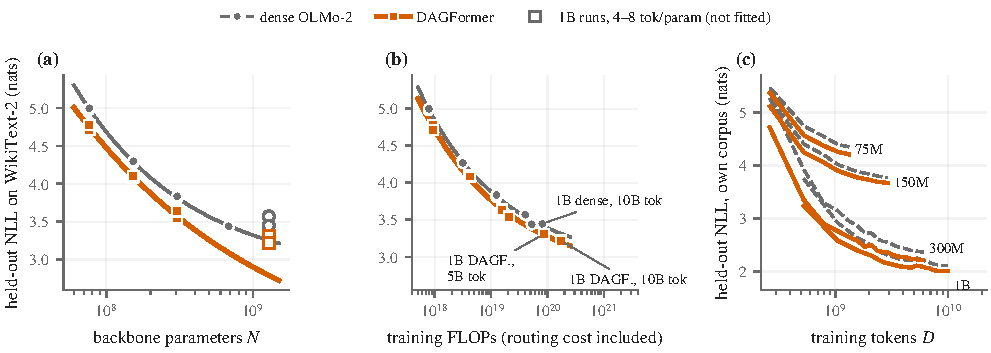
\includegraphics[width=\textwidth]{figures/fig_scaling.pdf}
\caption{Scaling of \dagf{} against matched dense OLMo-2. (a) Final WikiText-2 loss against backbone parameters for runs at 16 to 21 tokens per parameter, with power-law fits $L = E + A N^{-\alpha}$ per family (dense: 7 runs from 77M to 683M; \dagf{}: 6 runs from 77M to 304M, two corpora each); the 1B runs (hollow) are at 4 to 8 tokens per parameter and not fitted. (b) The same checkpoints and the 1B runs against training FLOPs with the routing cost included: the 1B \dagf{} at 5B tokens sits below the 1B dense model at 10B tokens at about the same compute. (c) Held-out loss along training for the four matched pairs, each on its own corpus's cache: the gap opens early in every run and persists.}
\label{fig:scaling}
\end{figure*}

At equal training compute the margin grows with size. For each \dagf{} run we read off the dense compute that reaches its loss on the fit $L=E+KC^{-\gamma}$ (Figure~\ref{fig:scaling}b) and divide by \dagf{}'s compute: this compute multiplier is 1.22 to 1.36 at 75M, 1.20 to 1.25 at 150M, 1.65 to 1.93 at 300M and 2.13 (5B tokens) to 2.39 (10B tokens) at 1B, although \dagf{}'s cost per token grows from 1.18$\times$ to 2.13$\times$. The cleanest comparison needs no fit: the 1B \dagf{} trained on 5B tokens ($8.6{\times}10^{19}$ FLOPs) beats the 1B dense model trained on 10B tokens ($8.1{\times}10^{19}$) on WikiText-2 (3.307 vs 3.446), MathInstruct (2.403 vs 2.483) and GSM8K (2.755 vs 2.900).

Extra parameters explain most of the gain at the smallest size and less than half at the next. Read through the dense curve of Figure~\ref{fig:scaling}a, a \dagf{} run is worth a dense model 1.20 to 1.27$\times$ its backbone size at 75M, 1.27 to 1.29$\times$ at 150M and 1.39 to 1.72$\times$ at 300M; counting the predictor's 29M to 32M parameters, the dense equivalent is 0.9 to 1.1$\times$ \dagf{}'s total size at 75M and 150M and 1.6$\times$ at 300M. The direct test agrees: the dense model with the routing parameters as extra width closes 70 to 89\% of the 75M gap and 4 to 42\% of the 150M gap across held-out sets, and \dagf{} stays ahead of it on every set at both sizes (Appendix~\ref{app:posthoc}).

\subsection{The predictor learns a static graph}
\label{sec:static}

What the predictor contributes is one graph per position, not per-token re-routing. Because it is a separate module, we can replace its per-token output by its mean over held-out windows (Table~\ref{tab:static_all}). At 300M and 1B the per-position mean costs at most 0.005 nats on WikiText-2 (3.544 vs 3.547; 3.219 vs 3.221 for the 1B at 10B tokens) and a single global mean 0.04 to 0.06, while the same replacement of the local correction channel costs 0.4 to 0.7 nats, more than the whole gap over dense. Swapping the predictor's output between windows (activation patching; \citealp{vig2020causal,meng2022rome,zhang2024patching}) changes the loss by at most 0.007 nats from 75M to 300M (the local channel: 0.56 to 1.29).

The token input is needed to learn the graph, not to apply it. In the predictor-only arm the per-token output carries 0.03 to 0.08 nats, yet replacing it by its position mean costs only 0.01 to 0.02, so the model routes per-token variation through a local channel when it has one. A table of the same weights trained from scratch with no input recovers only 17 to 23\% of the predictor-only arm's gain over dense (0.04 of 0.18 nats on the own cache, 0.06 of 0.39 on WikiText-2; Table~\ref{tab:locality}), and DenseFormer's learned static weights recover as little from 75M to 300M (at most 24\%; Table~\ref{tab:main}). The predictor is thus a parameterization that finds a good static graph, which Figure~\ref{fig:arch} shows for the 300M model and Appendix~\ref{app:topology} analyses.



\section{Structured pruning}
\label{sec:pruning}

\begin{table*}[t]
\centering\small
\setlength{\tabcolsep}{2pt}
% generated by paper/make_table_pruning.py from experiments/pruning/results/matched/summary.json -- do not edit
\begin{tabular*}{\textwidth}{@{\extracolsep{\fill}}l rrr rrr rrr}
\toprule
 & \multicolumn{3}{c}{75M} & \multicolumn{3}{c}{150M} & \multicolumn{3}{c}{300M} \\
\cmidrule(lr){2-4}\cmidrule(lr){5-7}\cmidrule(lr){8-10}
 & NLL $\downarrow$ & \multicolumn{2}{c}{increase (\%) $\downarrow$} & NLL $\downarrow$ & \multicolumn{2}{c}{increase (\%) $\downarrow$} & NLL $\downarrow$ & \multicolumn{2}{c}{increase (\%) $\downarrow$} \\
model & 0\% & 50\% & 70\% & 0\% & 50\% & 70\% & 0\% & 50\% & 70\% \\
\midrule
dense & 2.387 & 9.0 & \textbf{17.9} & 1.854 & 9.9 & 21.2 & 1.676 & 7.4 & 17.8 \\
DenseFormer & 2.383 & 9.5 & 18.7 & 1.830 & 9.5 & 20.7 & 1.641 & 7.9 & 18.5 \\
hyper-conn. & 2.306 & 9.5 & 19.5 & \pend{} & \pend{} & \pend{} & \pend{} & \pend{} & \pend{} \\
mHC & \pend{} & \pend{} & \pend{} & \pend{} & \pend{} & \pend{} & \pend{} & \pend{} & \pend{} \\
MUDDFormer & 2.362 & 10.6 & 22.3 & \textbf{1.692} & 12.8 & 28.6 & 1.558 & 9.3 & 22.0 \\
\dagf{} & \textbf{2.185} & \textbf{7.6} & 22.2 & 1.724 & \textbf{9.2} & \textbf{20.2} & \textbf{1.507} & \textbf{6.9} & \textbf{16.5} \\
\bottomrule
\end{tabular*}

\caption{Pruning during domain finetuning on MathInstruct, every model of Table~\ref{tab:main} from its own checkpoint (75M and 150M: 12B' corpus; 300M: 21B corpus): held-out NLL of the unpruned finetune (0\%) and the loss increase relative to it with 50\% and 70\% of attention heads and MLP channels removed by Taylor importance. Bold: best per column. \pend{}: running. All sparsities and the frozen-router controls are in Table~\ref{tab:pruning_full}.}
\label{tab:pruning}
\end{table*}

If the benefit is structural, a model whose heads read many earlier layers should lose less when units are removed, and the loss should not depend on the routers re-planning. We finetune each model on MathInstruct \citep{yue2023mammoth} for 2000 steps of 32K tokens; between steps 200 and 1400, attention heads and MLP channels are removed permanently on a cubic schedule \citep{zhu2017prune} by first-order Taylor importance on unit gates \citep{michel2019heads,molchanov2019taylor}, followed by 600 recovery steps. These are two of CoFi's unit types \citep{xia2022cofi}; every model of Table~\ref{tab:main} up to 300M is pruned from its own checkpoint with the same recipe, routers are never pruned, and we report backbone sparsity.

\dagf{} degrades more gracefully than dense in all but one setting (Table~\ref{tab:pruning}): relative to its own unpruned finetune it loses less with half the heads and channels removed at every size and with 70\% removed at 150M and 300M, while at 75M it loses 22.2 against 17.9\%, though its NLL stays 0.15 nats lower. Because it starts lower, with half its units removed it is better than the unpruned dense finetune at 75M and 300M and within 1.5\% of it at 150M.

The routed baselines degrade faster: at 300M, DenseFormer and MUDDFormer lose more than dense at both budgets, MUDDFormer most, and an earlier 150M comparison with MUDDFormer on a common corpus agrees (Table~\ref{tab:pruning_shared}).

The predictor does not re-plan. Freezing it during prune-finetune changes the 300M result by 0.003 nats at 50\%, as on the earlier pairs at 75M and 150M (Table~\ref{tab:pruning_shared}); freezing the local correction as well costs 0.025, so the local channel adapts a little, while freezing DenseFormer's depth weights or MUDDFormer's routers changes their results by at most 0.004 (Table~\ref{tab:pruning_full}). The advantage lies in the set of sources each head can draw on (Appendix~\ref{app:prunewhy} discusses why). It is not immunity: with units removed at random, both families lose much more and the gap shrinks at 75M (Appendix~\ref{app:prune}).

\section{Discussion}
\label{sec:discussion}

\paragraph{Is per-token routing necessary?} Dynamic cross-layer architectures motivate their routers by input dependence. Our separation shows that the gain of a token-reading predictor survives replacing its output by a per-position mean (Section~\ref{sec:static}), and that a model without hidden-state routers reaches nearly the same loss as one with them. The routing-source ablation (Table~\ref{tab:locality}, Appendix~\ref{app:locality}) varies only where $\valpha$ comes from in one 75M backbone: the shared predictor alone is within 0.017 nats of the full model and of the arm with local routers only. The benefit therefore lies mostly in the graph, a set of cross-layer connections and their weights, rather than in re-planning it per token. The graph is hard to learn without the input, though: static cross-layer weights trained directly recover little of the gain. Besides the input-free table of Section~\ref{sec:static}, DenseFormer is 0.01 to 0.03 nats worse than dense at 75M on every held-out set, closes 6 to 19\% of the gap at 150M and 16 to 24\% at 300M on every set but GSM8K, where it is 0.02 nats worse than dense, and static hyper-connections are up to 0.05 nats worse than dense at 75M and within 0.04 nats of it at 150M (Appendix~\ref{app:posthoc}). The separation does not show that a static graph is enough at inference for our shipped models: once a local channel is present the model comes to rely on its per-token output, and post-hoc sparsification of the learned graph costs a lot (Appendix~\ref{app:topology}). Distilling the learned graph into a fixed topology that a dense kernel can execute is a direction for future work.

\paragraph{One global predictor or routers distributed across layers?} At equal parameters a shared predictor matches per-layer routers at 75M (Table~\ref{tab:locality}), and sharing is what makes a token-reading predictor work: it beats independent per-layer predictors that see the same tokens but share nothing by 0.027 nats on the own cache and 0.049 on WikiText-2, with 7M fewer parameters, and the ordering holds on MathInstruct and GSM8K and after tuning (Appendix~\ref{app:locality}). Against MUDDFormer, whose per-layer routers read the hidden state, \dagf{} is ahead at two sizes and behind at one: MUDDFormer is 0.16 to 0.29 nats worse than \dagf{} at 75M and 0.05 to 0.10 nats worse at 300M on all five held-out sets, and 0.04 nats better at 150M on four of five, single seeds each. Loss alone does not separate the two designs at this scale. What separates them is what a separate module allows: the graph can be averaged, frozen and patched, which is how Section~\ref{sec:static} could locate the gain, and the pruned models degrade more gracefully. Whether a predictor can also beat per-layer routers on loss at larger scale, for instance by planning routing that no single layer can see, is untested.

\paragraph{Is the learned graph interpretable?} The predictor decides, before the backbone runs, which earlier results every head and layer combine, so its output is a natural place to audit or steer an inference pass: averaging, freezing and patching it are the causal interventions that generative interpretability asks of intermediate checkpoints \citep{yang2026generative}. We read the graph only in aggregate (Figure~\ref{fig:arch}, Appendix~\ref{app:topology}), and in the shipped models the per-token routing lives in the local channel, so we have not shown that the graph is meaningful to a human for a given input. A predictor-only \dagf{} at larger scale whose graph varies with the input in nameable ways, for instance by task or domain, could make the topology such a checkpoint, and routing among the outputs of specialised modules, which the modular variant begins to do (Appendix~\ref{app:modular}), points toward modular networks whose module outputs are themselves readable.

\section{Related work}
\label{sec:related}

\paragraph{Cross-layer connectivity.} After highway and residual skips \citep{srivastava2015highway,he2016resnet}, DenseNet \citep{huang2017densenet} connected every layer to every earlier one, and transparent attention \citep{bapna2018transparent}, ELMo \citep{peters2018elmo}, DenseFormer \citep{pagliardini2024denseformer} and LAuReL \citep{menghani2024laurel} learn static weights over layer outputs. Hyper-connections \citep{zhu2024hyperconnections} widen the residual stream into several streams with learnable, optionally input-dependent, depth and width connections; mHC \citep{mhc2026} constrains the residual-mixing matrices to be doubly stochastic so that their product across depth stays bounded; in the dynamic variants of both, a layer's coefficients depend on its incoming hidden state. MUDDFormer \citep{muddformer2025} generates per-position weights for the query, key, value and residual streams from each layer's hidden state. \dagf{} shares MUDDFormer's four-stream decomposition (per head for $q,k,v$) and differs in the source of the weights: one separate predictor over the tokens for all layers, with hidden-state routers as an optional correction.

\paragraph{Conditional computation.} Mixture-of-experts and mixture-of-depths models \citep{shazeer2017moe,fedus2022switch,raposo2024mod} route tokens to computation with a gate inside each routed layer. They choose which computation runs; \dagf{} chooses which earlier results a layer reads, for all layers at once.

\paragraph{Structured pruning.} Head and channel pruning with Taylor importance on a gradual schedule \citep{michel2019heads,molchanov2019taylor,zhu2017prune} covers two of CoFi's unit types \citep{xia2022cofi}; Sheared LLaMA \citep{xia2023sheared} prunes and then retrains. We use pruning as a probe of how a learned topology distributes information, not to propose a pruning method.

\section{Conclusion}

\dagf{} plans the cross-layer topology of a Transformer with one predictor that reads only the tokens. On matched pairs from 75M to 1B it improves loss at every size and at equal compute, its gain carries downstream, and it degrades more gracefully under structured pruning. Because the predictor is separate, the topology becomes an object that can be inspected and intervened on.

\section*{Limitations}
\label{sec:limitations}

\emph{Scale and seeds.} Our largest model has 1B parameters and is trained on 5 to 10B tokens, below its compute-optimal budget, and the fits pool runs from three tokenizations of Dolma. All pretraining runs but the 300M pair are single seeds; a second 300M seed moves each model by about 0.03 nats on WikiText-2 and MathInstruct and up to 0.08 on GSM8K, and the gap ranges from 0.26 to 0.31 nats over the four seed pairings, so differences below these are noise. The pruning cells are single runs. \emph{Cost.} Routing costs 1.18 to 2.13$\times$ dense FLOPs per token (measured 1.3 to 1.9$\times$ in inference and 1.3 to 2.2$\times$ in training); fused kernels would reduce this, and the predictor's 25.7M-parameter embedding could be tied to the backbone's. The shipped models rely on the local channel's per-token routing and cannot run with a fixed topology without retraining. \emph{Comparisons.} MUDDFormer trained with our recipe is 0.04 nats better than \dagf{} at 150M and 0.05 to 0.29 worse at 75M and 300M, each a single seed, so loss alone does not settle the comparison and the case for the separate predictor also rests on separability and pruning; the post-hoc baselines were trained at 1B for 5B tokens only and without hyper-connections, the parameter-matched dense models only at 75M and 150M, and only the 75M pair was swept over learning rates, where both models were still improving at the largest rate. \emph{Evaluation.} Models of this size sit near chance on harder benchmarks, and one LLM judge scored the chat comparison. \emph{Interpretability and scale.} We intervene on the learned graph only as a whole and inspect it only in aggregate. Whether its input-dependent part can be named, and whether the gains persist beyond 1B parameters, are left to follow-up work that scales \dagf{} up and analyses the predictor as the controller of the inference pass.

\bibliography{references}
% acl.sty already issues \bibliographystyle{acl_natbib}; a second one makes BibTeX complain.

\appendix

\section{Compute accounting}
\label{app:flops}
Forward MACs per token for the dense backbone are $\sum_{l=1}^{L}(4D^2 + 3DI) + VD$ plus attention over the context ($2TD$ per layer at sequence length $T$), with $D$ the model width, $I$ the MLP width and $V$ the vocabulary. \dagf{} adds, at every routed layer $l\ge2$, the projection of $l{-}1$ extra sources through the fused $q,k,v$ weights ($(l{-}1)\cdot 3D^2$), the per-head mixing sums ($l(3D + D)$), the predictor (embedding lookup, 2 encoder layers of width 256, trunk and per-layer heads) and the correction MLPs ($D\cdot 128 + 128\cdot(3H{+}1)\,l$ per layer). Training FLOPs are $6\times$ the forward MACs times tokens: the $C \approx 6N$ per token estimate of \citet{kaplan2020scaling} (a backward pass costs about twice the forward), applied to all the forward MACs above, so the unembedding, attention-context and routing terms that $6N$ leaves out are included. The ratios are 1.18 (75M), 1.33 (150M), 1.65 (300M) and 2.13 (1B); the predictor itself is under 2\% of the total, the source projections dominate. Table~\ref{tab:traincost} gives the measured training cost of every model of Table~\ref{tab:main}: forward and backward passes over 2 sequences of 1024 tokens with bf16 weights, as in pretraining, on one A100-40GB (median of 9 iterations after warm-up, no optimizer step). The baselines are measured at random initialization, since the weights do not change the speed. \dagf{} trains at 1.30 to 2.20$\times$ the dense time, close to its analytic ratio at 300M and 1B; mHC's reference operations, which run the Sinkhorn iterations unfused, are the slowest to train. Replacing the predictor by a constant table changes \dagf{}'s time by 1 to 3\%. At inference \dagf{} keeps every layer's output for the later layers to mix, so its peak memory for 8 sequences of 1024 tokens is 2.3 vs 1.9 GB (75M) to 7.8 vs 5.3 GB (1B). The 75M timings are dominated by per-kernel overhead (a dense forward pass takes 14 ms) and vary by up to 20\% between runs.

\begin{table*}[h]
\centering\footnotesize
% generated by paper/make_cost_tables.py from experiments/scaling/inference_cost.json (NVIDIA A100-SXM4-40GB) -- do not edit
\begin{tabular}{l r rrrrr r}
\toprule
 & \multicolumn{6}{c}{training: time per token relative to dense $\downarrow$} & inference \\
\cmidrule(lr){2-7}\cmidrule(lr){8-8}
size & dense (tok/s) & DenseFormer & hyper-conn. & mHC & MUDDFormer & \dagf{} & dense (tok/s) \\
\midrule
75M & 75.9K & 1.25 & 1.86 & 3.82 & 1.48 & 1.30 & 591K \\
150M & 57.3K & 1.23 & 1.96 & 3.59 & 1.61 & 1.40 & 313K \\
300M & 36.7K & 1.20 & 2.02 & 3.42 & 1.79 & 1.72 & 158K \\
1B & 14.7K & 1.18 & 2.03 & 2.42 & 1.65 & 2.20 & 52K \\
\bottomrule
\end{tabular}

\caption{Measured training cost: time per token of a forward and backward pass relative to the dense model of the same size (bf16 weights, 2 sequences of 1024 tokens, one A100-40GB, median of 9 iterations), with dense throughput in tokens per second for training and inference. Inference ratios are in Table~\ref{tab:main}.}
\label{tab:traincost}
\end{table*} The modular variant projects $2l{-}1$ sources per layer and costs 1.33 to 2.30$\times$.

\section{Held-out sets}
\label{app:cache}
The 21B-token tokenization's held-out tail is the last windows of its last shard, and the eight tokenization workers each took a contiguous block of Dolma's source-sorted file list, so that tail is templated instruction and Wikipedia text only; 21B-corpus runs score about 2.2 nats on it while scoring about 3.5 on WikiText-2. The tail is used only to compare runs within that corpus (the 300M three-way and the 1B pairs, where all models see the same training mix). The 1.7B-token slice used by the locality ablation has a similar single-source tail. All cross-corpus numbers in the paper are on WikiText-2, MathInstruct and GSM8K.

\section{Additional tables}
\label{app:tables}

\subsection{Downstream and chat per stage}
\label{app:downstream}
\begin{table*}[h]
\centering\scriptsize
\setlength{\tabcolsep}{1.5pt}
% generated by paper/make_table_downstream.py from experiments/results/lmeval/sft/SUMMARY_{300m,1b}.md -- do not edit
\begin{tabular*}{\textwidth}{@{\extracolsep{\fill}}lll rrrrrrrrrrrrr r}
\toprule
 & & & \multicolumn{14}{c}{accuracy (\%) $\uparrow$} \\
\cmidrule(lr){4-17}
size & stage & model & ARC-e & ARC-c & HSwag & PIQA & WinoG & OBQA & SciQ & BoolQ & LAMB & CSQA & SIQA & MathQA & GSM8K & \textbf{Mean} \\
\midrule
1B, 5B tok. & base & dense & 39.7 & 22.2 & 29.2 & 61.6 & \textbf{51.5} & 26.0 & 67.5 & \textbf{60.1} & 24.1 & 20.5 & 37.4 & 22.2 & \textbf{2.0} & 35.7 \\
 & & \dagf{} & \textbf{42.1} & \textbf{24.0} & \textbf{32.1} & \textbf{63.7} & 51.0 & \textbf{26.6} & \textbf{79.3} & 58.9 & \textbf{30.5} & \textbf{22.9} & \textbf{39.3} & \textbf{22.8} & \textbf{2.0} & \textbf{38.1} \\
\addlinespace[1pt]
 & +Alpaca & dense & 40.2 & \textbf{24.1} & 29.4 & 61.9 & \textbf{50.7} & 27.0 & 63.1 & \textbf{61.8} & 25.5 & 18.5 & 38.1 & 21.9 & \textbf{1.5} & 35.7 \\
 & & \dagf{} & \textbf{42.0} & \textbf{24.1} & \textbf{32.2} & \textbf{63.3} & 50.6 & \textbf{29.4} & \textbf{76.4} & 56.0 & \textbf{33.8} & \textbf{22.4} & \textbf{40.0} & \textbf{22.4} & \textbf{1.5} & \textbf{38.0} \\
\addlinespace[1pt]
 & +SmolTalk & dense & 38.2 & 22.5 & 29.3 & 62.1 & 50.4 & 26.6 & 60.4 & \textbf{62.1} & 18.8 & \textbf{20.8} & 37.8 & \textbf{23.7} & 1.0 & 34.9 \\
 & & \dagf{} & \textbf{41.1} & \textbf{22.8} & \textbf{32.0} & \textbf{63.4} & \textbf{50.6} & \textbf{27.8} & \textbf{75.2} & 61.1 & \textbf{27.1} & 20.6 & \textbf{38.0} & 23.0 & \textbf{1.5} & \textbf{37.2} \\
\bottomrule
\end{tabular*}

\caption{Table~\ref{tab:downstream} for the 1B models after 5B tokens. \dagf{} wins the chat comparison against the dense model after 5B tokens (0.58 and 0.59 after Alpaca and SmolTalk tuning) and against the dense model after 10B tokens (0.56 and 0.60).}
\label{tab:downstream_1b5b}
\end{table*}
Table~\ref{tab:downstream_full} gives every stage of Table~\ref{tab:downstream} and Table~\ref{tab:chat_full} every chat comparison, including the second instruction-tuning seed of the 300M pair. Repeating the 300M instruction tuning with a second seed moves the 12-task mean by at most 0.001 and the routed-minus-dense gaps by at most 0.003. Alpaca tuning leaves the multiple-choice mean within 0.002, SmolTalk lowers it by 0.7 to 1.4 points for every model, and GSM8K bits per byte improve by 0.13 to 0.25 after SmolTalk. Absolute judge scores are about 2 of 10 for every model; judging both orders cancels the judge's position bias (answer A wins 28 to 42\% of verdicts) at the cost of many ties.

\begin{table}[t]
\centering\footnotesize
\setlength{\tabcolsep}{2pt}
\begin{tabular}{llrrr}
\toprule
 & & MC acc. & \multicolumn{2}{c}{bits per byte $\downarrow$} \\
model & stage & $\uparrow$ & GSM8K & WikiText \\
\midrule
\multicolumn{5}{l}{\emph{300M, 21B corpus}} \\
dense & base & 0.369 & 1.458 & 1.128 \\
\dagf{} & base & \textbf{0.391} & \textbf{1.344} & \textbf{1.057} \\
dense & +Alpaca & 0.371 & 1.452 & 1.184 \\
\dagf{} & +Alpaca & \textbf{0.390} & \textbf{1.295} & \textbf{1.108} \\
dense & +SmolTalk & 0.364 & 1.269 & 1.309 \\
\dagf{} & +SmolTalk & \textbf{0.377} & \textbf{1.097} & \textbf{1.207} \\
\midrule
\multicolumn{5}{l}{\emph{1B, 21B corpus}} \\
dense 5B & base & 0.385 & 1.375 & 1.058 \\
dense 10B & base & 0.395 & 1.323 & 1.022 \\
\dagf{} 5B & base & 0.411 & 1.242 & 0.990 \\
\dagf{} 10B & base & \textbf{0.421} & \textbf{1.239} & \textbf{0.963} \\
dense 5B & +Alpaca & 0.385 & 1.348 & 1.090 \\
dense 10B & +Alpaca & 0.394 & 1.290 & 1.052 \\
\dagf{} 5B & +Alpaca & 0.410 & 1.200 & 1.021 \\
\dagf{} 10B & +Alpaca & \textbf{0.421} & \textbf{1.182} & \textbf{0.993} \\
dense 5B & +SmolTalk & 0.377 & 1.202 & 1.150 \\
dense 10B & +SmolTalk & 0.388 & 1.153 & 1.106 \\
\dagf{} 5B & +SmolTalk & 0.402 & 1.038 & 1.067 \\
\dagf{} 10B & +SmolTalk & \textbf{0.407} & \textbf{1.020} & \textbf{1.036} \\
\bottomrule
\end{tabular}
\caption{Downstream evaluation before (base) and after each instruction-tuning recipe, summarized (Table~\ref{tab:downstream} and Table~\ref{tab:downstream_1b5b} give per-task accuracy). MC acc.: mean accuracy over the twelve tasks (eleven multiple-choice and LAMBADA); GSM8K and WikiText: bits per byte on the gold GSM8K solutions and on WikiText (lower is better). One pretraining run per model. Repeating the 300M instruction tuning with a second seed moves the 12-task mean by at most 0.001 and WikiText bpb by less than 0.001 (BoolQ alone by up to 0.02), and the routed-minus-dense gaps reproduce within 0.003, so the tuning stage adds little noise; pretraining-seed variance is not measured. Shared-slice 75M and 150M pairs show the same pattern (Appendix~\ref{app:tables}).}
\label{tab:downstream_full}
\end{table}

\begin{table}[t]
\centering\footnotesize
\setlength{\tabcolsep}{2.2pt}
\begin{tabular}{llrc}
\toprule
SFT & \dagf{} vs.\ dense & win rate $\uparrow$ [CI] & W/L \\
\midrule
Alpaca & 300M vs.\ 300M, seed 1 & 0.57 [0.50, 0.64] & 16/10 \\
Alpaca & 300M vs.\ 300M, seed 2 & 0.61 [0.54, 0.67] & 19/8 \\
Alpaca & 1B@5B vs.\ 1B@5B & 0.58 [0.51, 0.66] & 26/12 \\
Alpaca & 1B@5B vs.\ 1B@10B & 0.56 [0.48, 0.64] & 23/17 \\
Alpaca & 1B@10B vs.\ 1B@10B & 0.56 [0.48, 0.63] & 19/14 \\
SmolTalk & 300M vs.\ 300M, seed 1 & \textbf{0.69} [0.63, 0.75] & 27/2 \\
SmolTalk & 300M vs.\ 300M, seed 2 & 0.64 [0.57, 0.71] & 30/5 \\
SmolTalk & 1B@5B vs.\ 1B@5B & 0.59 [0.52, 0.66] & 23/8 \\
SmolTalk & 1B@5B vs.\ 1B@10B & 0.60 [0.52, 0.67] & 27/10 \\
SmolTalk & 1B@10B vs.\ 1B@10B & 0.64 [0.57, 0.72] & 30/9 \\
\bottomrule
\end{tabular}
\caption{Judged chat quality on the 80 MT-Bench first turns. Win rate of \dagf{} with ties counted as half, averaged over both answer orders, with a 95\% bootstrap interval; W/L counts prompts where both orders agree. ``Seed 1/2'' are two independent instruction-tuning runs of both models from the same pretrained checkpoints. The judge prefers \dagf{} in every comparison; the interval excludes 0.5 in seven of ten.}
\label{tab:chat_full}
\end{table}

\subsection{Post-hoc baselines and learning rates}
\label{app:posthoc}

\begin{table*}[t]
\centering\footnotesize
\setlength{\tabcolsep}{3pt}
\begin{tabular}{llrrrr}
\toprule
run & size & WikiText-2 & MathInstruct & GSM8K & balanced \\
\midrule
dense & 75M & 4.997 & 4.271 & 4.242 & 5.167 \\
dense, hidden 656 & 75M & 4.769 & 4.057 & 4.052 & 4.961 \\
dense, 13 layers & 75M & 4.871 & 4.215 & 4.174 & 5.094 \\
DenseFormer & 75M & 5.027 & 4.303 & 4.249 & 5.196 \\
hyper-connections (static) & 75M & 5.042 & 4.301 & 4.246 & 5.191 \\
hyper-connections (DHC$\times$4) & 75M & 4.964 & 4.202 & 4.157 & 5.114 \\
MUDDFormer & 75M & 4.974 & 4.269 & 4.130 & 5.166 \\
\dagf{} & 75M & \textbf{4.711} & \textbf{3.984} & \textbf{3.973} & \textbf{4.937} \\
\midrule
dense & 150M & 4.268 & 3.599 & 3.608 & 4.471 \\
dense, hidden 864 & 150M & 4.199 & 3.537 & 3.599 & 4.409 \\
DenseFormer & 150M & 4.246 & 3.581 & 3.579 & 4.460 \\
hyper-connections (static) & 150M & 4.247 & 3.595 & 3.587 & 4.471 \\
MUDDFormer & 150M & \textbf{4.041} & \textbf{3.377} & \textbf{3.357} & \textbf{4.269} \\
\dagf{} & 150M & 4.085 & 3.383 & 3.402 & 4.305 \\
\midrule
dense & 300M & 3.808 & 2.742 & 3.232 & 3.832 \\
DenseFormer & 300M & 3.745 & 2.714 & 3.249 & 3.782 \\
MUDDFormer & 300M & 3.649 & 2.648 & 3.032 & 3.703 \\
\dagf{} & 300M & \textbf{3.544} & \textbf{2.565} & \textbf{2.937} & \textbf{3.606} \\
\bottomrule
\end{tabular}
\caption{Post-hoc baselines of Table~\ref{tab:main} on every common held-out set (NLL, nats per token). The parameter-matched dense models carry \dagf{}'s routing parameters as extra width (hidden 656 and 864; 107M and 182M parameters) or, at 75M, as extra depth (13 layers, 106M); hyper-connections are the static 4-stream variant. All runs of a size share recipe, data, tokens and seed; the 75M and 150M runs use the 12B' corpus and the 300M runs the 21B corpus.}
\label{tab:posthoc_sets}
\end{table*}

\begin{table}[t]
\centering\footnotesize
\setlength{\tabcolsep}{3pt}
\begin{tabular}{lrrrr}
\toprule
75M, WikiText-2 NLL $\downarrow$ & 2.5e-4 & 5e-4 & 1e-3 & 2e-3 \\
\midrule
dense & 5.878 & 4.997 & 4.654 & 4.563 \\
\dagf{} & 5.558 & 4.711 & 4.413 & 4.329 \\
gap & 0.32 & 0.29 & 0.24 & 0.23 \\
\bottomrule
\end{tabular}
\caption{Learning-rate sweep at 75M (12B' corpus, 1.58B tokens; the predictor's learning rate is 0.6$\times$ the backbone's). Both models improve up to the largest rate; the matched-rate gap moves from 0.32 to 0.23 nats and the best-against-best gap is 0.23. The same holds on MathInstruct, GSM8K and the balanced set (best-against-best narrows the 5e-4 gap by 5 to 19\%; 30\% on the Dolma tail).}
\label{tab:lrsweep}
\end{table}

\begin{table}[h]
\centering\scriptsize
\setlength{\tabcolsep}{2pt}
\begin{tabular}{lrrrr}
\toprule
routing source (75M) & routing & own & WikiText-2 & MC acc. \\
 & params & cache $\downarrow$ & NLL $\downarrow$ & w/o BoolQ $\uparrow$ \\
\midrule
none (dense) & 0 & 4.213 & 6.593 & 0.269 \\
static table, no token input & 500 & 4.171 & 6.529 & -- \\
per-layer predictors (unshared) & 35.6M & 4.058 & 6.256 & 0.271 \\
shared predictor only & 28.7M & 4.031 & 6.207 & 0.274 \\
local routers only & 29.1M & 4.018 & 6.176 & 0.275 \\
shared + local (\dagf{}) & 29.1M & \textbf{4.014} & \textbf{6.163} & \textbf{0.276} \\
\bottomrule
\end{tabular}
\caption{Routing-source ablation. Same 75M backbone, granularity and 1.57B tokens of a 1.7B-token Dolma slice; only the source of $\valpha$ changes. Static table: one weight per (layer, stream, head, source), no input; per-layer predictors: an encoder over the token ids per layer, nothing shared; local routers only: the correction MLPs with the predictor frozen at identity. Own cache: the run's held-out Dolma tail; MC: 11-task mean before tuning.}
\label{tab:locality}
\end{table}

\subsection{Training hyperparameters}
\label{app:hparams}
\begin{table*}[h]\centering\footnotesize\setlength{\tabcolsep}{3pt}
\begin{tabular}{lcccc}\toprule
size & 75M & 150M & 300M & 1B \\\midrule
layers / width / heads & 6 / 512 / 8 & 8 / 768 / 12 & 12 / 1024 / 16 & 16 / 2048 / 16 \\
MLP width & 2048 & 3072 & 4096 & 8192 \\
backbone params (M) & 76.6 & 152.6 & 304.1 & 1279.4 \\
routing params (M) & 29.1 & 30.0 & 32.3 & 36.7 \\
steps & 3000 & 6000 & 12000 & 9540 (+9540) \\
tokens (B) & 1.57 & 3.15 & 6.29 & 5.0 (10.0) \\
peak LR backbone / predictor & $5\mathrm{e}{-4}$ / $3\mathrm{e}{-4}$ & $5\mathrm{e}{-4}$ / $3\mathrm{e}{-4}$ & $5\mathrm{e}{-4}$ / $3\mathrm{e}{-4}$ & $4\mathrm{e}{-4}$ / $2\mathrm{e}{-4}$ \\
warmup steps & 300 & 300 & 300 & 500 \\
routed FLOPs / dense & 1.18 & 1.33 & 1.65 & 2.13 \\
\bottomrule\end{tabular}
\caption{Pretraining configurations. Common to all: 1024-token sequences, 512 sequences (524K tokens) per step, AdamW $(0.9, 0.95)$, weight decay 0.1, gradient clipping 1.0, linear decay to zero, bf16, tied embeddings, vocabulary 100,352 (the OLMo-2 tokenizer). Predictor: 256-d token and position embeddings, 2 causal encoder layers with 4 heads, trunk width 512, correction MLP width 128. The 1B runs were continued from 5B to 10B tokens with the schedule re-stretched and the learning rate re-warmed over 500 steps. Instruction tuning: global batch 64 sequences of 1024 tokens, cosine learning rate $2{\times}10^{-4}$ ($10^{-4}$ at 1B), assistant-only loss, ChatML format.}
\label{tab:hparams}\end{table*}

\subsection{Matched pairs on all held-out sets}
\label{app:pairs}
\begin{table*}[h]\centering\footnotesize\setlength{\tabcolsep}{2.5pt}
\begin{tabular}{llcccccccc}\toprule
size & corpus & \multicolumn{2}{c}{WikiText-2} & \multicolumn{2}{c}{MathInstruct} & \multicolumn{2}{c}{GSM8K} & \multicolumn{2}{c}{balanced Dolma} \\
 & & dense & \dagf{} & dense & \dagf{} & dense & \dagf{} & dense & \dagf{} \\\midrule
75M & 12B & 4.980 & 4.775 & 4.267 & 4.053 & 4.216 & 3.998 & 5.175 & 4.992 \\
75M & 12B' & 4.997 & 4.711 & 4.271 & 3.984 & 4.242 & 3.973 & 5.167 & 4.937 \\
150M & 12B & 4.297 & 4.100 & 3.630 & 3.424 & 3.626 & 3.465 & 4.514 & 4.334 \\
150M & 12B' & 4.268 & 4.085 & 3.599 & 3.383 & 3.608 & 3.402 & 4.471 & 4.305 \\
300M & 21B & 3.808 & 3.544 & 2.742 & 2.565 & 3.232 & 2.937 & 3.832 & 3.606 \\
300M, seed 2 & 21B & 3.835 & 3.530 & 2.774 & 2.562 & 3.308 & 2.897 & 3.855 & 3.608 \\
1B, 5B tok & 21B & 3.569 & 3.307 & 2.586 & 2.403 & 3.058 & 2.755 & 3.617 & 3.404 \\
1B, 10B tok & 21B & 3.446 & 3.219 & 2.483 & 2.321 & 2.900 & 2.644 & 3.501 & 3.314 \\
\bottomrule\end{tabular}
\caption{Held-out NLL (nats per token) of every matched pair on the four cross-corpus sets (final checkpoints): WikiText-2, MathInstruct, GSM8K and a source-balanced Dolma set (64 windows from each of 14 Dolma sources, drawn from files that no training corpus consumed; books, Wikipedia and open-web-math could not be represented). \dagf{} is lower in every cell; ``seed 2'' is the 300M pair repeated with a second pretraining seed.}
\label{tab:pairs_all}\end{table*}

\subsection{Gap along training}
\label{app:gapcurve}
The dense-minus-\dagf{} gap on each run's own held-out cache at matched steps (nats): 
75M (12B'): +0.096 @ 0.26B, +0.178 @ 0.53B, +0.175 @ 0.79B, +0.141 @ 1.32B; 150M (12B'): +0.160 @ 0.53B, +0.114 @ 1.32B, +0.107 @ 2.11B, +0.103 @ 2.91B; 300M (21B): +0.343 @ 1.31B, +0.207 @ 2.88B, +0.167 @ 4.46B, +0.161 @ 6.03B; 1B (21B): +0.197 @ 2.10B, +0.133 @ 4.72B, +0.116 @ 7.34B, +0.110 @ 9.96B. The gap opens within the first quarter of each run, peaks, and narrows slowly; the 1B entry is the 5B-token run.

\subsection{Router-locality ablation on all metrics}
\label{app:locality}
\begin{table*}[h]\centering\footnotesize\setlength{\tabcolsep}{2.5pt}
\begin{tabular}{lccccc}\toprule
routing source & own cache & WikiText-2 & MathInstruct & GSM8K & MC w/o BoolQ \\
 & & & & & base / Alpaca / SmolTalk \\\midrule
none (dense) & 4.213 & 6.593 & 5.373 & 5.404 & 0.269 / 0.278 / 0.293 \\
static learned table (no token input) & 4.176 & 6.529 & 5.243 & 5.279 & - \\
per-layer predictors (unshared) & 4.058 & 6.256 & 5.025 & 5.148 & 0.271 / 0.290 / 0.304 \\
shared predictor only & 4.031 & 6.207 & 4.981 & 5.116 & 0.274 / 0.289 / 0.301 \\
local routers only & 4.018 & 6.176 & 4.959 & 5.142 & 0.275 / 0.290 / 0.294 \\
shared + local (\dagf{}) & 4.014 & 6.163 & 4.932 & 5.080 & 0.276 / 0.290 / 0.302 \\
modular variant & 3.926 & 6.068 & 4.861 & 4.989 & 0.281 / 0.295 / 0.300 \\
modular + sparsity penalty & 4.091 & 6.274 & 5.139 & 5.229 & 0.273 / 0.286 / 0.300 \\
\bottomrule\end{tabular}
\caption{The 75M router-locality arms (1.57B tokens of a 1.7B-token Dolma slice, 4 GPUs each) on every held-out set, and the 11-task multiple-choice mean (without BoolQ, whose majority-class flips move the 12-task mean by up to 20 points at this size) before and after instruction tuning. The modular variant, which also routes the intra-layer edge, is best on loss at 75M; its routing cost is 1.33$\times$ dense here and it is not better than FourWay routing at 150M or 300M (Appendix~\ref{app:modular}).}
\label{tab:locality_all}\end{table*}

\subsection{Shared-slice 75M, 150M and 300M pairs downstream}
\label{app:shared_down}
\begin{table*}[h]\centering\footnotesize\setlength{\tabcolsep}{2.5pt}
\begin{tabular}{llcccc}\toprule
size & model & stage & MC acc. (12) & GSM8K bpb & WikiText bpb \\\midrule
75M & dense & base & 0.304 & 0.010 & 1.840 \\
75M & dense & +Alpaca & 0.309 & 0.010 & 1.801 \\
75M & dense & +SmolTalk & 0.309 & 0.015 & 1.613 \\
75M & \dagf{} & base & 0.316 & 0.025 & 1.759 \\
75M & \dagf{} & +Alpaca & 0.319 & 0.015 & 1.733 \\
75M & \dagf{} & +SmolTalk & 0.336 & 0.010 & 1.502 \\
150M & dense & base & 0.336 & 0.010 & 1.593 \\
150M & dense & +Alpaca & 0.337 & 0.015 & 1.560 \\
150M & dense & +SmolTalk & 0.340 & 0.020 & 1.337 \\
150M & \dagf{} & base & 0.361 & 0.005 & 1.519 \\
150M & \dagf{} & +Alpaca & 0.366 & 0.005 & 1.491 \\
150M & \dagf{} & +SmolTalk & 0.361 & 0.010 & 1.219 \\
300M & dense & base & 0.379 & 0.025 & 1.402 \\
300M & dense & +Alpaca & 0.367 & 0.025 & 1.403 \\
300M & dense & +SmolTalk & 0.368 & 0.015 & 1.145 \\
300M & \dagf{} & base & 0.397 & 0.015 & 1.331 \\
300M & \dagf{} & +Alpaca & 0.395 & 0.015 & 1.324 \\
300M & \dagf{} & +SmolTalk & 0.393 & 0.010 & 1.055 \\
\bottomrule\end{tabular}
\caption{The original 12B-slice pairs before and after instruction tuning (the 300M \dagf{} of this slice stopped at 9000 of 12000 steps, so its margin is a lower bound). Same metrics as Table~\ref{tab:downstream}.}
\label{tab:shared_down}\end{table*}

\subsection{Pruning: absolute losses, controls and immediate damage}
\label{app:prune}
\begin{table*}[h]\centering\footnotesize\setlength{\tabcolsep}{2.5pt}
\begin{tabular}{llcccc}\toprule
size & setting & dense & \dagf{} & peak post-prune dense & peak post-prune \dagf{} \\\midrule
75M & unpruned finetune & 2.388 & 2.223 & - & - \\
75M & 30\% heads+channels & 2.478 & 2.298 & 2.749 & 2.578 \\
75M & 50\% heads+channels & 2.590 & 2.391 & 2.841 & 2.604 \\
75M & 70\% heads+channels & 2.829 & 2.614 & 3.199 & 2.913 \\
75M & 50\%, random importance & 3.029 & 2.935 & 4.513 & 4.729 \\
75M & 33\% whole blocks & 2.610 & 2.547 & 4.760 & 4.377 \\
75M & 50\% whole blocks & 2.832 & 3.452 & 6.232 & 7.981 \\
150M & unpruned finetune & 1.883 & 1.743 & - & - \\
150M & 30\% heads+channels & 1.957 & 1.807 & 2.199 & 2.050 \\
150M & 50\% heads+channels & 2.071 & 1.899 & 2.286 & 2.068 \\
150M & 70\% heads+channels & 2.278 & 2.091 & 2.547 & 2.317 \\
150M & 50\%, random importance & 2.280 & 2.128 & 3.240 & 3.590 \\
150M & 33\% whole blocks & 2.200 & 2.170 & 3.945 & 3.726 \\
150M & 50\% whole blocks & 2.380 & 2.245 & 5.707 & 7.929 \\
300M & unpruned finetune & 1.608 & 1.488 & - & - \\
300M & 30\% heads+channels & 1.665 & 1.541 & 1.888 & 1.762 \\
300M & 50\% heads+channels & 1.762 & 1.620 & 1.904 & 1.772 \\
300M & 70\% heads+channels & 1.967 & 1.790 & 2.087 & 2.176 \\
\bottomrule\end{tabular}
\caption{Final held-out MathInstruct NLL after 2000 finetuning steps for every pruning run of the shared-slice pairs, and the highest NLL observed immediately after a pruning update (before recovery). Whole-block pruning removes entire attention or MLP blocks; the 75M \dagf{} at half the blocks is the one setting where it loses (Section~\ref{sec:pruning}). With random unit selection both families lose far more than with Taylor importance and the \dagf{} edge shrinks at 75M.}
\label{tab:prune_all}\end{table*}

\subsection{Static substitution on all held-out sets}
\label{app:static}
\begin{table*}[h]\centering\scriptsize\setlength{\tabcolsep}{3pt}
\begin{tabular}{llccccc}\toprule
model & set & intact & predictor $\to$ position mean & predictor $\to$ global mean & local $\to$ mean & both $\to$ mean \\\midrule
75M (locality arm, both) & wikitext2 & 6.164 & 6.161 & 6.162 & 6.582 & 6.595 \\
75M (locality arm, both) & mathinstruct & 4.933 & 4.928 & 4.934 & 5.267 & 5.272 \\
75M (locality arm, both) & gsm8k & 5.080 & 5.075 & 5.076 & 5.353 & 5.353 \\
75M (locality arm, both) & own & 4.009 & 4.012 & 4.038 & 4.465 & 4.502 \\
300M & wikitext2 & 3.544 & 3.547 & 3.604 & 4.251 & 4.297 \\
300M & mathinstruct & 2.565 & 2.556 & 2.600 & 3.065 & 3.065 \\
300M & gsm8k & 2.937 & 2.903 & 2.961 & 3.550 & 3.527 \\
300M & dolma21b & 2.222 & 2.223 & 2.261 & 2.920 & 2.962 \\
1B, 5B tok & wikitext2 & 3.307 & 3.310 & 3.364 & 3.996 & 4.027 \\
1B, 5B tok & mathinstruct & 2.403 & 2.405 & 2.446 & 2.940 & 2.959 \\
1B, 5B tok & gsm8k & 2.755 & 2.760 & 2.811 & 3.388 & 3.419 \\
1B, 5B tok & dolma21b & 2.076 & 2.077 & 2.117 & 2.782 & 2.812 \\
1B, 10B tok & wikitext2 & 3.219 & 3.221 & 3.281 & 3.916 & 3.950 \\
1B, 10B tok & mathinstruct & 2.321 & 2.322 & 2.366 & 2.849 & 2.868 \\
1B, 10B tok & gsm8k & 2.644 & 2.649 & 2.704 & 3.264 & 3.295 \\
1B, 10B tok & dolma21b & 2.005 & 2.005 & 2.049 & 2.758 & 2.791 \\
\bottomrule\end{tabular}
\caption{Held-out NLL when one routing channel is replaced by its mean over 128 held-out windows of the model's own corpus (`own' / `dolma21b' is that corpus's cache). The predictor's per-token output is replaceable at every size and on every set; the local correction channel's is not.}
\label{tab:static_all}\end{table*}

\subsection{Judged chat evaluation: categories and scores}
\label{app:chat}
\begin{table*}[h]\centering\footnotesize\setlength{\tabcolsep}{2.2pt}
\begin{tabular}{llcccccccc}\toprule
SFT & comparison & writing & roleplay & reasoning & math & coding & extraction & stem & humanities \\\midrule
Alpaca & 300M vs.\ 300M & 0.72 & 0.57 & 0.47 & 0.40 & 0.60 & 0.55 & 0.75 & 0.47 \\
Alpaca & 300M mod. vs.\ 300M & 0.80 & 0.53 & 0.42 & 0.50 & 0.50 & 0.72 & 0.55 & 0.68 \\
Alpaca & 1B@5B vs.\ 1B@5B & 0.55 & 0.60 & 0.42 & 0.45 & 0.42 & 0.62 & 0.75 & 0.85 \\
Alpaca & 1B@5B vs.\ 1B@10B & 0.42 & 0.82 & 0.50 & 0.28 & 0.53 & 0.65 & 0.53 & 0.75 \\
Alpaca & 1B@10B vs.\ 1B@10B & 0.40 & 0.75 & 0.42 & 0.33 & 0.65 & 0.65 & 0.53 & 0.75 \\
SmolTalk & 300M vs.\ 300M & 0.82 & 0.82 & 0.53 & 0.80 & 0.65 & 0.57 & 0.60 & 0.72 \\
SmolTalk & 300M mod. vs.\ 300M & 0.68 & 0.62 & 0.35 & 0.50 & 0.55 & 0.57 & 0.70 & 0.62 \\
SmolTalk & 1B@5B vs.\ 1B@5B & 0.78 & 0.62 & 0.55 & 0.53 & 0.42 & 0.57 & 0.70 & 0.53 \\
SmolTalk & 1B@5B vs.\ 1B@10B & 0.82 & 0.62 & 0.50 & 0.38 & 0.60 & 0.68 & 0.65 & 0.53 \\
SmolTalk & 1B@10B vs.\ 1B@10B & 0.80 & 0.60 & 0.78 & 0.55 & 0.50 & 0.65 & 0.57 & 0.70 \\
Alpaca & 300M s2 vs.\ 300M s2 & 0.55 & 0.47 & 0.68 & 0.60 & 0.60 & 0.60 & 0.72 & 0.62 \\
Alpaca & 300M mod. s2 vs.\ 300M s2 & 0.90 & 0.57 & 0.57 & 0.53 & 0.42 & 0.65 & 0.70 & 0.47 \\
SmolTalk & 300M s2 vs.\ 300M s2 & 0.78 & 0.68 & 0.50 & 0.68 & 0.65 & 0.47 & 0.50 & 0.88 \\
SmolTalk & 300M mod. s2 vs.\ 300M s2 & 0.53 & 0.60 & 0.50 & 0.78 & 0.62 & 0.57 & 0.50 & 0.50 \\
\bottomrule\end{tabular}
\caption{Per-category win rate of \dagf{} (10 prompts per category, so $\pm 0.15$ is noise). ``300M mod.'' is the modular variant.}
\label{tab:chat_cats}\end{table*}
\begin{table*}[h]\centering\footnotesize\setlength{\tabcolsep}{3pt}
\begin{tabular}{lccc}\toprule
model & mean score (1--10) & answer tokens & ended on end-of-turn \\\midrule
300M dense / Alpaca & 1.91 & 109 & 0.74 \\
300M \dagf{} / Alpaca & 2.15 & 109 & 0.72 \\
300M modular / Alpaca & 1.95 & 114 & 0.71 \\
1B dense 5B / Alpaca & 2.06 & 103 & 0.74 \\
1B \dagf{} 5B / Alpaca & 2.14 & 122 & 0.75 \\
1B dense 10B / Alpaca & 2.19 & 111 & 0.71 \\
1B \dagf{} 10B / Alpaca & 2.33 & 122 & 0.70 \\
300M dense / SmolTalk & 2.12 & 210 & 0.34 \\
300M \dagf{} / SmolTalk & 2.52 & 210 & 0.35 \\
300M modular / SmolTalk & 2.34 & 208 & 0.38 \\
1B dense 5B / SmolTalk & 2.06 & 210 & 0.34 \\
1B \dagf{} 5B / SmolTalk & 2.35 & 200 & 0.40 \\
1B dense 10B / SmolTalk & 2.12 & 204 & 0.38 \\
1B \dagf{} 10B / SmolTalk & 2.52 & 210 & 0.38 \\
300M dense seed 2 / Alpaca & 1.99 & 117 & 0.66 \\
300M \dagf{} seed 2 / Alpaca & 2.14 & 112 & 0.71 \\
300M modular seed 2 / Alpaca & 2.01 & 107 & 0.74 \\
300M dense seed 2 / SmolTalk & 2.16 & 211 & 0.31 \\
300M \dagf{} seed 2 / SmolTalk & 2.45 & 199 & 0.41 \\
300M modular seed 2 / SmolTalk & 2.40 & 206 & 0.38 \\
\bottomrule\end{tabular}
\caption{Single-answer judge scores (MT-Bench single-answer prompt, same judge), mean answer length and the fraction of answers that stopped on the end-of-turn token rather than the 256-token cap. Scores sit near 2 of 10 for every model at this scale; the pairwise win rate is the informative number.}
\label{tab:chat_scores}\end{table*}


\section{Topology analysis}
\label{app:topology}
Over 128 held-out windows of each model's own corpus we record the predictor's and the correction channel's outputs. Averaged over tokens, most mixing mass sits on skip sources rather than the previous layer: the previous layer carries 17 to 61\% of the $|\alpha|$ mass for queries, 12 to 45\% for keys, only 2 to 24\% for values and 4 to 68\% for the residual (300M and 1B), and 2 to 5 sources per head exceed 5\% of the head's largest weight. Per-token spread relative to the mean is 0.05 to 0.19 for the predictor and 0.5 to 1.4 for the corrections. The graph is used densely: zeroing at inference the quarter of hyperconnection entries with the smallest mean $|\alpha|$ (both channels, per-token routing otherwise intact) costs 0.27 nats at 300M and 0.15 to 0.22 at 1B on WikiText-2, half of them costs about 1.8 nats, and removing every skip so that each layer reads only its predecessor raises the loss to 9 to 10 nats; sparsifying the topology for inference would need retraining rather than post-hoc masking.

\section{Pruning: all runs}
\label{app:prunefull}
Table~\ref{tab:pruning_full} lists every matched-corpus pruning run behind Table~\ref{tab:pruning}, and Table~\ref{tab:pruning_shared} the earlier study on the original 12B-slice pairs, which Figure~\ref{fig:pruning} plots.

\begin{table*}[h]
\centering\small
\setlength{\tabcolsep}{2pt}
% generated by paper/make_table_pruning.py from experiments/pruning/results/matched/summary.json -- do not edit
\begin{tabular*}{\textwidth}{@{\extracolsep{\fill}}ll rrrr rr}
\toprule
 & & \multicolumn{4}{c}{held-out NLL $\downarrow$ at sparsity} & \multicolumn{2}{c}{NLL at 50\%, routers frozen} \\
\cmidrule(lr){3-6}\cmidrule(lr){7-8}
size & model & 0\% & 30\% & 50\% & 70\% & all routers & predictor only \\
\midrule
75M & dense & 2.387 & 2.475 & 2.602 & 2.815 & -- & -- \\
 & DenseFormer & 2.383 & 2.482 & 2.610 & 2.829 & 2.640 & -- \\
 & hyper-conn. & 2.306 & 2.400 & 2.526 & 2.756 & 2.517 & -- \\
 & mHC & \pend{} & \pend{} & \pend{} & \pend{} & \pend{} & -- \\
 & MUDDFormer & 2.362 & 2.461 & 2.612 & 2.889 & 2.618 & -- \\
 & \dagf{} & \textbf{2.185} & \textbf{2.258} & \textbf{2.350} & \textbf{2.669} & 2.371 & 2.365 \\
\addlinespace[2pt]
150M & dense & 1.854 & 1.930 & 2.038 & 2.248 & -- & -- \\
 & DenseFormer & 1.830 & 1.901 & 2.004 & 2.210 & 2.004 & -- \\
 & hyper-conn. & \pend{} & \pend{} & \pend{} & \pend{} & \pend{} & -- \\
 & mHC & \pend{} & \pend{} & \pend{} & \pend{} & \pend{} & -- \\
 & MUDDFormer & \textbf{1.692} & 1.790 & 1.908 & 2.176 & 1.905 & -- \\
 & \dagf{} & 1.724 & \textbf{1.788} & \textbf{1.882} & \textbf{2.073} & 1.894 & 1.883 \\
\addlinespace[2pt]
300M & dense & 1.676 & 1.722 & 1.799 & 1.975 & -- & -- \\
 & DenseFormer & 1.641 & 1.690 & 1.771 & 1.945 & 1.770 & -- \\
 & hyper-conn. & \pend{} & \pend{} & \pend{} & \pend{} & \pend{} & -- \\
 & mHC & \pend{} & \pend{} & \pend{} & \pend{} & \pend{} & -- \\
 & MUDDFormer & 1.558 & 1.611 & 1.702 & 1.901 & 1.706 & -- \\
 & \dagf{} & \textbf{1.507} & \textbf{1.549} & \textbf{1.610} & \textbf{1.756} & 1.635 & 1.613 \\
\bottomrule
\end{tabular*}

\caption{All matched-corpus pruning runs of Table~\ref{tab:pruning}: held-out MathInstruct NLL after 2000 steps at 0 to 70\% sparsity, and at 50\% with every router frozen during finetuning (DenseFormer's depth weights, the hyper-connection modules, MUDDFormer's routers, \dagf{}'s predictor and local correction) or, for \dagf{}, only the predictor. Bold: best per size and column. \pend{}: running.}
\label{tab:pruning_full}
\end{table*}

\begin{table*}[h]
\centering\small
\setlength{\tabcolsep}{2pt}
% generated by paper/make_table_pruning.py from experiments/pruning/results/prune_summary.md and experiments/coherence/results/exp3/prune_summary.md -- do not edit
\begin{tabular*}{\textwidth}{@{\extracolsep{\fill}}ll rrrr rr r}
\toprule
 & & \multicolumn{4}{c}{held-out NLL $\downarrow$} & \multicolumn{2}{c}{increase (\%)} & frozen \\
\cmidrule(lr){3-6}\cmidrule(lr){7-8}\cmidrule(lr){9-9}
size & model & 0\% & 30\% & 50\% & 70\% & at 50\% & at 70\% & NLL at 50\% \\
\midrule
75M & dense & 2.388 & 2.478 & 2.590 & 2.829 & 8.4 & 18.5 & -- \\
 & \dagf{} & \textbf{2.223} & \textbf{2.298} & \textbf{2.391} & \textbf{2.614} & 7.5 & 17.6 & 2.388 \\
\addlinespace[2pt]
150M & dense & 1.883 & 1.957 & 2.071 & 2.278 & 10.0 & 21.0 & -- \\
 & \dagf{} & \textbf{1.743} & \textbf{1.807} & \textbf{1.899} & \textbf{2.091} & 8.9 & 20.0 & 1.899 \\
\addlinespace[2pt]
300M & dense & 1.608 & 1.665 & 1.762 & 1.967 & 9.6 & 22.3 & -- \\
 & \dagf{} & \textbf{1.488} & \textbf{1.541} & \textbf{1.620} & \textbf{1.790} & 8.9 & 20.3 & -- \\
\addlinespace[2pt]
150M$^\ast$ & dense & 2.075 & 2.157 & 2.273 & 2.507 & 9.5 & 20.8 & -- \\
 & MUDDFormer & 1.935 & 2.037 & 2.153 & 2.366 & 11.3 & 22.3 & 2.150 \\
 & \dagf{} & \textbf{1.924} & \textbf{1.990} & \textbf{2.087} & \textbf{2.268} & 8.5 & 17.9 & 2.078 \\
\bottomrule
\end{tabular*}

\caption{The earlier pruning study on the original 12B-slice pairs (75M to 300M) and a 150M comparison with MUDDFormer on a common corpus (150M$^\ast$): held-out NLL, the loss increase relative to the same model's unpruned finetune, and the NLL at 50\% with the predictor (\dagf{}) or every router (MUDDFormer) frozen. Bold: best per block and column.}
\label{tab:pruning_shared}
\end{table*}

\section{Why reading many layers may soften pruning}
\label{app:prunewhy}
\begin{figure*}[h]
\centering
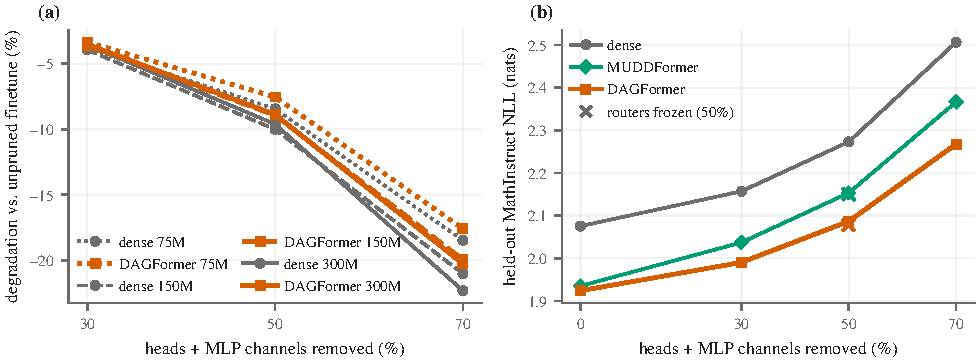
\includegraphics[width=0.82\textwidth]{figures/fig_pruning.pdf}
\caption{Pruning during domain finetuning on MathInstruct. (a) Held-out NLL relative to the same model's unpruned finetune with 30/50/70\% of heads and MLP channels removed, the original 12B-slice pairs at three sizes: \dagf{} loses less at every budget, more so at higher sparsity. (b) 150M, common corpus: \dagf{} against MUDDFormer and dense, equal unpruned; \dagf{} ahead by 0.05/0.07/0.10 nats at 30/50/70\%; frozen routers (crosses) change neither.}
\label{fig:pruning}
\end{figure*}
Figure~\ref{fig:pruning} plots the results of Table~\ref{tab:pruning_shared}. A head that reads several earlier layers has several routes to the information it needs, so removing one unit removes one route rather than the only one. The frozen-router result is consistent with this reading: the gain needs no re-routing, only the connections that training put in place. The random-pruning control shows its limit, since the advantage shrinks when the removed units are not the least important ones. We have not tested the redundancy hypothesis directly, for instance by counting alternative paths around removed heads.

\section{The modular variant}
\label{app:modular}
\begin{figure*}[t]
\centering
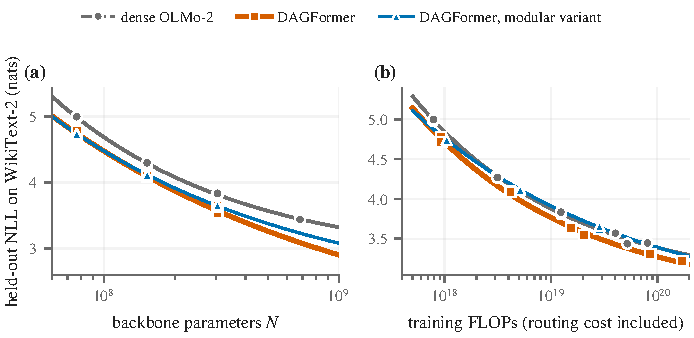
\includegraphics[width=0.72\textwidth]{figures/fig_scaling_modular.pdf}
\caption{The modular variant against \dagf{} (FourWay routing) and dense OLMo-2, as in Figure~\ref{fig:scaling}a and~b: (a) final WikiText-2 loss against backbone parameters, (b) against training FLOPs with the routing cost included. On the same corpus, modular routing is 0.03 nats behind FourWay at 75M and 150M and 0.08 behind at 300M, and per FLOP it does not repay its extra cost above 75M.}
\label{fig:modular}
\end{figure*}
Figure~\ref{fig:modular} places the modular variant in the scaling plots of Figure~\ref{fig:scaling}. In FourWay routing the sources are layer outputs, so the attention-to-MLP edge inside a layer, the block-to-everything-downstream edges and the final read-out are fixed. A \emph{modular} variant makes the sources the module outputs (embedding, then each layer's attention and MLP outputs) and adds a routed MLP input and a routed final read-out, so every intermodular edge is predicted; its routing is $2l{-}1$ sources per layer and costs 1.33$\times$ (75M) to 2.30$\times$ (300M) dense FLOPs. At 300M on the 21B corpus, FourWay beats modular on every held-out set (WikiText-2 3.544 vs 3.628, Dolma tail 2.221 vs 2.268, MathInstruct 2.565 vs 2.616, GSM8K 2.937 vs 3.093), and the modular compute multiplier is 1.15 at 75M and 0.81 to 0.93 at 150M to 300M (its extra FLOPs are not repaid). Modular routing is better in one setting: whole-block pruning scored by the mass of a module's routing column, where it beats FourWay's Taylor-pruned blocks at 150M (2.015 vs 2.044 nats at a third of the blocks removed, 2.130 vs 2.229 at half). We therefore ship FourWay and leave modular routing as an ablation.

\end{document}
